% -*- Mode:TeX -*-

%% IMPORTANT: The official thesis specifications are available at:
%%            http://libraries.mit.edu/archives/thesis-specs/
%%
%%            Please verify your thesis' formatting and copyright
%%            assignment before submission.  If you notice any
%%            discrepancies between these templates and the 
%%            MIT Libraries' specs, please let us know
%%            by e-mailing thesis@mit.edu

%% The documentclass options along with the pagestyle can be used to generate
%% a technical report, a draft copy, or a regular thesis.  You may need to
%% re-specify the pagestyle after you \include  cover.tex.  For more
%% information, see the first few lines of mitthesis.cls. 

%\documentclass[12pt,vi,twoside]{mitthesis}
%%
%%  If you want your thesis copyright to you instead of MIT, use the
%%  ``vi'' option, as above.
%%
%\documentclass[12pt,twoside,leftblank]{mitthesis}
%%
%% If you want blank pages before new chapters to be labelled ``This
%% Page Intentionally Left Blank'', use the ``leftblank'' option, as
%% above. 

\documentclass[12pt,a4,twoside,vi,singlespace,draft,drafthead]{mitthesis}
\pagestyle{plain}

%% This bit allows you to either specify only the files which you wish to
%% process, or `all' to process all files which you \include.
%% Krishna Sethuraman (1990).

%\typein [\files]{Enter file names to process, (chap1,chap2 ...), or `all' to
%process all files:}
%\def\all{all}
%\ifx\files\all \typeout{Including all files.} \else \typeout{Including only \files.} \includeonly{\files} \fi

\begin{document}

% -*-latex-*-
% 
% For questions, comments, concerns or complaints:
% thesis@mit.edu
% 
%
% $Log: cover.tex,v $
% Revision 1.8  2008/05/13 15:02:15  jdreed
% Degree month is June, not May.  Added note about prevdegrees.
% Arthur Smith's title updated
%
% Revision 1.7  2001/02/08 18:53:16  boojum
% changed some \newpages to \cleardoublepages
%
% Revision 1.6  1999/10/21 14:49:31  boojum
% changed comment referring to documentstyle
%
% Revision 1.5  1999/10/21 14:39:04  boojum
% *** empty log message ***
%
% Revision 1.4  1997/04/18  17:54:10  othomas
% added page numbers on abstract and cover, and made 1 abstract
% page the default rather than 2.  (anne hunter tells me this
% is the new institute standard.)
%
% Revision 1.4  1997/04/18  17:54:10  othomas
% added page numbers on abstract and cover, and made 1 abstract
% page the default rather than 2.  (anne hunter tells me this
% is the new institute standard.)
%
% Revision 1.3  93/05/17  17:06:29  starflt
% Added acknowledgements section (suggested by tompalka)
% 
% Revision 1.2  92/04/22  13:13:13  epeisach
% Fixes for 1991 course 6 requirements
% Phrase "and to grant others the right to do so" has been added to 
% permission clause
% Second copy of abstract is not counted as separate pages so numbering works
% out
% 
% Revision 1.1  92/04/22  13:08:20  epeisach

% NOTE:
% These templates make an effort to conform to the MIT Thesis specifications,
% however the specifications can change.  We recommend that you verify the
% layout of your title page with your thesis advisor and/or the MIT 
% Libraries before printing your final copy.
\title{Architecture of a Quantum Computer}

\author{Sebastian Pauka}
% If you wish to list your previous degrees on the cover page, use the 
% previous degrees command:
%       \prevdegrees{A.A., Harvard University (1985)}
% You can use the \\ command to list multiple previous degrees
%       \prevdegrees{B.S., University of California (1978) \\
%                    S.M., Massachusetts Institute of Technology (1981)}
\department{The School of Physics}

% If the thesis is for two degrees simultaneously, list them both
% separated by \and like this:
% \degree{Doctor of Philosophy \and Master of Science}
\degree{Doctor of Philosophy}

% As of the 2007-08 academic year, valid degree months are September, 
% February, or June.  The default is June.
\degreemonth{June}
\degreeyear{2019}
\thesisdate{June 30, 2019}

%% By default, the thesis will be copyrighted to MIT.  If you need to copyright
%% the thesis to yourself, just specify the `vi' documentclass option.  If for
%% some reason you want to exactly specify the copyright notice text, you can
%% use the \copyrightnoticetext command.  
%\copyrightnoticetext{\copyright IBM, 1990.  Do not open till Xmas.}

% If there is more than one supervisor, use the \supervisor command
% once for each.
\supervisor{David Reilly}{Professor}

% This is the department committee chairman, not the thesis committee
% chairman.  You should replace this with your Department's Committee
% Chairman.
% \chairman{Arthur C. Smith}{Chairman, Department Committee on Graduate Theses}

% Make the titlepage based on the above information.  If you need
% something special and can't use the standard form, you can specify
% the exact text of the titlepage yourself.  Put it in a titlepage
% environment and leave blank lines where you want vertical space.
% The spaces will be adjusted to fill the entire page.  The dotted
% lines for the signatures are made with the \signature command.
\maketitle

% The abstractpage environment sets up everything on the page except
% the text itself.  The title and other header material are put at the
% top of the page, and the supervisors are listed at the bottom.  A
% new page is begun both before and after.  Of course, an abstract may
% be more than one page itself.  If you need more control over the
% format of the page, you can use the abstract environment, which puts
% the word "Abstract" at the beginning and single spaces its text.

%% You can either \input (*not* \include) your abstract file, or you can put
%% the text of the abstract directly between the \begin{abstractpage} and
%% \end{abstractpage} commands.

% First copy: start a new page, and save the page number.
\cleardoublepage
% Uncomment the next line if you do NOT want a page number on your
% abstract and acknowledgments pages.
% \pagestyle{empty}
\begin{abstractpage}
% $Log: abstract.tex,v $
% Revision 1.1  93/05/14  14:56:25  starflt
% Initial revision
% 
% Revision 1.1  90/05/04  10:41:01  lwvanels
% Initial revision
% 
%
%% The text of your abstract and nothing else (other than comments) goes here.
%% It will be single-spaced and the rest of the text that is supposed to go on
%% the abstract page will be generated by the abstractpage environment.  This
%% file should be \input (not \include 'd) from cover.tex.
!!Abstract Goes Here!!
\end{abstractpage}

% Additional copy: start a new page, and reset the page number.  This way,
% the second copy of the abstract is not counted as separate pages.
% Uncomment the next 6 lines if you need two copies of the abstract
% page.
% \setcounter{page}{\thesavepage}
% \begin{abstractpage}
% % $Log: abstract.tex,v $
% Revision 1.1  93/05/14  14:56:25  starflt
% Initial revision
% 
% Revision 1.1  90/05/04  10:41:01  lwvanels
% Initial revision
% 
%
%% The text of your abstract and nothing else (other than comments) goes here.
%% It will be single-spaced and the rest of the text that is supposed to go on
%% the abstract page will be generated by the abstractpage environment.  This
%% file should be \input (not \include 'd) from cover.tex.
!!Abstract Goes Here!!
% \end{abstractpage}

\cleardoublepage

\bgroup
\let\addcontentsline=\nocontentsline
\section*{Acknowledgments}
\egroup
\addtocontents{toc}{\protect\setcounter{tocdepth}{-1}}
\addcontentsline{toc}{chapter}{Acknowledgements}
\addtocontents{toc}{\protect\setcounter{tocdepth}{2}}

It was more than six years ago now that I found myself choosing between a research career in physics and
one in computer science. At the time, it was a difficult choice, but with the benefit of hindsight, I have
no doubts that I made the right call. That is to a considerable degree due to amazing people I've had the
opportunity to work with.

First, I would like to thank my supervisor David Reilly. Without his gently cajoling at the beginning, I may have ended
up somewhere entirely different. Since then, I've learned an enormous amount through his teaching and through
constant and entertaining discussions. Without his support and guidance, I can't imagine having had the
fantastic Ph.D. I have had. More than that, under his supervision, I've met extraordinary people, traveled
to countless conferences and seen the lab grow from a single fridge and a smattering of students, to an empire
with seven fridges (a number which I think is becoming eight as I write this) and an innumerable number
of people. I still remember our road trip down California and all the discussions it provoked as one of the best times I've had.
I am also grateful to Andrew Doherty who gave his time and counsel, both in physics (of which his
knowledge seems endless) and in life, despite his enormously busy schedule. Under his tutelage, I learned so much about
physics and the community, understanding to which I still regularly refer. To Maja Cassidy, who joined only recently
but has had such a massive impact on the science that I (and indeed the whole lab) has been able to do, thank you
for your support and direction, I gained so much insight in our conversations over the past year.

To the entire Quantum Nanoscience Lab, I want to express my heartfelt gratitude. The people who I've had a chance
to work with have all enriched my life, professional and personal, enormously. I can't think of a better group of
people to have worked with over the years.

To John Hornibrook, I think it was only a few months ago that I learned that our pairing in the early days of Honours
was a last minute arrangement. Thank you for patiently explaining the fundamentals of physics to a hopelessly lost
student. Without your encouragement in the early days, I can't imagine how I would have made it this far. The lab
has been a pleasure to work in by your side, and I hope we can continue to swap programming oddities well into the future.

To James Colless, who is both an unending fountain of knowledge and who taught me how to survive in a physics lab,
thank you for giving me such a great intuitive understanding of the work we do. I enjoyed working and learning with
you immensely, and to top it off, our time traveling was the best!

Xanthe Croot is just about the most joyous, tireless, optimistic and loud person I know, who brings so much to any
workplace, all the while being one of the best physicists I know. Thank you for the constant arguments(/discussions).
Even though I think we freaked out anyone walking past, they were amongst the most informative times I had.
Thanks also for pushing me to do more outside of the lab, whether it was running a half marathon or singing Mariah Carey
loudly in the lab, I grew a great deal as a result.

Last amongst the original quantum dot crew, to Alice Mahoney, thank you for being at first a fantastic mentor and then
a great friend. I still remember you stressing about my honors talk and thesis far more than me, which, you know, fair,
and as a result pushing me to do better and be better. You made the lab, and everyone in it better organized, more diligently
logbooked and pushed me to be meticulous with the science. The brunches were fun too.

To Ewa Rej, thanks for being a fantastic labmate and friend. Our trivia Wednesdays are a social event I've never quite managed
to repeat, and our conversations have meant so much over the years. MC Jarratt, thanks for being an excellent lab buddy, drinking
partner, and friend. Our road trips through America were, without a doubt, a highlight of my Ph.D., and I can't wait to go on another
craft brewery crawl. To Steven Waddy, your endless knowledge about the minutiae of physics and electronics has taught me so much and made the lab a surprisingly insightful place to work. To Ian Conway-Lamb, your help with PCB, FPGA, and mechanical engineering
was invaluable over the years, our movie nights never quite recovered after you left. To my coffee friend over in NMR: Tom Boele,
thanks for the discussions and support particularly in the last few weeks of the Ph.D. The chance to escape writing has been
indispensable for my sanity. To Torsten Gaebel, thanks for all your help fixing things, for keeping us all safe and for the
company on our many nights to the pub.

To everyone else in the QNL, thank you. The ASIC team of Kushal Das, Ali Moini and YuanYuan Yang, learning about transistors,
CMOS design, and working with you on Mulberry and Gooseberry has been invaluable. The FPGA and RF team of Jon Knoblauch, Deshan Govender
and Neil Dick, thanks for the insights about FPGA design, RF engineering, and whiskey. And remaining engineers and scientists,
Jana Darulova, Brendan Altus, Tim Newman, and Andrew Kelly, thanks for all the conversations over the years. I can't imagine a workplace
this good, and it's all down to the fantastic people in this lab.

To all the others who have supported me scientifically thank you. To the entire team at ANFF UNSW, Joanna Syzmanska, Nadia Court,
and Pierrette Michaux, thank you for your help with fabrication and for training me in the early days. To all the growers, Hong Lu and Art Gossard
from UCSB, and Geoff Gardner, John Watson and Mike Manfra from Purdue University, who have supplied us with high-quality material without
which we would not have been able to do any science, thank you. To the entire team at Copenhagen who kindly hosted me over a period of
3 months, it was an amazingly productive time, and everyone there made me feel like I had a true second home. In particular, I would like to
thank Charlie Marcus for welcoming me as if I was a longtime member of his lab, and Dovydas Razmadze, Filip Malinowski and Hung Nguyen,
who shared their time and experiments.

Oh, don't think I've forgotten you, Alexis George! From your time in Physics admin to now you've sorted out so many issues for me, even
when it really wasn't your job. Thanks for making every day I was writing enjoyable. And indeed to the rest of the School of Physics
admin and workshop, thank you for all your support over the years.

To my friends, in particular, Karl Bromfield, Matt Saddington, Adam Seage, and Harriet Rosman who supported me through these long years,
and seldom showed any doubt that I would finish, I wouldn't have been able to do it without your support. Last, to my family,
thank you for all your help over these past five years, the late night dinners, the long chats, the distractions and perspectives on life outside
academia.


%%%%%%%%%%%%%%%%%%%%%%%%%%%%%%%%%%%%%%%%%%%%%%%%%%%%%%%%%%%%%%%%%%%%%%
% -*-latex-*-

% Some departments (e.g. 5) require an additional signature page.  See
% signature.tex for more information and uncomment the following line if
% applicable.
% \include{signature}
\pagestyle{plain}
  % -*- Mode:TeX -*-
%% This file simply contains the commands that actually generate the table of
%% contents and lists of figures and tables.  You can omit any or all of
%% these files by simply taking out the appropriate command.  For more
%% information on these files, see appendix C.3.3 of the LaTeX manual.'

%% Use dense chapters in the toc
\makeatletter
\let\old@chapter\chapter
\def\chapter{\clearpage	% Starts new page.
   \thispagestyle{plain}	% Page style of chapter page is 'plain'
   \@afterindentfalse		% Suppresses indent in first paragraph.  Change
   \secdef\@chapter\@schapter}	% to \@afterindenttrue to have indent.
\let\old@makeschapterhead\@makeschapterhead
\def\@makeschapterhead#1{%
   {\parindent \z@ \raggedright
     \normalfont
     \interlinepenalty\@M
     \Huge \bfseries  #1\par\nobreak
     \vskip 25\p@
   }}
\makeatother

\newcommand\publication[3]{
  \noindent
  \begin{minipage}{\textwidth}
  \textbf{#1} \newline
  \textit{#2} \newline
  #3\par
  \end{minipage}
}

\begin{hyphenrules}{nohyphenation}
  \begin{sloppypar}
    \tableofcontents
    \addtocontents{toc}{\protect\setcounter{tocdepth}{-1}}
    \addcontentsline{toc}{chapter}{Table of Contents}
    \addtocontents{toc}{\protect\setcounter{tocdepth}{2}}
    \newpage
    \listoffigures
    \addcontentsline{toc}{chapter}{List of Figures}
    \newpage
    \listoftables
    \addcontentsline{toc}{chapter}{List of Tables}
    \newpage
    \chapter*{List of Publications}
    \addcontentsline{toc}{chapter}{List of Publications}
      \makeatletter
      \let\old@parskip=\parskip
      \setlength{\parskip}{2em}
      \makeatother

      \publication{Cryogenic Control Architecture for Large-Scale Quantum Computing}
      {J. M. Hornibrook, J. I. Colless, I. D. Conway Lamb, S. J. Pauka, H. Lu, A. C. Gossard, J. D. Watson, G. C. Gardner, S. Fallahi, M. J. Manfra, and D. J. Reilly}
      {\href{https://doi.org/\detokenize{10.1103/PhysRevApplied.3.024010}}{\textcolor{blue}{Phys. Rev. Applied 3, 024010 (2015)}}}

      \publication{An FPGA-based Instrumentation Platform for use at Deep Cryogenic Temperatures}
      {I. D. Conway Lamb, J. I. Colless, J. M. Hornibrook, S. J. Pauka, S. J. Waddy, M. K. Frechtling, and D. J. Reilly}
      {\href{https://doi.org/\detokenize{10.1063/1.4939094}}{\textcolor{blue}{Rev. Sci. Inst. 87, 014701 (2016)}}}

      \publication{On-Chip Microwave Quantum Hall Circulator}
      {A. C. Mahoney, J. I. Colless, S. J. Pauka, J. M. Hornibrook, J. D. Watson, G. C. Gardner, M. J. Manfra, A. C. Doherty, and D. J. Reilly}
      {\href{https://doi.org/\detokenize{10.1103/PhysRevX.7.011007}}{\textcolor{blue}{Phys. Rev. X 7, 011007 (2017)}}}

      \publication{Zero-field Edge Plasmons in a Magnetic Topological Insulator}
      {A. C. Mahoney, J. I. Colless, L. Peeters, S. J. Pauka, E. J. Fox, X. Kou, L. Pan, K. L. Wang, D. Goldhaber-Gordon, and D. J. Reilly}
      {\href{https://doi.org/\detokenize{10.1038/s41467-017-01984-5}}{\textcolor{blue}{Nat. Comms. 8, 1836 (2017)}}}

      \publication{Device Architecture for Coupling Spin Qubits via an Intermediate Quantum State}
      {S. J. Pauka, X. G. Croot, J. D. Watson, G. C. Gardner, S. Fallahi, M. J. Manfra, and D. J. Reilly}
      {\href{https://doi.org/\detokenize{10.1103/PhysRevApplied.10.044058}}{\textcolor{blue}{Phys. Rev. Applied 10, 044058 (2018)}}}

      \publication{Gate-Sensing Charge Pockets in the Semiconductor-Qubit Environment}
      {X. G. Croot, S. J. Pauka, M. C. Jarratt, H. Lu, A. C. Gossard, J. D. Watson, G. C. Gardner, S. Fallahi, M. J. Manfra, and D. J. Reilly}
      {\href{https://doi.org/\detokenize{10.1103/PhysRevApplied.11.064027}}{\textcolor{blue}{Phys. Rev. Applied 11, 064027 (2019)}}}

      \publication{Radio-Frequency Methods for Majorana-Based Quantum Devices: Fast Charge Sensing and Phase-Diagram Mapping}
      {D. Razmadze, D. Sabonis, F. K. Malinowski, G. C. Ménard, S. J. Pauka, H. Nguyen, D. M. T. van Zanten, E. C. T. O'Farrell, J. Suter, P. Krogstrup, F. Kuemmeth, and C. M. Marcus}
      {\href{https://doi.org/\detokenize{10.1103/PhysRevApplied.11.064011}}{\textcolor{blue}{Phys. Rev. Applied 11, 064011 (2019)}}}

      \publication{Characterising Quantum Devices at Scale with Custom Cryo-CMOS}
      {S. J. Pauka, K. Das, J. M. Hornibrook, G. C. Gardner, M. J. Manfra, M. C. Cassidy and D. J. Reilly}
      {\href{https://arxiv.org/abs/1908.07685}{\textcolor{blue}{ar$χ$iv Preprint 1908.07685 (2019)}}}

      \publication{Repairing the Surface of InAs-based Topological Heterostructures}
      {S. J. Pauka, J. D. S. Witt, C. N. Allen, B. Harlech-Jones, A. Jouan, G. C. Gardner, S. Gronin, T. Wang, C. Thomas, M. J. Manfra, D. J. Reilly and M. C. Cassidy}
      {\href{https://arxiv.org/abs/1908.08689}{\textcolor{blue}{ar$χ$iv Preprint 1908.08689 (2019)}}}

      \publication{A Cryogenic Interface for Controlling Many Qubits}
      {S. J. Pauka, K. Das, R. Kalra, A. Moini, Y. Y. Yang, M. Trainer, A. Bousquet, C. Cantaloube, N. Dick, G. C. Gardner, M. J. Manfra and D. J. Reilly}
      {\href{https://arxiv.org/abs/1912.01299}{\textcolor{blue}{ar$χ$iv Preprint 1912.01299 (2019)}}}

%      \newpage

%      \chapter*{Authorship Attribution Statement}
%      \addcontentsline{toc}{chapter}{Authorship Attribution Statement}
%      \setlength{\parskip}{1.5em}
%
%      \vspace{-2em}
%      \noindent
%      Section 2.2 of this thesis is published as J. M. Hornibrook, J. I. Colless, I. D. Conway Lamb, S. J. Pauka, H. Lu, A. C. Gossard, J. D. Watson, G. C. Gardner, %S. Fallahi, M. J. Manfra, and D. J. Reilly,
%      \textbf{Cryogenic Control Architecture for Large-Scale Quantum Computing},
%      \href{https://doi.org/\detokenize{10.1103/PhysRevApplied.3.024010}}{\textcolor{blue}{Phys. Rev. Applied 3, 024010 (2015)}} \\
%      I co-designed the study with co-authors, designed, simulated and measured the devices with co-authors, analyzed data with co-authors, and assisted in the %drafting of the manuscript.
%
%      \noindent
%      Section 3.1 of this thesis is published as A. C. Mahoney, J. I. Colless, S. J. Pauka, J. M. Hornibrook, J. D. Watson, G. C. Gardner, M. J. Manfra, A. C. %Doherty, and D. J. Reilly,
%      \textbf{On-Chip Microwave Quantum Hall Circulator},
%      \href{https://doi.org/\detokenize{10.1103/PhysRevX.7.011007}}{\textcolor{blue}{Phys. Rev. X 7, 011007 (2017)}} \\
%      I co-designed the study with co-authors, designed and measured the devices with co-authors, analyzed data with co-authors, performed theoretical analysis, and %assisted in the drafting of the manuscript.
%
%      \noindent
%      Section 3.2 of this thesis is published as A. C. Mahoney, J. I. Colless, L. Peeters, S. J. Pauka, E. J. Fox, X. Kou, L. Pan, K. L. Wang, D. Goldhaber-Gordon, %and D. J. Reilly,
%      \textbf{Zero-field Edge Plasmons in a Magnetic Topological Insulator},
%      \href{https://doi.org/\detokenize{10.1038/s41467-017-01984-5}}{\textcolor{blue}{Nat. Comms. 8, 1836 (2017)}} \\
%      I co-designed the study with co-authors, designed and measured the devices with co-authors, analyzed data with co-authors, and assisted in the drafting of the %manuscript.
%
%      \noindent
%      Section 4.1 of this thesis is published as S. J. Pauka, X. G. Croot, J. D. Watson, G. C. Gardner, S. Fallahi, M. J. Manfra, and D. J. Reilly,
%      \textbf{Device Architecture for Coupling Spin Qubits via an Intermediate Quantum State},
%      \href{https://doi.org/\detokenize{10.1103/PhysRevApplied.10.044058}}{\textcolor{blue}{Phys. Rev. Applied 10, 044058 (2018)}} \\
%      I co-designed the study with co-authors, designed, fabricated and measured the devices with co-authors, analyzed data with co-authors, and assisted in the %drafting of the manuscript.
%
%      \noindent
%      Section 4.2 of this thesis is published as X. G. Croot, S. J. Pauka, M. C. Jarratt, H. Lu, A. C. Gossard, J. D. Watson, G. C. Gardner, S. Fallahi, M. J. %Manfra, and D. J. Reilly,
%      \textbf{Gate-Sensing Charge Pockets in the Semiconductor-Qubit Environment}, \\
%      \href{https://doi.org/\detokenize{10.1103/PhysRevApplied.11.064027}}{\textcolor{blue}{Phys. Rev. Applied 11, 064027 (2019)}} \\
%      I co-designed the study with co-authors, designed, fabricated and measured the devices with co-authors, analyzed data with co-authors, and assisted in the %drafting of the manuscript.
%
%      \noindent
%      Section 5.1 of this thesis is published as S. J. Pauka, J. D. S. Witt, C. N. Allen, B. Harlech-Jones, A. Jouan, G. C. Gardner, S. Gronin, T. Wang, C. Thomas, %M. J. Manfra, D. J. Reilly and M. C. Cassidy,
%      \textbf{Repairing the Surface of InAs-based Topological Heterostructures},
%      \href{https://arxiv.org/abs/1908.08689}{\textcolor{blue}{ar$χ$iv Preprint 1908.08689 (2019)}} \\
%      I co-designed the study with co-authors, designed, fabricated and measured the devices with co-authors, analyzed data with co-authors, and assisted in the %drafting of the manuscript.
%
%      \noindent
%      Section 5.2 of this thesis is based on material published in D. Razmadze, D. Sabonis, F. K. Malinowski, G. C. Ménard, S. J. Pauka, H. Nguyen, D. M. T. van %Zanten, E. C. T. O'Farrell, J. Suter, P. Krogstrup, F. Kuemmeth, and C. M. Marcus,
%      \textbf{Radio-Frequency Methods for Majorana-Based Quantum Devices: Fast Charge Sensing and Phase-Diagram Mapping},
%      \href{https://doi.org/\detokenize{10.1103/PhysRevApplied.11.064011}}{\textcolor{blue}{Phys. Rev. Applied 11, 064011 (2019)}} \\
%      I co-designed the study with co-authors, measured the devices with co-authors, analyzed data with co-authors, and assisted in the drafting of the manuscript.
%
%      \noindent
%      In addition to the statements above, in cases where I am not the corresponding author of a published item, permission to include the published material has %been granted by the corresponding author.
%
%      \vspace{2em}
%      \hspace*{0mm}Signed:\vspace{2pt}\dashsign\\
%      \hspace*{0mm}\phantom{Signed: }Sebastian Pauka\\
%      \hspace*{0mm}\phantom{Signed: }Date: 28 Aug 2019
%
%      \noindent
%      As supervisor for the candidature upon which this thesis is based, I can confirm that the authorship attribution statements above are correct.
%
%      \vspace{2em}
%      \hspace*{0mm}Signed:\vspace{2pt}\dashsign\\
%      \hspace*{0mm}\phantom{Signed: }David Reilly\\
%      \hspace*{0mm}\phantom{Signed: }Date: 28 Aug 2019
%
      \makeatletter
      \let\parskip=\old@parskip
      \makeatother
  \end{sloppypar}
\end{hyphenrules}
\newpage\null\newpage

%% Restore chapters starting on left page
\makeatletter
\let\chapter\old@chapter
\let\@makeschapterhead\old@makeschapterhead
\makeatother
\setcounter{chapter}{-1}
\chapter{Introduction}

The invention of quantum mechanics early in the twentieth century created the most complete and accurate
theory of reality that has been discovered so far. It was Richard Feynman who theorized in his
seminal 1981 keynote \cite{Feynman1982} that with quantum physics we could build a quantum simulator ---
a machine that would be able to solve a class of problem that we couldn't solve with a
classical computer (an idea we will expand on in section~\ref{sec:qc}). Since he delivered this keynote, the
field of quantum computing has exploded. First came theoretical demonstrations of algorithms
with a quantum speedup; Deutsch's Algorithm in 1992 \cite{Deutsch} and Shor's Algorithm in 1994 \cite{Shor}.
Despite these advances, many suspected that it was only a matter of time before a "no-go" result would
be found; a result that would say that quantum computers could not scale, or that errors in a quantum system would be uncorrectable.
However, with the formulation of the quantum fault-tolerance theorem \cite{1996quant.ph.11025A}, which
showed that for a small error rate it is possible to correct errors faster than they occur, the last
reasonable objection to quantum computing was overcome (my favourite reference as to why this seems true
is in chapter 14 of Scott Aaronson's book \cite{Aaronson:skepticism}). Since then, a plethora of physical
systems have emerged that seem like contenders for building a quantum computer, such as trapped
ions~\cite{doi:10.1063/1.5088164}, nuclear spins~\cite{acs.nanolett.8b00006}, electron spins in
semiconductors~\cite{RevModPhys.79.1217}, excitations in superconductors ~ \cite{Wendin_2017},
single photons~\cite{OBrien1567} or a large number of other systems that are too numerous to list here.
Each of them aims to realize a qubit, the quantum equivalent of a bit, which rather than being described as a
single number taking the value of 0 or 1, is described by a two-dimensional vector that evolves under the rules
of quantum physics. Today, many of these qubits are being realized in larger and larger numbers with error rates
that are butting up against the fault tolerance threshold, raising the spectre of large quantum computers
in the near future.

The rapid progress made in the field, while no doubt exciting, also highlights the difficulty I have in
preparing this thesis. Between when I started my PhD in 2014 and now, the community underwent a seismic
shift in ambition, moving from trying to work on one or few-qubit systems \cite{iarpa_mqco} to trying
to implement useful machines with hundreds of qubits \cite{Monroe440}, with a concomitant increase in
funding. Industrial players have also
entered the ring trying to build viable commercial quantum machines, including IBM, Intel, Google, Rigetti,
DWave and Microsoft. Over the same period, our lab grew from one with a single dilution refrigerator (DR) and
four other PhD students to one with 7 DRs, 2 cryostats, close to 50 people and substantial backing
from industry (Microsoft). It is in that context that this thesis is written. All the topics presented have the
same aim: to build a useful quantum computer, but experiments span from exploring low-level materials challenges,
to designing individual qubits, to scalable instrumentation design, and finally to architecture
designs for building large scale quantum machines.

I have grouped results into these four broad sections, each of which presents several papers dealing
with these results, intending to create a coherent storyline around my work, starting from the top
level architecture and working my way down to materials science. The structure of this
thesis then is as follows:

\medskip
\noindent\textbf{Chapter 1}

\noindent
Chapter 1 provides a brief introduction to the key concepts and background that is required to understand
the experiments that are presented in this thesis. We will start off by motivating the quest to build a quantum
computer and explore the theory that underlies the experiments. We will then look at building qubits,
the fundamental building block of a quantum computer in various semiconductor systems, as well as exploring
the challenges of controlling them and reading them out. Finally we'll take a look at how we might put
together these fundamental building blocks in order to build a scaleable quantum computer.

\medskip
\noindent\textbf{Chapter 2}

\noindent
Architecture

\medskip
\noindent\textbf{Chapter 3}

\noindent
Quantum Hall Circulators

\medskip
\noindent\textbf{Chapter 4}

\noindent
Spin qubits and Readout

\medskip
\noindent\textbf{Chapter 5}

\noindent
InAs

\medskip
\noindent\textbf{Chapter 6}

\noindent
Conclusion


\chapter{The Quest for a Quantum Computer}
Before delving into the question of how we might build a quantum computer, it is worth taking a step
back and exploring the question of what brought us as a scientific community to the point where
it is seen as a priority to build one. The answer to that requires us to delve briefly into
the world of computational complexity theory, and to examine what it means to solve problems "efficiently".
Although the genesis of computation can be traced back to pioneering works by people such as Charles Babbage
and Ada Lovelace in the early 1800's~\cite{Bowden:1953:FTS:1102044}, it was not until the early 1900's that
machines we might recognize as computers were constructed. Based on delicate vacuum tubes and mechanical relays,
and often taking up full rooms, their inherent fragility and bugginess posed formidable obstacles to scaling.
It was not until the mid-1900's that the field took off with two pivotal discoveries. The first
was the construction of the first transistor in 1947, credited to Bardeen, Brittain and Schockley and for which
they were awarded the Nobel prize in 1956~\cite{nobel1956}. This was followed by the creation of integrated circuits by Jack Kilby
in 1959, for which he was awarded the Nobel prize in the year 2000~\cite{nobel2000}. With these two inventions, a remarkable
surge in computational power occurred. This surge is embodied in Moore's law, which described an annual
doubling in the number of transistors that it would be possible to fit on a single integrated circuit~\cite{4785860}.
And with this doubling came an exponential growth in the computation power that we had available to us.

Along with this growth came an obvious question. What exactly can these computers do? What sorts of
problems will we be able to solve with our ever-growing bundle of transistors? To answer this question, we need to
think about how many steps it takes to run various algorithms. Take for example the question of looking
for a single item $x_T$, in a list $L = \{x_0, x_1, ..., x_n\}$ with $n$ items in it. Assuming the list
is in an unknown order, to find the location of the item $x_T$, we need to look at each item in the list
in turn. If the length of the list were doubled to $2n$ items, it would take twice as many comparisons to
look through the list. Tripled would be three times. The amount of time it takes to find an item in the
list is \emph{linear} in the length of the list. We can write this scaling mathematically using big-$\mathcal{O}$
notation: searching for an item in a list is $\mathcal{O}(n)$.

What about a slightly more complicated problem. What if we want to check whether any item $x_i$ appears
in the list twice? To run this algorithm, we can run the above algorithm for each item in the list, setting the
target to $x_T = x_0$, then $x_T = x_1$ and so forth, and checking whether we find each item two or more
times. So for $n$ items in the list, we run through the list $n$ times, so the number of steps to run
the algorithm scales as $\mathcal{O}(n^2)$. That is, if the length of the list is doubled, it takes
four times as long, so the scaling is \emph{quadratic}.
In this way, we can classify algorithms into various complexity classes. For example, sorting a list
of $n$ items is, in the best case, $\mathcal{O}(n \log(n))$. Solving the travelling salesman problem (TSP) is
$\mathcal{O}(n^2 2^n)$. Ideally we would like to group problems into various complexity classes. For example,
we can group problems that have at worst a polynomial complexity, i.e. $\mathcal{O}\left(f(n)\right)$ where $f(n)$
is a polynomial into the complexity class \cc{P} (for polynomial). We will call these problems \textbf{efficiently
computable}. Other problems may grow at worst exponentially in the size of the problem. We can group all
of those problems into the complexity class \cc{EXP}. These problems, and indeed any problem that has a difficulty
that grows faster than a polynomial in the size of the problem are said to be inefficient to compute.

Of course, you might say, well what sort of operations do we allow our computers to do in a single step?
If I say that my computer can solve the TSP in a single step, then the complexity of that problem reduces trivially to
$\mathcal{O}(1)$. The answer is not so trivial --- it is limited by the laws of physics. What sorts
of computation do they allow? To answer this question, Alan Turing and Alonzo Church came up with the notion of
the Turing Machine, a universal model for a physical computational device, and with it stated the Church-Turing
hypothesis:

\begin{displayquote}[\cite{turingthesis}]
  "a function is effectively calculable if its values can be found by some purely mechanical process".
  We may take this literally, understanding that by a purely mechanical process one which could be carried out by a machine.
\end{displayquote}

To paraphrase, this stated that anything a Turing machine could do, a computer could do too, and anything
it \emph{can't} do, no computer can. It wasn't long before this was extended to the strong Church-Turing
hypothesis, which states \textquote[\cite{kaye2007an}]{A probabilistic Turing machine can efficiently simulate any
realistic model of computation}.
\footnote{Note we had to add the word "probabilistic" to the statement of the strong Church-Turing hypothesis. This was
 due to the discovery of a new complexity class, bounded-error probabilistic polynomial (\cc{BPP}), which includes problems
 we can solve with $> 2/3$ chance in polynomial time. By running these algorithms repeatedly, we can solve problems to within
 a small error $\epsilon$ in polynomial time.}
Note the addition of the term \emph{efficiently}. This prescribes that for any
operation we could add to any physical computer, we can get at most a polynomial speedup. Since
a polynomial $P(n)$ divided by another polynomial $Q(n)$ is still a polynomial, and anything that grows faster
than a polynomial $E(n)$ divided by a polynomial $Q(n)$ still grows faster than a polynomial, we have
a universal definition for problems that are efficient to solve and those that aren't.
\footnote{Of course, since we're continually coming up with better algorithms to solve hard problems,
the set of algorithms that are efficient to solve seems to keep growing!}


\begin{figure}
  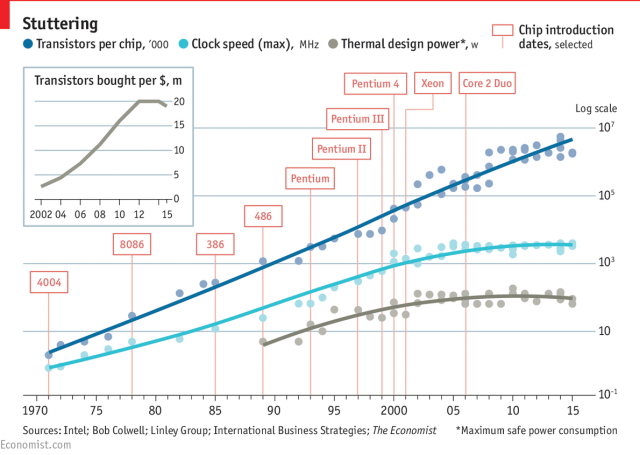
\includegraphics[width=0.7\linewidth]{MooresLaw}
  \caption[Moore's Law and the end of exponential scaling]
  {Graph of the number of transistors per chip, their clock speed, and their
  thermal design power plotted on a log scale against time. Although the number of transistors per chip
  continues to grow exponentially, the clock speed and power per chip have plateaued in the early 2000s.
  Reproduced with permission from~\cite{cross_2016}.}
  \label{fig:mooreslaw}
\end{figure}

So we've established what sorts of problems a computer can solve efficiently, and we've also noted the
exponential growth in the number of transistors on a chip. As long as both of these facts remain true, we
should only have to wait a few years before our computers become twice as powerful and problems that were
previously intractable fall within our grasp. Unfortunately, any exponential scaling must eventually fail,
and so it was for ICs for two key reasons: power and transistor size. As we made our transistors smaller,
we stopped seeing a concomitant efficiency increase, and all of a sudden, the power density of our ICs
became a limiting factor. To halt this increase, we had to reduce power dissipation, and the
only way we saw how was by capping the clock speed of our computers, which we can see in Fig.~\ref{fig:mooreslaw}
has plateaued since the early 2000s. Moreover, the smaller our transistors became, the more costly they became
to make. Even Moore's law, which has stubbornly held past the expectations of most scientists, must eventually
end as we bump up against the sizes of atoms. It seems unlikely that there is much room below Samsung's
recently announced \SI{3}{\nano\meter} node, so if we want to bring more problems into the fold of the
possible, it seems like the strong Church-Turing hypothesis must give.

It was in this context that Feynmann gave his seminal address, noting that as far as we can tell, simulating
quantum systems falls outside of the set of problems that are efficiently solveable on classical computers\cite{Feynman1982}.
However, as long as we can manipulate quantum systems, we should also be able to set up a "quantum
simulator" to see how a quantum system behaves. If this turned out to be the case, then the strong
Church-Turing hypothesis would be violated!\footnote{Despite this violation, as far as we know the original
Church-Turing hypothesis still holds. No previously uncomputable function became computable with the addition
of quantum physics.} Here was nature efficiently simulating a system that as far as we know, a Turing machine
can't. It was David Deutsch who in 1985 formalized the idea of a quantum Turing machine\cite{doi:10.1098/rspa.1985.0070},
and laid out the Deutsch-Church-Turing hypothesis, which as far as we know holds to this day:

\begin{displayquote}
  A quantum Turing machine can efficiently simulate any realistic model of computation.
\end{displayquote}

\begin{figure}
  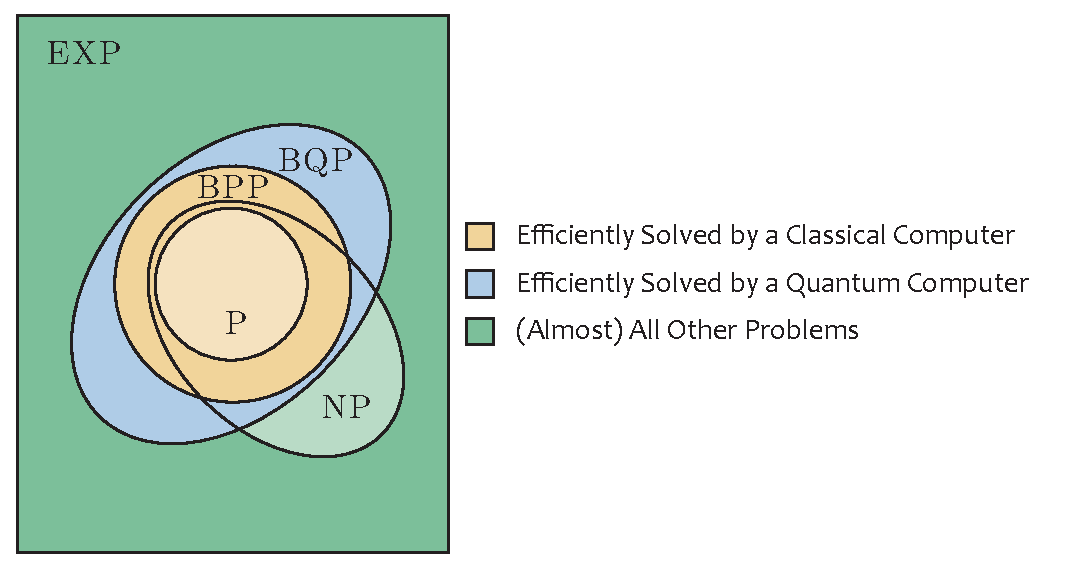
\includegraphics[width=0.85\linewidth]{ComplexityClasses}
  \caption[Relationship between various complexity classes]
  {Relationship between the various complexity classes that we've discussed. The class
  \cc{BPP} includes all problems that a classical computer can solve efficiently (including
  everything that can be calculated in polynomial time). \cc{BQP} are all problems a quantum computer can
  solve efficiently (which includes everything a classical computer can do). Finally, problems that scale exponentially
  with input size, labelled \cc{EXP}, are (almost) all other problems that are computable. The class
  \cc{NP} is also included on this figure as it is one that often comes up in the context of complexity,
  if for no other reason than to emphasize that a quantum computer \emph{cannot} solve all problems in
  this class.}
  \label{fig:complexity}
\end{figure}

With that, we finally define the class of problems that we might be able to solve efficiently if we
can build a quantum computer --- Bounded-Error Quantum Polynomial-Time or \cc{BQP}. As far as we know,
this class includes interesting problems that a classical computer could not efficiently solve. Problems
such as Shor's algorithm for prime factorization\cite{Shor} or estimating the ground state of molecules with
the Variational Quantum Eigensolver algorithm\cite{ncomms5213} have no known efficient classical algorithm
but could profoundly impact society if they are solvable. It is the promise of solutions to these problems
that drive the search for a quantum computer; however, the challenges of realizing one remain formidable. To close
out our discussion of complexity classes, I've summarized the relationship between complexity classes in
Fig.~\ref{fig:complexity}. A point I'd like to emphasize is that although \cc{BQP} is larger than \cc{P}
or \cc{BPP}, it certainly does not enclose all problems, especially those in \cc{EXP}. Although a
quantum computer may offer an exponential speedup on a subset of algorithms, it will not give us an exponential
speedup in the general case.

The remainder of this chapter aims to lay out the fundamentals of quantum computing and how we might realize
them in a semiconductor system. In Section~\ref{sec:qc} I go through a quick introduction to the concepts
underlying quantum computation. In Section~\ref{sec:qcinsm} I will detail several methods by which we might
realize a qubit in a semiconductor. Finally, in Section~\ref{sec:arch} I will examine the architectural
challenges of realizing a useful, scalable quantum computer.

\section{A Quick Introduction to Quantum Computing}
\label{sec:qc}
To build a quantum computer, we start by defining the notion of a quantum bit (qubit), which
serves as the quantum analog to the classical bit. To review, a classical \textbf{bit} is a "piece" of information
that can either take the value 0 or 1. It represents the fundamental unit of computation in digital computers.
We can take individual bits, and combine them to form a \textbf{register}, whose state is defined as
the state of each bit in the register. For example, two bits can take up to 4 different
values: 00, 01, 10, 11. Three bits can take up to 9 values, and $N$ bits can take up to $2^N$ values, however
to give the state of a register all we have to do is list the state of each bit in that register, a total of $N$ states.
By choosing various encodings of values, we can map numbers, letters, and other symbols onto these registers
and perform computations on them. For example, we can map positive integers onto registers using a base-2 number
system, as in Fig.~\ref{fig:binary}, or letters using a mapping such as ASCII, which assigns letters to 8-bit registers.
Other mappings exist for negative numbers (such as a mapping called two's complement), numbers with
decimal points (such as IEEE floating point), complex numbers and so forth.

\begin{figure}
  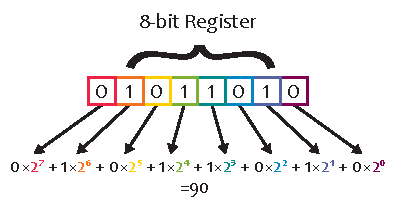
\includegraphics[width=0.75\linewidth]{Binary}
  \caption[Binary coding]
  {We can encode information in a register in many ways. One encoding for positive numbers is to use a base-2
  positional system, like above, where the binary register \texttt{01011010} is mapped to the number 90.}
  \label{fig:binary}
\end{figure}

\subsubsection{The Qubit}
A \textbf{qubit} is similar to a bit in that it has two states, $\ket{0}$ and $\ket{1}$, except unlike a bit, it is specified
by a 2-dimensional vector, and evolves according to the rules of quantum mechanics. Due to the uniquely quantum
mechanical property of \textbf{superposition}, we can no longer write the state of a single qubit (which we will
denote $\psi$) as either $\ket{0}$ or $\ket{1}$. Instead, we must write down the vector sum of the two states,
which we define as follows:
\begin{align}
  \label{eqn:basisstates}
  \ket{0} = \svec{1\\0} && \ket{1} = \svec{0\\1}
\end{align}
\begin{equation}
  \ket{\psi} = \alpha \ket{0} + \beta \ket{1} = \svec{\alpha\\\beta}
\end{equation}
where $\alpha$ and $\beta$ are complex numbers. If we were to take a measurement of this quantum state,
rather than getting back the value of this vector sum, we would measure the $\ket{0}$ state with probability
$|\alpha|^2$ and the $\ket{1}$ state with probability $|\beta|^2$. Since probabilities must sum to one, we also
get a normalization condition: $|\alpha|^2 + |\beta|^2 = 1$. The quantities $\alpha$ and $\beta$ are called
probability amplitudes, and they can take both positive and negative complex values\footnote{Interestingly, the "complex"
  part of that state is unnessecary to get the extra computing power
  of a quantum computer\cite{doi:10.1142/S0219749913500019}. There's a good reason that quantum mechanics
  uses complex probability amplitudes\cite{2004quant.ph..1062A}, but if they were real, it turns out
  we can still do computations in \textsc{BQP} efficiently.}
as long as the sum of their squared magnitudes is one. This gives us the first hint as to why quantum computing
might give us more power than a classical computer: their states can interact in a manner which mirrors
interference!

\begin{figure}
  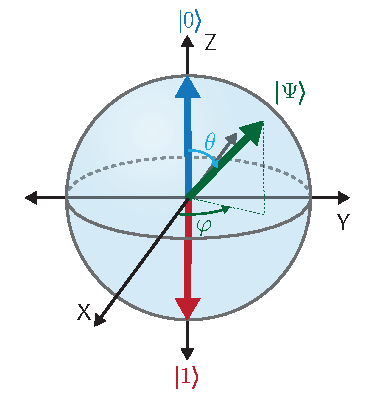
\includegraphics[width=0.5\linewidth]{BlochSphere}
  \caption[The Bloch Sphere representation of a qubit]
  {The state of a qubit can be represented as vector on the surface of a unit sphere. In this description,
  the state is described by two angles: $\theta$ and $\psi$.}
  \label{fig:bloch}
\end{figure}

Too see how this is true, it's helpful to rewrite the above state in spherical coordinates. First, let's
write $\alpha = r_0e^{-i\varphi_1}$ and $\beta = r_1e^{-i\varphi_2}$. The normalization condition is now
$r_0^2 + r_1^2 = 1$, from which we can make the replacement $r_0 = \cos(\theta/2)$ and $r_1 = \sin(\theta/2)$.
We can also factor out the phase $\varphi_1$ to give:
\begin{equation}
\ket{\psi} = e^{-i\varphi_1}\left(
    \cos\left(\frac{\theta}{2}\right)\ket{0} + e^{-i(\varphi_2 - \varphi_1)}\sin\left(\frac{\theta}{2}\right)\ket{1}
  \right)
\end{equation}
The term $e^{-i\varphi_1}$ is called a global phase factor, and is equivalent to a multiplication by a unit vector,
which it's easy to see makes no difference to the probabilities of any measurement (a fact that will continue to be
true even when we add more qubits). Another way of saying this is that the important information is encoded in
the relative phase between states. So, let's make the replacement $\phi = \varphi_2 - \varphi_1$ and ignore
the global phase factor, which gives us the state:
\begin{equation}
  \ket{\psi} = \cos\left(\frac{\theta}{2}\right)\ket{0} + e^{-i\phi}\sin\left(\frac{\theta}{2}\right)\ket{1}
\end{equation}
This representation is shown visially in Fig.~\ref{fig:bloch} and is called the Bloch sphere representation
of a qubit.\footnote{For mathematicians, this is a description of the qubit in Complex Projective Space}

Given this description, we can now start to think about what operations on a single qubit might look like.
While on a single bit, the only non-trivial operation we can perform is a flip ($0 \rightarrow 1$ and $1 \rightarrow 0$),
on a qubit we have a whole host of operations that we can perform. The only limits we put on ourselves is that these operations
must leave us on the surface of the Bloch sphere. In other words, after applying an operation, we must still
have a normalized state. From the Bloch representation, you may have already guessed that this means we
can only perform rotations.

Switching back to the 2D vector representation of a qubit, then it is also clear that these operations
must correspond to $2\times2$ matrices. The act of performing an operation corresponds to multiplying
the qubit state by one of these matrices. To ensure that the length of the qubit vector $\ket{\psi}$
remains one at all times, the matrices we can use on our qubit must be unitary. That is, given the matrix $\boldsymbol{M}$,
its complex conjugate transpose $\boldsymbol{M}^\dagger = (\boldsymbol{M^{*}})^\mathrm{T}$ times itself must be equal to
the identity matrix: $\boldsymbol{M}^\dagger\boldsymbol{M} = \boldsymbol{I}$.

Let's define three unit rotation matrices as $\pi$ rotations around the $X, Y, Z$ axes. These have the symbols
$\sigma_X, \sigma_Y, \sigma_Z$ respectively, and are called the Pauli matrices.
They have the values:
\begin{align}
  \sigma_X = \svec{0&1\\1&0} && \sigma_Y = \svec{0&-i\\i&0} && \sigma_Z = \svec{1&0\\0&-1}
  \label{eq:pauli}
\end{align}

We can build up arbitrary rotations from these unit vectors by taking various powers of these vectors
and multiplying them together. For example to apply a $\pi/2$ rotation around the y-axis applied to the state $\ket{\psi}$
we would perform $\sqrt{\sigma_Y}\ket{\psi}$. \footnote{For those familiar with the rotation operators,
this is more commonly written with a phase factor to make the solution purely real: $R_Y(\tfrac{\theta}{2})
= \exp(-i\pi/4)\sqrt{\sigma_Y}$}
A $2\pi$ rotation around the x-axis would be $\sigma_X\sigma_X\ket{\psi}$. It is possible to generalize this
to arbitrary rotations, giving us the rotation operators\cite{Nielsen:rot}:
\begin{align}
  R_X(\theta) = e^{-i \theta X/2} = \cos\left(\frac{\theta}{2}\right)\boldsymbol{I} - i \sin\left(\frac{\theta}{2}\right)\sigma_X \\
  R_Y(\theta) = e^{-i \theta Y/2} = \cos\left(\frac{\theta}{2}\right)\boldsymbol{I} - i \sin\left(\frac{\theta}{2}\right)\sigma_Y \\
  R_Z(\theta) = e^{-i \theta Z/2} = \cos\left(\frac{\theta}{2}\right)\boldsymbol{I} - i \sin\left(\frac{\theta}{2}\right)\sigma_Z
\end{align}
These three rotations (and often a global phase factor to simplify our result) are sufficient to express
any single qubit operation. For completeness, we can also define some other gates that often come up in
the context of quantum computation:
\begin{alignat}{4}
    H &=& \frac{1}{\sqrt{2}}\svec{1&1\\1&-1} &=& e^{\tfrac{i\pi}{2}} R_Y\left(\frac{\pi}{2}\right) R_Z(\pi) &=& \frac{\sigma_X+\sigma_Z}{\sqrt{2}} \\
    T &=& \svec{1&0\\0&e^{\tfrac{i\pi}{4}}}  &=& e^{\tfrac{i\pi}{8}} R_Z\left(\frac{\pi}{4}\right)          &=& \sqrt[4]{\sigma_Z} \\
    S &=& \svec{1&0\\0&i}                    &=& e^{\frac{i \pi}{4}} R_Z\left(\frac{\pi}{2}\right)          &=& \sqrt{\sigma_Z}
\end{alignat}
These are the Hadamard gate, the T gate (or $\pi/8$ gate)\footnote{The $T$-gate is often
referred to as the $\pi/8$ gate, even though it represents a $\pi/4$ rotation, a name that is derived from
the phase factor for historical reasons.} and the phase gate respectively.
As is typical, phase factors are usually dropped (something I did not do in the above), hence it is
common to see variations of these equations in the literature.

As a final example, let's take a detailed look at where interfering probabilities leads to a thoroughly
non-classical result. To start with, let's define two additional states:
\begin{align}
  \ket{+} = \frac{\ket{0} + \ket{1}}{\sqrt{2}} && \ket{-} = \frac{\ket{0} - \ket{1}}{\sqrt{2}}
\end{align}
We can get these states by starting from $\ket{0}$ and rotating $\pi/2$ or $-\pi/2$ around the Y-axis. You can
reasonably easily confirm that they are properly normalized, and that if we were to measure each state, the
probability of measuring a $\ket{0}$ or a $\ket{1}$ are equal for both states: $\mathrm{P}\left(\ket{0}\right) =
\mathrm{P}\left(\ket{1}\right) = 0.5$. So a direct measurement would be unable to distinguish these two states.
However, if we were to apply the Hadamard gate to each of those two states, we surprisingly end up with two
different outputs:
\begin{align}
  H\ket{+} = \ket{0} && H\ket{-} = \ket{1}
\end{align}
In this case, the complex probability amplitudes can interfere with each other causing the two states to
become distinguishable, something that a classical bit could not replicate. What you see is what you get.

\subsubsection{Multi-Qubit States (Qubit Registers)}
The next additional computational resource that quantum physics gives us is \textbf{entanglement}. This
resource rears it's head when we try to combine multiple qubits into a register. Formally,
we can define entanglement as a correlation between the states of qubits after they have interacted
with each other. Due to this correlation, the state of a qubit that has been entangled with its partner
can no longer be described independently, the states of the two qubits become linked. Perhaps the easiest
way to grok the consequences of this is to give an example of how this correlation might play out.

Let's start with two qubits, one of which starts in the $\ket{+}$ state, the other which starts in
the $\ket{0}$ state. If we were to apply a gate that flips the state of the second qubit if the state of
the first qubit is $\ket{1}$, then we might expect to end up with something like $\ket{+}$ in the second
qubit. If we measure the first qubit and get the result $\ket{0}$, the state of the second qubit must also
be zero, so the state of the second qubit can't have been described by $\ket{+}$. The state of the two
qubits is correlated and depend on each other. The operation we described above is called the
controlled-NOT ($CNOT$) gate, and creates a state that looks like:
\begin{equation}
  \ket{\psi} = \frac{\ket{00} + \ket{11}}{\sqrt{2}}
\end{equation}
To describe a generalized two-qubit state, we must give coefficients to each possible state the qubits
can take:
\begin{equation}
  \ket{\psi} = \alpha\ket{00} + \beta\ket{01} + \gamma\ket{10} + \delta\ket{11} =
    \svec{\alpha\\\beta\\\gamma\\\delta}
\end{equation}
So to combine two qubits together, we cannot just list the states of the two qubits one after another.
They are described by the tensor product of the two individual states: $\ket{\psi} = \ket{\psi_1}\otimes\ket{\psi_2}$.
For a three-qubit register, the total number of states we must give coefficients to is 8. For a $N$ qubit
register, the total number of coefficients is $2^N$. Note the distinction between a classical register
and a quantum register, to describe a classical register, we can list the states of the individual
bits one after another, whereas the quantum register requires $2^N$ complex numbers to express fully.

Much like a single qubit, we require new matrices that can operate on quantum registers. As one
might expect, the size of these matrices is exponential in the number of qubits that we must operate on.
For example, on a two-qubit register, we require a $4 \times 4$ matrix to describe operations. The
$CNOT$-gate that we used above is defined as:
\begin{equation}
  CNOT = \svec{1&0&0&0\\0&1&0&0\\0&0&0&1\\0&0&1&0}
\end{equation}
Unfortunately, the potential presence of entanglement means applying single or two-qubit gates to a subset
of qubits in the register is no longer a matter of applying a $2 \times 2$ or $4 \times 4$ matrix, we must
construct a $2^N \times 2^N$ matrix and apply that to the full quantum register. This construction is achieved
by taking the Kronecker product of identity matrices and the matrix we want to apply. For example, to apply
a $\sigma_X$ gate to the 2nd qubit in a three-qubit register, we construct the operator as follows:
\begin{equation}
  \sigma_{X,2} = \boldsymbol{I} \otimes \sigma_X \otimes \boldsymbol{I}
\end{equation}

The consequences of the twin effects of superposition and entanglement lead to the extra computational
power of a quantum computer, while also hinting at the difficulty of writing quantum algorithms. As we
can prepare arbitrary superposition states, we can encode an exponentially large
state into a quantum register, for example representing every number between 0 and $2^N-1$ in a $N$ qubit
register, and operate on all of these states in parallel. However, once we measure the register, we end up
with only one of the possible states in the register (i.e. the state collapses), and the quantum information
that was prepared in the state is lost. Quantum algorithms must, therefore, have three properties to be useful:
\begin{enumerate}
  \item An efficient way of preparing a state. If we want to perform computations on a quantum register
    storing $2^N$ values, we lose any exponential speedup if we need to load each of these values one-by-one.
    For example, Shor's algorithm relies on being able to prepare an equal superposition of all states
    in the register with $N$ single qubit gates\cite{PhysRevA.54.1034}.
  \item Creation of a large entangled state. Without entanglement, a quantum algorithm can be efficiently
    simulated on a classical computer. We don't know quite how to quantuntify the role that entanglement plays in computation,
    however, without using it, we know that quantum computers lose their advantage\cite{doi:10.1098/rspa.2002.1097}.
  \item A way of whittling down the quantum state to make the "answer" the likely outcome of any readout.
    Since coefficients in a quantum register represent probability amplitudes that measurement will yield
    a given outcome, we can get at most $N$ bits of data per measurement\cite{651037}, as our register
    immediately collapses into one state upon measurement. To get another value out of the register,
    we must repeat the whole computation, including loading the state.
\end{enumerate}

\subsubsection{Noise}

\begin{figure}
  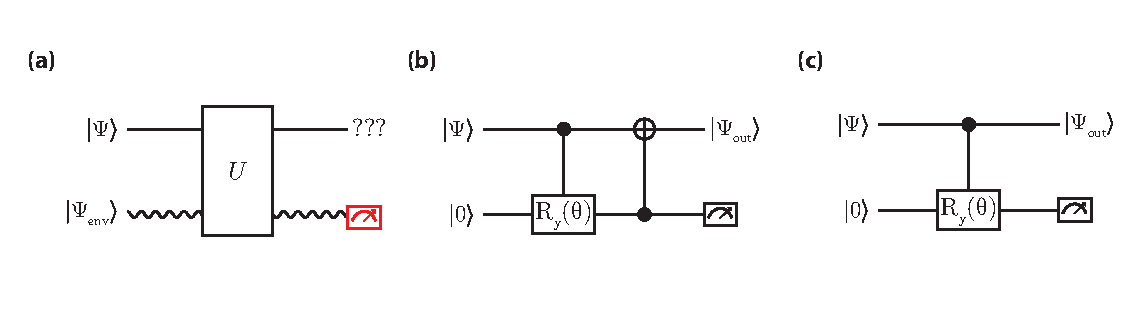
\includegraphics[width=\linewidth]{Noise}
  \caption[Noise affecting pure states]
  {(a)We can think of noise as uncontrolled interactions with an environment. However since we can't measure
  information that is transferred into the environment, we end up with an incomplete representation of our qubit.
  In order to represent this state, with some of it's information lost, we must describe the state with a density
  matrix representation. (b) A simple model for relaxation, where we represent the probability of a decay $\gamma$
  in the rotation angle $\sin^2(\theta/2) = \gamma$. Each time this gate is applied, we end up more likely to be in
  the $\ket{1}$ state. (c) A simple model for dephasing, where the phase $\theta$ is a random variable. This type
  of quantum noise has no classical analog, but causes a loss of information about the relative phase between $\ket{0}$
  and $\ket{1}$.}
  \label{fig:noise}
\end{figure}

Up to this point we have assumed that there are no noise sources or sources of information loss in our
qubit implementations. Unfortunately, reality is not so kind, and as has been discussed before, it is the
fragility of a quantum state that remains the main challenge of implementing a large scale quantum computing,
an effect called~\textbf{decoherence}. Equivalently, we can describe this effect as uncontrolled coupling to the environment, either through
energy loss or uncontrolled rotations, which leads to loss of information from our quantum computer, as shown schematically
in Fig.~\ref{fig:noise} (a), where we see a qubit $\ket{\Psi}$ interact with the environment $\ket{\Psi_{\textrm{env}}}$.
As we are unable to make a good projective measurement of the environment, the output
state after the unitary interaction $U$ with the environment cannot be well described in the vector notation we have been using
this far, and some information about the state is irrevocably lost. The challenge of including
these sources of noise into our view of quantum computing is to figure out how to model the uncontrolled environment.
\footnote{Or, we could replace the environment with something we CAN control and measure, an approach attempted
in~\cite{2018arXiv180300545M}.}
The primary way to describe such an interaction is to switch to a density matrix representation of our state, which allows us
to describe a subsystem of a composite quantum system, i.e. to ignore the portion of the state lost to the environment.
Indeed this is the most complete way to describe noise processes and information loss of our state, however rather
than introduce a more powerful and complex, but otherwise equivalent, description of quantum mechanics, we can instead model
noise processes as interactions with a controlled and known environment, such as another qubit, as in figs.~\ref{fig:noise} (b) and (c).
We can categorize interactions of our qubits into two general classes: relaxation (sometimes called amplitude
damping), and dephasing (sometimes called phase damping), which collectively lead to decoherence.

The first class of error, \textbf{relaxation}, causes our population to decay towards the ground state $\ket{0}$ each time it is
applied with probability $\gamma$. We can think about this sort of process as a loss of energy from the qubit system, and
in a way is analogous to classical relaxation, for example of an pendulum which gradually loses energy to the environment
or an atom in an excited state that decays. An equivalent circuit for such a process into a controlled environment (a second qubit) is
shown in Fig~\ref{fig:noise} (b), where the portion of the state in $\ket{1}$ undergoes a gradual rotation $R_{y}(\theta)$
towards the $\ket{0}$ state, where the phase $\theta$ is chosen to represent the probability of a relaxation event:
$\sin^2(\theta/2) = \gamma$. We represent the permanent loss of the information as a projetive measurement made on the
second qubit. This error is commonly quoted in literature as a $T_1$ time, where $T_1$ is a time constant
that gives us the rate at which a state will decay towards the ground state. Thus the probability of a relaxation event occuring
after time $t$ is given by:
\begin{equation}
  P(\ket{1} \rightarrow \ket{0}, t) = 1 - e^{-t/T_1}
\end{equation}

The second form of error, \textbf{dephasing}, is one that does NOT have a classical analog, and represents randomization of the phase between
states in the qubit or qubit register. Understanding the effect of this sort of noise is harder than for relaxation since there is no
classical analog, however if we permit ourselves a Bloch sphere representation of a qubit, we can visualize it
as a randomization of the $\varphi$ angle. An equivalent circuit, again using a second qubit to simulate the
environment is shown in fig.~\ref{fig:noise} (c). We represent an irretrievable loss of information to the
environment as a projective measurement on the second qubit. This error rate is commonly quoted as the $T_2$ time,
the rate that phase information is lost to the environment. In the case of a single qubit evolving under completely uncorrelated
(markovian) noise, this would be the end of the story, however in most systems, we also define a $T_2^*$, an ensemble
dephasing time. In the case of single qubits that evolve under quasi-static noise
\footnote{Quasi-static noise is noise that is approximately constant over the timescale of qubit operations. More formally,
we can define it as non-markovian noise, that is there is some correlation in the noise that we can learn and correct
by appropriate application of dynamical decoupling.} or multi-qubit systems that operate
under an inhomogeneous background, we can use correlations in the noise or the static nature of the inhomogeneous background
to "rephase" our qubits~\cite{PhysRev.80.580,dynamic-decoupling-biercuk}. We can think of this effect as coming from the
fact that the phase evolves at a predictable rate over the timescale of operations, such that by applying an appropriate sequence
of gates, we can unroll whatever phase was accumulated.  In this case, the $T_2$ time becomes the dephasing time after
application of rephasing gates, while $T_2^*$ is the ensemble dephasing time, assuming measurement over a longer timescale
than the correlation time and without correcting for inhomogeneities.

\section{Making Qubits in Semiconductors}
\label{sec:qcinsm}
% TODO: Add references to each of the types of qubits
Having described the basic ideas of quantum computing, our next challenge is to find a physical system that
can implement the operations that we discussed above. This problem can be distilled to that
of finding a quantum two-level system conforming to a set of criteria that were first laid out by David
DiVincenzo, criteria that are widely considered to be the standard checklist for any qubit\cite{divincenzo_crit}. They are:
\begin{enumerate}
  \item A scalable physical system with well-characterized qubits.
  \item The ability to initialize a fiducial qubit state, such that the state of the system is known prior
    to any quantum operations.
  \item Decoherence times in the qubit subspace that greatly exceed the gate operation time.
  \item A universal set of quantum gates.
  \item The ability to perform measurements on individual qubits.
\end{enumerate}
Although these criteria set out some requirements for useful qubits, they are certainly not so prescriptive
that there is a dearth of systems that could fulfil them. It is in this context that ion-trap qubits, photonic qubits,
NMR based qubits, superconducting qubits and semiconductor-based qubits are being investigated as the base of a quantum computer, each satisfying the
criteria to varying degrees. Apart from a brief discussion of the scalability prospects of each of these systems
in Section~\ref{sec:arch}, I will focus on semiconductor-based qubits for the remainder of this thesis. This type
of qubit has the potential to utilize the extraordinary processing capabilities of modern semiconductor manufacturing,
Despite narrowing the focus to semiconductor systems, there are still many
choices of two-level subspace we could use. I will not attempt to cover all the variations
of qubit that exist; rather I will focus specifically on two general designs, quantum dots and Majorana zero modes,
which in many ways share similar control and read-out. As such the discussion of physics in this section will
largely be confined to III-V materials, although I will point out that as my thesis is aimed at the general
problem of architecting a quantum computer, many of the results presented may are extensible to quantum
computers beyond spins and majoranas. Before we begin a detailed discussion of qubits in semiconductors, let's first take a look
at the physics that underlie most of these implementations; the 2-dimensional electron gas (2DEG).

\subsection{The 2-Dimensional Electron Gas}
The 2-dimensional electron gas (2DEG) is the foundation for many of the experiments and qubit-realizations to follow and
is a confinement of electrons in a semiconductor to a single plane. To fully
appreciate what this means, we first have to discuss what it means to confine an electron in one of the three dimensions.
How do we make a confining potential that can create a sheet of electrons a single electron thick? How narrow
would such a potential have to be? To answer this question, we must look at the solutions
to Schrödinger's equation in a semiconductor. These solutions will give us the distribution of the electron wavefunction, and
an idea of its "size". The following introduction is based on material taken from~\cite{delftbook, ihnbook, Ashcroft}.

\begin{figure}
  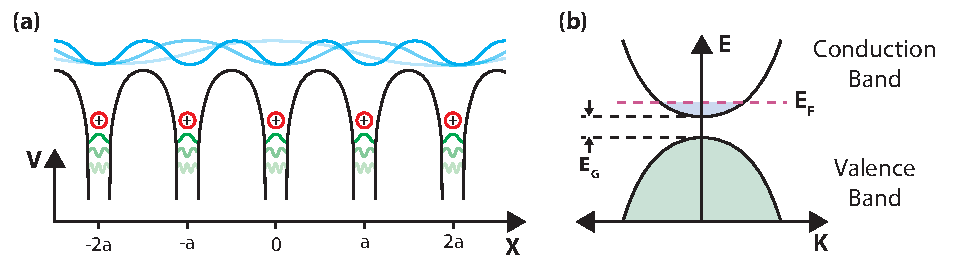
\includegraphics[width=0.9\linewidth]{BlochWaves}
  \caption[Bloch Waves on a regular lattice]
  {(a) Given a periodic lattice that creates a set of potential wells, the valid solutions for unbound
   electrons (conduction band) are plane waves with a wave vector proportional to the lattice spacing $a$,
   while solutions for bound electrons (valence band) are proportional to the strength of the potential created
   by the constituent elements of the lattice. (b) Assuming there are no electron-electron interactions,
   and the lattice may be treated as a small peturbation to plane wave solutions (the nearly-free electron model),
   the band structure will be parabolic, with a band gap $E_G$ between the valence and conduction bands, where there are
   available states. Electron states are filled to the Fermi energy ($E_\textrm{F}$).}
  \label{fig:blochwaves}
\end{figure}

In a crystalline material, such as a metal or a semiconductor lattice, we can think
about electrons as travelling through a periodic potential, caused by the periodic spacing of nuclei in the lattice, as
is shown in Fig.~\ref{fig:blochwaves}~(a) for a 1D lattice. There will be two sets of solutions; one for electrons
that are bound around nuclei which will form the valence band and one for free electron solutions which
will form the conduction band. The gap between these two solutions forms a band gap of size $(E_G)$, a range
of energies for which there are no available states. As we are looking at the 2DEG, let's focus on free electron solutions for now.
These solutions will take the form of Bloch waves, expressed as a function of lattice position $r$ and wave-vector $k$:
\begin{equation}
  \psi_{\vec{k}}(\vec{r}) = e^{i\vec{k} \cdot \vec{r}}u_k(\vec{r})
\end{equation}
where $u_k$ is a periodic function with the same periodicity as the crystal lattice and $e^{i\vec{k} \cdot \vec{r}}$ are
the general form of plane waves. What this equation effectively means is that if we are able to solve around boundary conditions for
a single unit cell, we can extract a band structure for the entire lattice.

Electrons in this system begin to fill the available states from the lowest energy up, obeying the Pauli exclusion principle which limits
each available state to two electrons with opposite spins. For conduction band electrons in uniform crystals, we can make
two additional assumptions that aid in the interpretation of the solutions to the Bloch equation. First, let's assume that
there are no electron-electron interactions. Although this assumption may at first be unintuitive, it appears
to be sufficient to describe much of the physics that follows. Second, we assume that the potential due to the
lattice is screened by valence band electrons, and can be treated as a small perturbation to a free electron. Solving
this model leads to bands which are similar to free electron plane waves up to the edge of the Brillouin zone, i.e.
up to the top of the band. In the conduction band of a semiconductor, we deal with largely empty bands, as such
the dispersion relation, i.e. the energy of electrons as a function of the wave-vector, can be approximated as that of free electrons:
\begin{equation}
  E(\vec{k}) = \frac{\hbar^2 |\vec{k}|^2}{2m^*}
  \label{eqn:3ddisp}
\end{equation}
where $\vec{k}$ is the electron wave-vector and $m^*$ is the effective electron mass that derives from the peturbation of the lattice.
The effective electron mass in this instance is a scaling factor on the increase in energy as wave-vector changes and is
defined as the curvature of the conduction or valence band of the semiconductor:
\begin{equation}
  m^* = \hbar^2 \left(\diff[2]{E}{k}\right)^{-1}
\end{equation}
Intuitively we can think of it as describing a change in momentum for a given energy "kick". For a parabolic and isotropic
band, such as for the bottom of the conduction band in a III-V semiconductor, its value is constant, however
the form of the effective mass will be more complex for materials that have directional dependences (such as Si),
or more complex band structures such as graphene. From Eqn.~\ref{eqn:3ddisp}, we can also give the
formal definition for the Fermi energy. The \textbf{Fermi energy} ($E_F$) is the energy of the highest filled electron state
at zero temperature. This situation is represented schematically in Fig.~\ref{fig:blochwaves}~(b) for a single dimension.
In 3D, the Fermi energy forms a sphere in momentum space delineating the region where electron states are filled, the surface
of which we call the Fermi surface. Finally, we can define the \textbf{Fermi wavelength} $\lambda_F$ of an electron at the Fermi
surface, effectively the size of an electron in our semiconductor. Using $k = 2\pi/\lambda$ we find:
\begin{equation}
  \lambda_F = \frac{h}{\sqrt{2m^*E_F}}
\end{equation}

\begin{table}
  \centering
  \begin{tabular}{|l|l|l|}
   \hline
   Crystal & Lattice Constant (\si{\angstrom}) & Electron Effective Mass$(m^*/m_e)$ \\
   \hline
   Si & 5.43 & - \\
   Ge & 5.658 & - \\
   GaAs & 5.65 & 0.066 \\
   InAs & 6.06 & 0.026 \\
   InSb & 6.48 & 0.015 \\
   \hline
  \end{tabular}
  \caption[Properties of some common Semiconductors]
  {Lattice constants and effective electron masses for some common semiconductors. For Si and Ge semiconductors, which are
  indirect band gap semiconductors, the effective mass for electrons is not trivial and will vary based
  on direction and valley state, hence values are not given above. Values are taken from~\cite{Kittel2004,InSbParam}.}
  \label{tab:semiprop}
\end{table}

If we wish to confine electrons in a given dimension, the Fermi wavelength gives us the length-scale on which we must form
our confining potential. For metals, the large number of free electrons means the Fermi energy is large, and as such we end up with a
Fermi wavelength on the order of a few Ångström (where $\SI{1}{\angstrom} = \SI{1e-10}{\meter}$). In semiconductors, as
the number of free electrons, and hence the Fermi energy, is set by the doping and is generally small, the Fermi
wavelength can be on the order of a few 10s of nanometers. Parameters for some common semiconductors are given
in Table~\ref{tab:semiprop}. Given these values, if we can make a potential well with a width $W$ that's on
the order of the Fermi wavelength, we can confine electrons to a few subbands. The next question is: how
do we create a narrow quantum well?

\begin{figure}
  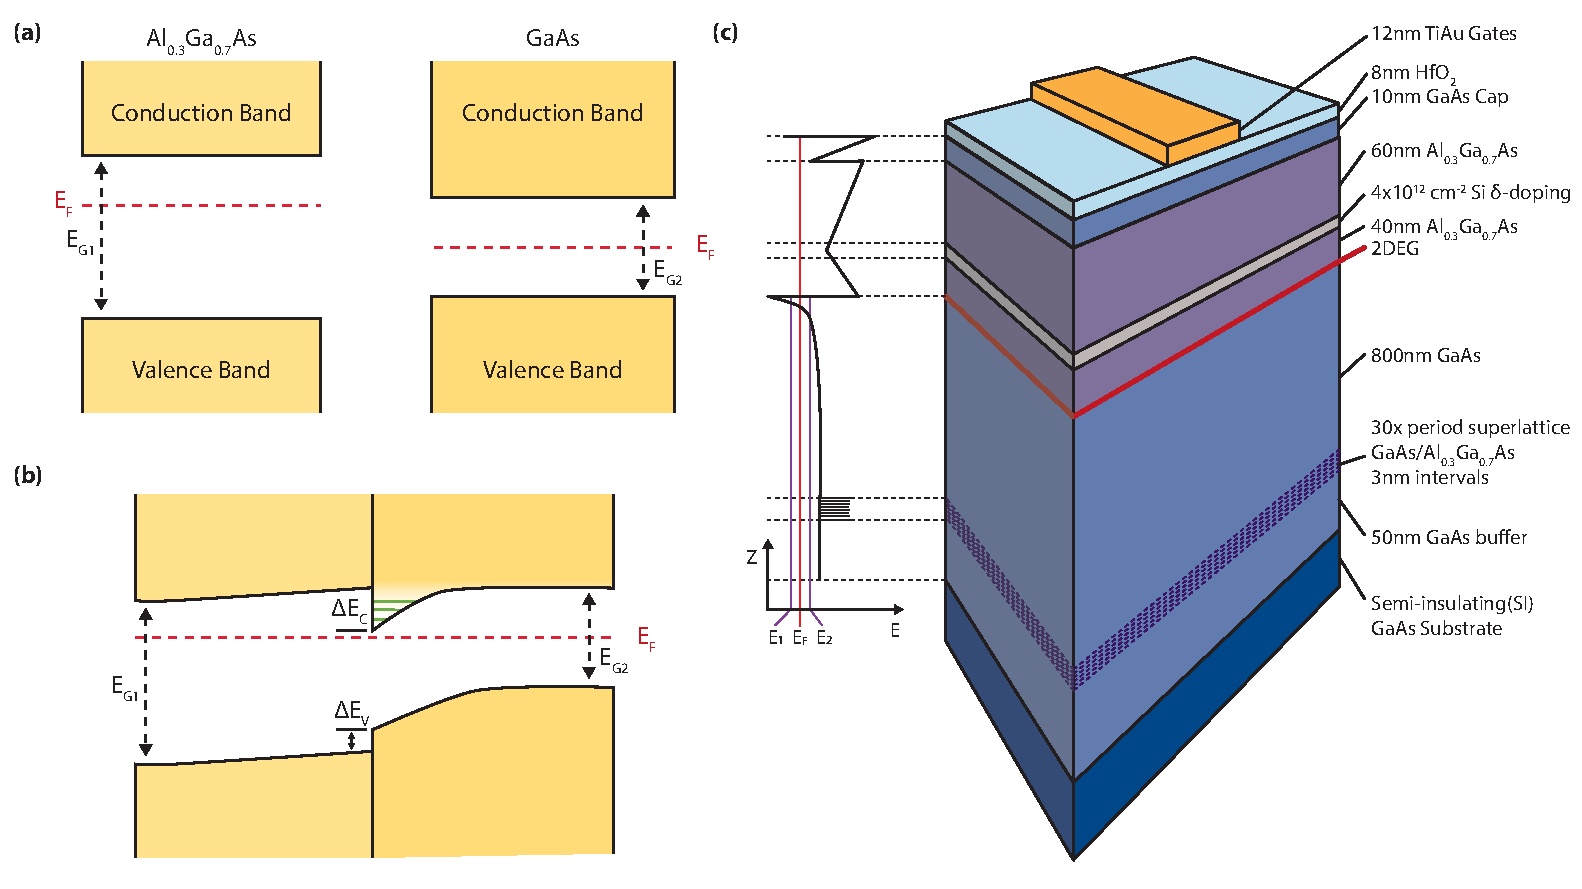
\includegraphics[width=1\linewidth]{GaAs}
  \caption[Band bending in a straddling type heterojunction, and the GaAs/AlGaAs heterostructure]
  {\label{fig:heterostructure}(a) Shows a straddling type heterojunction between \ce{Al_{0.3}Ga_{0.7}As} and GaAs with two
  differing bandgaps $E_{G1}$ and $E_{G2}$, where the smaller gap ($E_{G2}$) is fully enclosed in the larger gap $E_{G1}$.
  (b) When the two semiconductors are equalized, their bands bend near the heterojunction to ensure a continuous Fermi energy.
  Far from the junction, the unmodified band structure is restored. (c) The layer stack of a GaAs/(Al,Ga)As heterostructure,
  with TiAu surface gates that can locally modify the density of the 2DEG.}
\end{figure}

The answer is to create a heterojunction; an interface between two dissimilar semiconductors with different band-gaps.
The simplest type of heterojunction we can form is a straddling (type I) junction, where one semiconductor has a smaller band-gap
that is contained within the band gap of the other, a situation that is represented schematically in Fig.~\ref{fig:heterostructure} (a).
In the case that the Fermi levels of the two semiconductors are unequal, electrons tunnel through the junction to align
their levels, leading to band bending at the interface. Careful choice of semiconductors can cause a well to appear at the interface,
where the width of the well can be designed to be on the order of the Fermi wavelength in the semiconductor. GaAs and (Al,Ga)As are
an ideal choice for this type of heterojunction as they are almost perfectly lattice matched (their lattice constants differ by 0.14\%),
while also forming a straddling-gap heterojunction. The gap in GaAs is $E_{G1} = \SI{1.424}{\electronvolt}$ and the gap in
\ce{Al_{1-x}Ga_{x}As} can be continuously varied by
changing the ratio of Al and Ga in the semiconductor, taking the value $E_{G2} = 1.424 + 1.225x$ \si{\electronvolt}.
Furthermore, up to $x = 0.44$, the ratio of the step in the conductance
band ($\Delta E_C$) to the step in valence band ($\Delta E_V$) is a constant: $\Delta E_C/\Delta E_V = 1.5$~\cite{adachi1993properties}
[see steps in Fig.~\ref{fig:heterostructure}~(b)], allowing the depth of the well to be easily varied.
Finally, by doping the semiconductor with Si, we can move the Fermi energy up to populate a single subband, leading to a
2-dimensional plane of electrons, where there is only a single wave-vector in the Z direction ($k_z$) that electrons can take. As long
as the electron temperature is far below the energy gap of the subbands, only this subband will be populated.

The structure of a typical GaAs/\ce{Al_{0.3}Ga_{0.7}As} heterostructure is shown in Fig.~\ref{fig:heterostructure}~(c). Such structures
are normally grown by molecular-beam epitaxy (MBE) which allows atomically smooth layers to be grown a single monolayer
at a time. We start with a semi-insulating GaAs substrate, over which a large buffer is grown.
Repeated thin layers of GaAs/\ce{Al_{0.3}Ga_{0.7}As} are grown to reduce the dislocation density
and create a continuous, smooth single crystal at the heterojunction, and to trap impurities which may percolate upwards
during the annealing stage of the growth. The red line represents the 2DEG itself on the schematic,
followed by a region of Si $\delta$-doping, used to pin the Fermi level in the substrate, and
a \SI{10}{\nano\meter} GaAs cap to protect against oxidation. During processing, a protective oxide barrier
(either \ce{HfO2} or \ce{Al2O3}) is grown, followed by surface gates which allow the density of states to be locally modified, or even depleted,
to define structures in the 2DEG. The oxide layer, apart from serving as a passivation barrier, is also necessary to
prevent tunnelling of electrons from the surface gates into the donor layer, where the movement of electrons is known to be a significant
source of charge noise~\cite{PhysRevB.72.115331, PhysRevApplied.9.034008}.

Having confined electrons into 2-dimensions, we can now redefine several of the parameters that we had above. First, our
dispersion relation becomes that of free electrons in two-dimensions:
\begin{align}
  E(\vec{k}) = \frac{\hbar^2 |\vec{k}|^2}{2m^*} && |\vec{k}|^2 = k_x^2 + k_y^2
  \label{eq:k2d}
\end{align}

We can also define the density of states (DOS) in 2-dimensions as the number of states $n(E)$ per unit energy $(E)$:
\begin{equation}
  \rho_{2D} = \diff{n(E)}{E}
\end{equation}

For free electrons in 2D, the states fill an area in momentum-space up to k-vector $k$:
\begin{equation}
  A = \pi k^2 = \frac{2 \pi m^* E}{\hbar^2}
\end{equation}
where we've substituted equation~\ref{eq:k2d} for $k$. The spacing of states in a crystal of size $L \times L$ is given
by $\pi^2/4 L^2$, so for a unit area, the area of a single state is $A_{\textrm{single}} = \pi^2/4$. Putting this together,
the number of states up to energy $E$ is therefore:
\begin{equation}
  n(E) = g_s g_v \frac{A}{A_{\textrm{single}}} = g_s g_v \frac{m^* E}{2 \pi \hbar^2}
\end{equation}
and giving a density of states:
\begin{equation}
  \rho_{2D} = g_s g_v \frac{m}{2 \pi \hbar^2}
\end{equation}
where $g_s$ is the \textbf{spin degeneracy} (almost always 2), and $g_v$ is the \textbf{valley degeneracy} (1 for III-V semiconductors, 3 for Si).
Importantly we note that the density of states is independent of energy, a situation which is unique to 2-dimensions.
Finally, we redefine the Fermi energy, wave-vector and wavelength in terms of the total electron density ($n_s$), which give the following equations:
\begin{align}
  E_F = \frac{n_s}{\rho_{2D}} = \frac{2 \pi \hbar^2 n_s}{m^* g_s g_v} &&
  k_F = \sqrt{\frac{4 \pi n_s}{g_v g_s}} &&
  \lambda_F = \sqrt{\frac{\pi g_s g_v}{n_s}}
\end{align}

Having detailed the formation of 2DEGs, we must now consider the factors that will affect their quality for
experimental purposes. Broadly, the two most important effects that will affect the quality of the
2DEG are temperature and scattering. First, the main effect of temperature will be to create a distribution of filled states around the Fermi energy, rather
than a sharp cut-off as we had previously assumed. This distribution is called the Fermi-Dirac distribution and takes the form:
\begin{equation}
  f(E - E_F) = \left[1 + \exp\left(\frac{E - E_F}{k_B T}\right)\right]^{-1}
\end{equation}
This thermal population places an additional constraint on 2DEG formation, namely that the thermal energy $k_B T$ should be much less than the
2D subband spacing, a requirement that is easily met for most heterostructures below a few Kelvin. Second, we account for the
effect of scattering, which we capture in the form of a length that an electron can travel before scattering. Depending on the scattering
mechanism this can either be inelastic, normally due to scattering off phonons (thermal scattering), or elastic, normally due to
scattering off lattice defects or impurities. Therefore we define two length scales, $l_\psi$ being the inelastic scattering length,
which gives us the length scale over which total kinetic energy and momentum are conserved, and $l_e$ being the elastic scattering
length, which gives the length of time an electron will travel before any collision. From this, we can also define the momentum relaxation time, the
amount of time between electron collisions, given by $\tau = l_e/v_F$.

In general, we are more interested in the effect of scattering on conductivity, an easily measured bulk property of
the semiconductor. We can reframe the scattering time into a conductivity by considering the motion of an electron
through a lattice. Let's define a quantity called the drift velocity $v_d$ as the average speed an electron moves through
the lattice under an accelerating field $E$. Then, by Newton's second law:
\begin{equation}
  eE = \frac{m^* v_d}{\tau}
\end{equation}
If we rearrange for $v_d$ we find:
\begin{align}
  && v_d = \mu E && (\textrm{where~} \mu = \frac{e \tau}{m^*})
\end{align}
where $\mu$ is a quantity called mobility, with units \si{\square\centi\meter\per\volt\per\second}.
To find the conductivity, we remember the definition for current
density, which will be given by the number of electrons that pass an area per second, $J = n_s e v_d$,
and the definition of conductivity, which is simply the current density per electric field, $\sigma = J/E$. From here,
we find the equation for conductivity in terms of electron density and mobility to be:
\begin{equation}
  \sigma = n_s e \mu
\end{equation}

At this point, our discussion splits into two streams.
The first deals with the formation of quantum dots, structures with tight confinement in all three dimensions,
and is covered in Section~\ref{sec:qd}. The second deals with the characterization of 2DEGs, extracting
the mobility, density, strength of the spin-orbit interaction, via weak (anti-)localization measurements and the quantum
Hall effect, and is covered in Section~\ref{sec:char}. Both of these are crucially important for building a variety of
qubits in semiconductors, and many of the advances in both spin qubits and topological qubits stem
from improvements in materials science that have led to higher quality 2DEGs and the availability of exotic material systems.

\subsection{Quantum Dots}
\label{sec:qd}
Let's now consider the question of how we might use the 2DEG to form a qubit. This can occur in many different
ways, for example through the creation of superconducting Josephson junctions with a 2DEG to tune the Josephson
energy~\cite{karl-gatemon} or in Majorana zero modes\cite{PhysRevLett.119.136803}, formed using a 2DEG as a starting
point, a topic we shall explore in Section~\ref{sec:majo}. By far the most well studied 2DEG based qubit is the zero-dimensional
quantum dot, used to confine electrons using surface gates to define zero-dimensional "puddles" of electrons
~\cite{RevModPhys.79.1217,RevModPhys.75.1}.
These puddles of electrons, which in a semiconductor have dimensions on the order of the Fermi wavelength $\lambda_F$,
creates a discrete spectrum of available states, a situation akin to having an atom with a set of orbital modes
defined in the middle of your 2DEG\cite{PhysRevLett.77.3613}. Before considering a quantum dot in a semiconductor, let's
start by looking at a small metal island, which will not have well resolved orbital modes but can still contain a discrete,
well defined, number of electrons.

\begin{figure}
  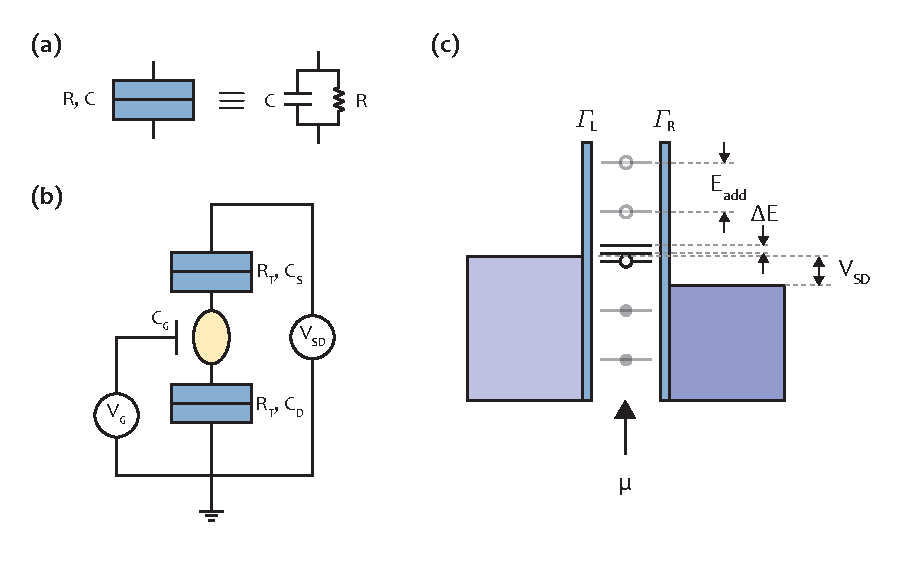
\includegraphics[width=0.8\linewidth]{Dot}
  \caption[Schematic of a single quantum dot]
  {\label{fig:QD}(a) We define a tunnel junction as a combination of a resistor and a capacitor in parallel
  since for a quantum dot the geometric capacitance of the junction is significant. (b) Equivalent circuit
  model of a quantum dot. The dot is connected to reservoirs by a source and drain tunnel junction, where
  we define the drain as ground. A voltage $V_SD$ may be applied across the quantum dot, which may cause current
  to flow. The levels of the quantum dot can be tuned by a gate voltage $V_G$ that is capacitively coupled to the
  quantum dot. (c) Schematic of a quantum dot showing a "ladder" of states, and orbital energy level. When a level
  falls within the source-drain bias window current may flow across the dot, otherwise current is blocked, an
  effect termed Coulomb blockade.}
\end{figure}

To understand how this is possible, we begin with the formula for the energy on a capacitor, the same one that
we initially give for a classical capacitor. This is given by: $E = Q^2/2C$. The energy to add a single extra electron
to this island is the \textbf{charging energy}:
\begin{equation}
  E_C = \frac{e^2}{2 C_{\Sigma}}
\end{equation}
where $C_\Sigma$ is the total capacitance to the dot. We then couple this island to two reservoirs, say a source
and a drain, both with resistance $R_t$. Realistically, these coupling resistances each add a capacitance term, which
we must consider in our $C_\Sigma$ term, as shown in Fig.~\ref{fig:QD} (a). We can also add a gate nearby that we can use to pull electrons on and off
the island. This situation is represented schematically in Fig.~\ref{fig:QD} (b). You might ask what differentiates
this system from a circuit I could make on my bench with three capacitors and two resistors. In other words, what are
the conditions for the number of electrons on the dot to be well defined? Firstly, we want the thermal energy
in the system to be much smaller than the charging energy; otherwise, we won't have a well-defined ground state:
\begin{equation}
  k_B T \ll E_C
\end{equation}
Next, we want to ensure that tunnelling occurs at a slow rate relative to the Heisenberg uncertainty relation
$\Delta E_C \Delta t \geq h/2$. If this condition is not met, dots can hop on and off the dot faster than we could resolve them.
The tunnelling time is given by $\tau = R_t C$, the time constant of the system. Combining $\tau$ and $E_C$,
we derive our second restriction:
\begin{equation}
  R_t \gg h/e^2
\end{equation}
This quantity $h/e^2$ is called the von-Klitzing constant, or the quantum or resistance, and will show up
throughout this thesis in several contexts; as the resistance of a 1D channel, the resistance of an edge
state in the quantum Hall and spin quantum Hall effect and the tunnelling rate through coupled Majorana zero modes,
and has the value $R_K = \SI{25812.807}{\ohm}$.

From here, we can define the total energy of the quantum dot with $N$ electrons. To do this, we will use a
semi-classical model called the constant-interaction model. This model defines the energy in terms of the background charge $N_0$, and
\footnote{We can think of the background charge $N_0$ as the quantized equivalent of the Fermi energy. It is equivalent
to $E_F = N_0^2 E_C$, and tells us how many electrons are in the dot at zero gate voltage.},
the voltage and the capacitance of the source, drain, and gate. At this point we can work in the limit of
a small-sized dot relative to the Fermi wavelength, and reintroduce the orbital energy levels $E_n(B)$. Here $E_n(B)$
is defined as the energy of the $n$-th orbital under a magnetic field B. This gives the equation for total energy of the quantum
dot as:
\begin{equation}
  U(N) = \frac{[-|e|(N-N_0) + C_SV_S + C_DV_D + C_GV_G]^2}{C_\Sigma} + \sum_{n=1}^{\left\lfloor\frac{N}{g_sg_v}\right\rfloor} E_n(B)
\end{equation}
Note that we've included the spin and valley degneracies in the filling of the orbital states of the quantum dot in
the summation of $E_n(B)$. We can also define the electrochemical potential $\mu(N)$ of the dot:
\begin{multline}
  \mu(N) \equiv U(N) - U(N-1) \\
    = \left(N - N_0 - \tfrac{1}{2}\right)E_C - \frac{E_C}{|e|}\left(C_SV_S + C_DV_D + C_GV_G\right) + E_{n}(B)
  \label{eqn:onemu}
\end{multline}
Note that we've assumed that we are tunnelling into the lowest unoccupied orbital energy level $E_n$. It is a reasonably
simple modification to Equation~\ref{eqn:onemu} to calculate the chemical potential of tunnelling into an excited orbital
state. The most important difference between the chemical potential $\mu$ and the energy $E$ is the linear dependence on gate voltage,
which allows us to draw a "ladder" of states where the gap between each state is a fixed value:
\begin{equation}
  E_{\textrm{add}}(N) = \mu(N+1) - \mu(N) = E_C + \Delta E_n
\end{equation}
This is depicted schematically in Fig.~\ref{fig:QD} (c). This equation also shows us that the electrochemical
potential of the dot can be swept linearly by varying the gate voltage.

\begin{figure}
  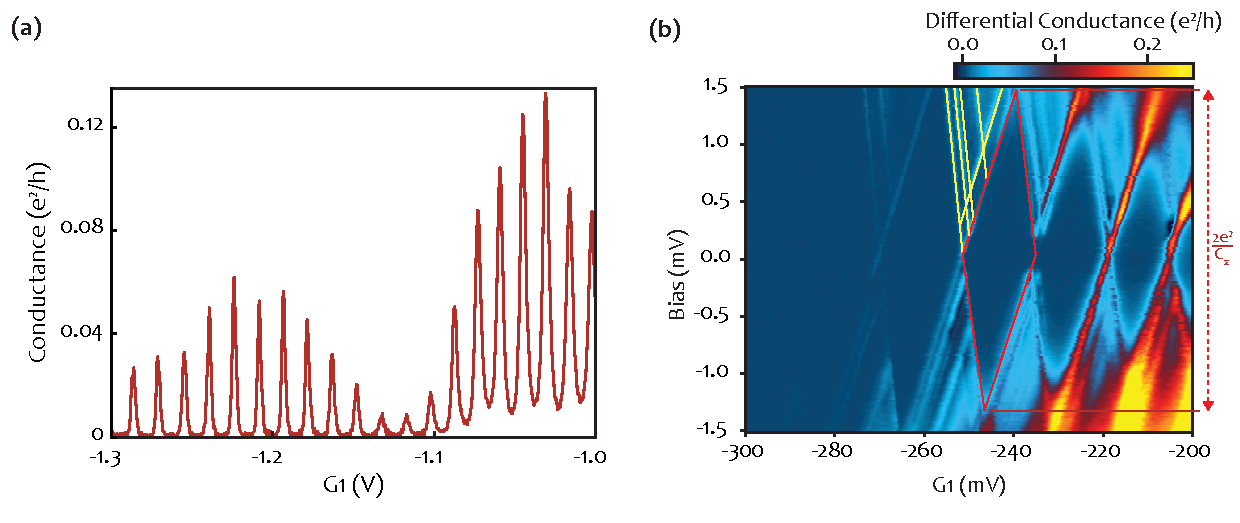
\includegraphics[width=1.0\linewidth]{CB}
  \caption[Coulomb Blockade in a single quantum dot]
  {\label{fig:cbtrans}(a) Coulomb Blockade through a single quantum dot. Current can only flow at points
  where the energy levels in the dot are in alignment with the reservoirs, which occurs as the gate voltage
  is swept. (b) Sweeping bias as well as the gate, we get diamond-like features as the levels move into
  and out of the bias window. The charging energy can be extracted by looking at the width of a diamond, as
  shown in red, and increases as the size of the dot is reduced by a more negative confining potential. We can
  also see excited states within each diamond, highlighted in yellow on a single diamond. These correspond to orbital
  modes within the quantum dot.
  }
\end{figure}

The next question we might ask is: how can we flow current through the dot. Current can only flow via the addition of an electron
from the source ($N \rightarrow N+1$) and the removal of an electron to the drain ($N+1 \rightarrow N$), which only occurs
when the electrochemical potential $\mu(N)$ falls within the source-drain window of the reservoirs for some N:
\begin{equation}
  E_F - \frac{|eV_{SD}|}{2} \leq \mu(N) \leq E_F + \frac{|eV_{SD}|}{2}
\end{equation}
This leads to a peaked conductance spectrum at low source-drain bias as a gate voltage is swept (as in Fig~\ref{fig:cbtrans} (a)), or
diamond-like regions of blocked conductance as source-drain bias is swept as a function of gate voltage (as in Fig~\ref{fig:cbtrans} (b)),
an effect termed Coulomb blockade. The spacing of Coulomb diamonds allows the extraction of charging energies and addition energies, as
well as the lever arm $\alpha$. This is the ratio of gate capacitance to total capacitance for each gate that is swept. The width of Coulomb
peaks reveals information about the temperature of the electrons, as high electron temperatures smear the population in
the source and drain reservoirs. I do not give a derivation of this effect here; however, we point the curious reader to~\cite{grabert2013single},
and note that this is the method by which we extract electron temperatures in Section~\ref{sec:gb_paper}.

\subsubsection{Double Quantum Dots}
\begin{figure}
  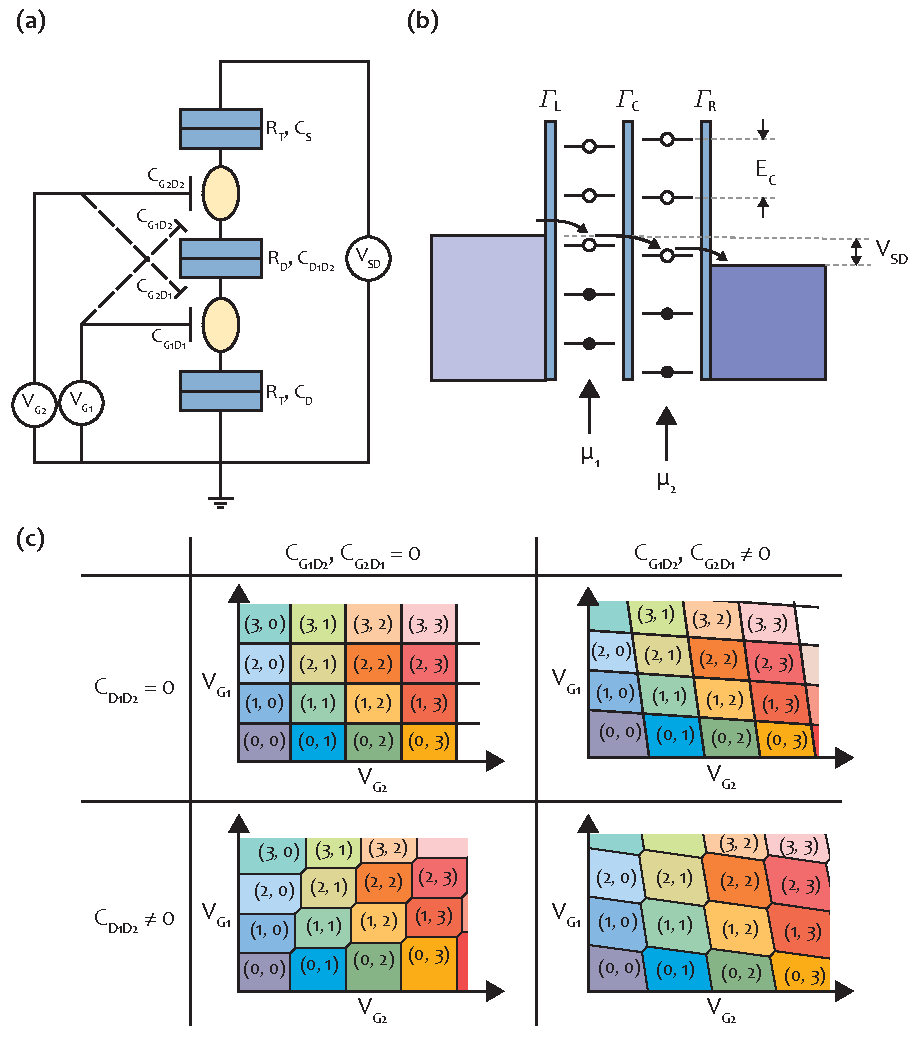
\includegraphics[width=1.0\linewidth]{DoubleDot}
  \caption[Schematic of a double quantum dot]
  {\label{fig:dqd}(a) Equivalent circuit model for a double quantum dot. The circuit is very similar to that of
  two single quantum dots in series, except that we must also account for cross capacitances between adjacent gates
  (the terms $C_{G1D2}$ and $C_{G2D1}$), as well as the contribution of the tunnel junction between the left and
  right dots (the term $R_D$ and $C_{D1D2}$). (b) Energy levels in a double quantum dot system. For current to flow
  through this circuit, there must be an available level in both the left and right quantum dots. (c) Here we map
  out the effect of cross capacitance and inter-dot capacitance on the charge stability diagrams of a double quantum
  dot system as $V_{G1}$ and $V_{G2}$ are varied. As each $V_{G1}$ ($V_{G2}$) becomes more positive, more dots are
  pulled onto the left (right) quantum dot. If gate capacitance is non-zero, the lines take on a slope. If inter-dot
  capacitance is non-zero, each stable configuration splits into a hexagonal cell. Note that these drawings do
  not include the effects of tunnelling between dots.}
\end{figure}

Before we move onto a discussion of how we might use these to form qubits, I will introduce the double quantum dot,
where we couple two single dots together. Much like we can consider a single quantum dot an
artificial atom, so too we can consider two quantum dots that allow tunnelling of electrons between each side as
an artificial molecule. The extension of the single quantum dot picture to a double quantum dot picture occurs by
adding a tunnel junction between the left and right dots, and adding a gate to control the
electrochemical potential of the second quantum dot, as shown in Fig.~\ref{fig:dqd} (a).
To completely model the effect of a double quantum dot, we must account for two additional sources of capacitance, first
a cross-capacitance between the left (right) gate and the right (left) quantum dot, and second the capacitance between
the left and right dot. Intuitively we can understand the capacitance between dots as a new electron on the left dot
shifting the energy and chemical potential of the right dot or vice-versa, leading to a shift in the locations of charge
transitions as electrons are pulled on and off each quantum dot. To characterize the effect of the two gates on a double
quantum dot, we can plot the ground state occupancy of the quantum dots as each of the gate voltages is swept, in a plot
called a charge stability diagram. A mockup of charge stability diagrams are shown in Fig.~\ref{fig:dqd} (c) as both interdot
capacitance and gate cross-capacitance are turned on and off. The occupancy of the double quantum dots is labelled
$(N, M)$ where $N$ represents the occupancy of the left double quantum dot and $M$ represents the occupancy of
the right double quantum dot.

As with a single quantum dot, we can define the energy of the double quantum dot system using the constant
interaction model:
\begin{multline}
  U(N, M) = \frac{[-|e|(N-N_{0}) + C_SV_S + C_{G1D1}V_{G1} + C_{G2D1}V_{G2} - |e|MC_{D1D2}]^2}{C_{\Sigma,1}} \\
          + \frac{[-|e|(M-M_{0}) + C_DV_D + C_{G1D2}V_{G1} + C_{G2D2}V_{G2} - |e|NC_{D1D2}]^2}{C_{\Sigma,2}} \\
          + \sum_{n=1}^{\left\lfloor\frac{N}{g_sg_v}\right\rfloor} E_{n,1}(B)
          + \sum_{m=1}^{\left\lfloor\frac{M}{g_sg_v}\right\rfloor} E_{m,2}(B)
\end{multline}
where we have added terms $C_{G1D2}$ and $C_{G2D1}$ to represent the cross capacitance between opposite
gates and dots, and $C_{D1D2}$ is the capacitance between dots. The electrochemical potential for each dot
can also be defined in a similar way:
\begin{align}
  \mu_1(N, M) \equiv U(N, M) - U(N-1, M) \\
  \mu_2(N, M) \equiv U(N, M) - U(N, M-1)
\end{align}

\begin{figure}
  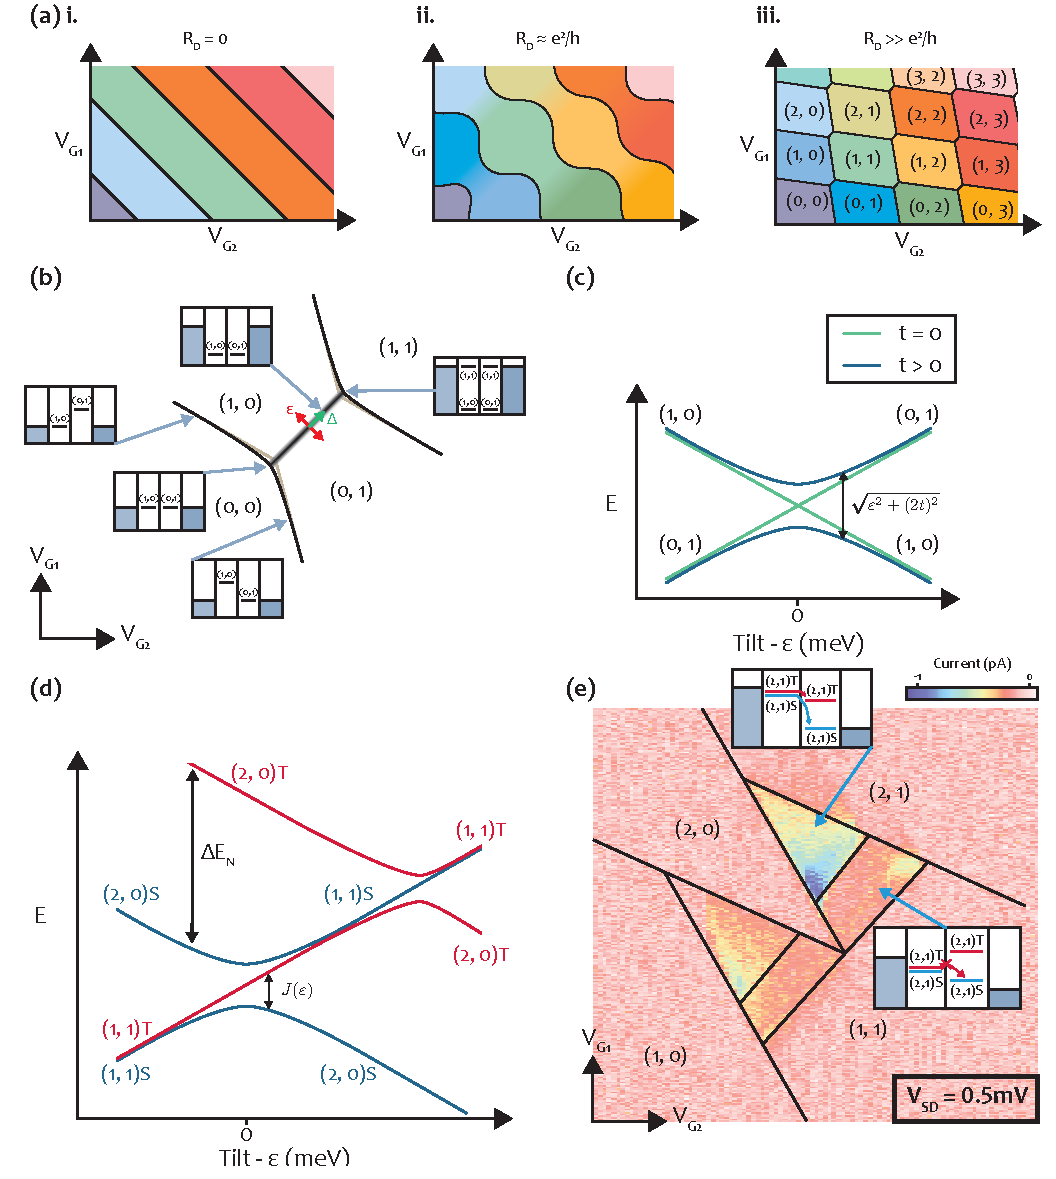
\includegraphics[width=0.9\linewidth]{ddenergy}
  \caption[Energy levels and spin in a double quantum dot]
  {\label{fig:dqdenergy}(a) Effect of varying $R_D$, the tunnelling rate between the two
  dots. At low resistance, the dot effectively reverts to a single quantum dot. As the resistance is increased towards
  $e^2/h$, two separated dots begin to form, although the transition between them is tunnel broadened.
  Finally, if the resistance is much larger than $e^2/h$, there are well defined transitions between left and right
  dot. (b) Zoom up of a single honeycomb cell around the $(0, 0)$, $(1, 0)$, $(0, 1)$ and $(1, 1)$ charge transitions.
  Insets show energy levels $\mu_1(N, M)$ of the left quantum dot and $\mu_2(N, M)$ of the right quantum dot where bracketed
  numbers indicate the charge occupancies of both dots. We define the tilt (offset) axes perpendicular (parallel) to the
  inter-dot transition in red (green). (c) Calculated energy levels along the $(0,1) \rightarrow (1,0)$ charge transition according
  to a full quantum model. For finite tunnel coupling, an avoided crossing is formed. (d) Calculated energies of singlet and
  triplet spin configurations for a two-electron double quantum dot. Due to the Pauli exclusion principle,
  the $(2, 0)T$ state is not accessible until we reach the first excited orbital state, such that the $(2, 0)T$ level is energetically
  inaccessible at zero tilt. We define the exchange energy $J(\varepsilon)$ as the energy between the $(1, 1)S$ and $(1, 1)T$
  states. (e) Current through a double quantum dot at $V_{SD} = \SI{0.5}{\milli\volt}$. Charge transitions split into finite bias triangles
  which reveal the presence of excited orbital states in the dot, as well as the effects of spin, which blocks transport through the orbital ground state of the dot.}
\end{figure}

The constant interaction model, however, has limited power to describe the effects of tunnelling between two dots,
as it assumes that the occupancy of each dot is a good quantum number, a situation which will not hold near
charge degeneracy points, specifically when tunnelling rates between the two dots is significant. If we wish to include a finite tunnel
rate, we must move to a Hubbard model that includes the effects of quantum fluctuations, spin and orbital states on each
dot~\cite{PhysRevB.84.115301}. In this model, and indeed in most descriptions of double quantum dots, we
describe the strength of tunnelling between the two quantum dots as a \textbf{tunnel coupling}. This model allows us to draw a schematic
of the continuous evolution from a single quantum dot to a double quantum dot as the strength of the inter-dot tunnel coupling
is increased. For example, in Fig.~\ref{fig:dqdenergy} (a) we see the evolution from the case with large tunnel coupling (~zero tunnel resistance), i.e. a single
quantum dot in i., to a region of intermediate tunnel coupling in ii., and finally small tunnel coupling, i.e. a wholly separated quantum dot, in iii. In the
limit of smaller tunnel couplings (larger tunnel resistance), the bending of charge transitions will continue to be visible
at each charge transition as in Fig~\ref{fig:dqdenergy} (b), where the transitions of the constant interaction model (grey) are compared to
a full hubbard model (black).

We can examine in further detail a single honeycomb cell in the charge stability diagram of a dot that includes both a cross-capacitance and an inter-dot capacitance.
In the insets of Fig~\ref{fig:dqdenergy} (b) we map out the energy levels of a quantum dot at various points according to the constant interaction model.
In this case, looking at the $(0, 0), (0, 1), (1, 0), (1, 1)$ transition, we find two points where
three charge transitions meet, so-called triple points, where energy levels within both the left and right dot are aligned
with the reservoirs. If we were to try and pass a current through such a system, it would only be at these points that a
current would flow. In between these triple points we find a new inter-dot transition, which comes from the fact that $\mu_{(1 \textrm{~and~} 2)}$
is now a function of gate voltage \emph{and} the occupancy of dot $(2 \textrm{~and~} 1)$. This dependence on the
occupancy is a result of the inter-dot capacitance and leads to an additional penalty that must be
overcome to load an electron on both left and right dots. Hence, the point where we move to the $(1, 1)$ charge configration is
pushed up in both $V_{G1}$ and $V_{G2}$, and a $(0, 1) \rightarrow (1, 0)$ interdot transition appears. To further analyze this charge transition,
we rotate ourselves to align with the inter-dot transition and define two new perpendicular axes.
Tilt ($\varepsilon$) is defined as movement perpendicular to the interdot charge transition and is shown in red. It measures the relative
charge configuration of the dots ($\varepsilon = \mu_1 - \mu_2$) while keeping the overall charge of the two dots constant.
Offset ($\Delta$) is defined as movement parallel to the interdot charge transition and is shown in green.
It measures the total charge offset $\Delta = \mu_1 + \mu_2$ without modifying the relative distance between levels in the left
and right dot. In this way, we can move through the charge stability diagram in a way that ignores the effects of cross capacitances~\cite{qubyte}.

Having defined the tilt axis, we can analyze in detail the inter-dot charge transition, which for moderate tunnel couplings will show
charge hybridization near the interdot charge transition. At these points, the charge becomes a bad quantum number and electrons become delocalized
across the two quantum dots, leading to a blurred charge transition [as sketched in Fig~\ref{fig:dqdenergy} (a) ii.]. If we calculate the energy
of the two charge states along the tilt axis, plotted in Fig.~\ref{fig:dqdenergy} (c), we find that a finite tunnel coupling leads to the
formation of an avoided crossing (blue), compared to no tunnel coupling (green), which at the centre will have a gap of $2t$. As a function of
tilt, we find the difference in the gap between the two states is:
\begin{equation}
  \Omega(\epsilon) = \sqrt{\varepsilon^2 + (2 t)^2}
\end{equation}
The charge hybridization also allows the measurement of tunnel coupling by measurement of the charge state near zero tilt,
which for intermediate tunnel couplings will vary smoothly between $(0, 1)$ and $(1, 0)$~\cite{PhysRevLett.92.226801}.

\subsubsection{Spin}
The final effect we must include to describe the relevant physics is spin. Electrons are fermions, meaning
they have half-integer spin and obey the Pauli exclusion principle, an effect we've run into before when we considered
the filling of bands in a semiconductor. As a quick reminder, the spin of a system is described by the spin angular momentum operator
$S = [S_x, S_y, S_z]$ and a spin magnitude (principal spin) operator $S^2 \equiv S_x^2 + S_y^2 + S_z^2$. The three orthogonal projections of the spin
angular momentum are non-commuting, such that in general as long as we can choose a principal direction, we can describe the
state of a system with two quantum numbers: $S^2$ and $S_z$, where we have chosen $S_z$ by convention. The values of these operators
are:
\begin{eqnarray}
  S^2\ket{s, m_s} = \hbar^2s(s + 1)\ket{s, m_s} \\
  S_z\ket{s, m_s} = \hbar m_s\ket{s, m_s}
\end{eqnarray}
where you might see that the spin state is defined by two quantum numbers $s$, the \textbf{principle spin quantum number} that gives
us the total spin magnitude and $m_s$, the \textbf{azimuthal spin quantum number}, which gives us projections of the spin in different directions.
As with angular momentum, the value of $m_s$ varies in integer steps from $\{-s, -s+1, ..., s-1, s\}$. Therefore, for a single spin, we have two
eigenstates (again picking $S_z$ as our basis):
\begin{eqnarray}
  \ket{\uparrow} &= \ket{s = \tfrac{1}{2}, m_s = +\tfrac{1}{2}} \\
  \ket{\downarrow} &= \ket{s = \tfrac{1}{2}, m_s = -\tfrac{1}{2}}
\end{eqnarray}
At zero magnetic field in GaAs these two spin states are degenerate, however by application of a magnetic
field we are able to break the degeneracy of the states such that we can address the two spin states individually,
causing a spin splitting $\Delta E = g^* \mu_B B$ where $g^*$ is the Landé g-factor, $\mu_B$ is the Bohr
magnetron and $B$ is an externally applied magnetic field.

For systems with more than one spin, to find the states the system may occupy, we must take the
tensor product of the two individual spins:
\begin{equation}
  \ket{s_1, m_{s1}, s_2, m_{s2}} = \ket{s_1, m_{s1}} \otimes \ket{s_2, m_{s2}}
\end{equation}
Thus the spin states of the system are $\ket{\uparrow_1\uparrow_2}, \ket{\uparrow_1\downarrow_2}, \ket{\downarrow_1\uparrow_2}, \ket{\downarrow_1\downarrow_2}$
However, this representation gives us states in the basis of the two individual spins, which is less useful
when the two states are not easily separable, for example near a charge degeneracy point or when two electrons occupy a single dot.
It is often more useful to work in terms of total spin and azimuthal spin for the joint system, which we define in the following way:
\begin{eqnarray}
  S^2 &= (S_1 + S_2)^2 \\
  S_z &= S_{z1} + S_{z2}
\end{eqnarray}
Combining the spins, we find these four states are:
\begin{alignat}{2}
  \ket{S}   &= &\ket{s = 0, m_s = 0}   &= \frac{\ket{\uparrow\downarrow} + \ket{\downarrow\uparrow}}{\sqrt{2}} \\
  \ket{T_-} &= &\ket{s = 1, m_s = -1}  &= \ket{\downarrow\downarrow} \\
  \ket{T_0} &= &\ket{s = 1, m_s = 0}   &= \frac{\ket{\uparrow\downarrow} - \ket{\downarrow\uparrow}}{\sqrt{2}} \\
  \ket{T_+} &= &\ket{s = 1, m_s = +1}  &= \ket{\uparrow\uparrow}
\end{alignat}
In other words, we have a single state (the \textbf{singlet} state), where the two spins are opposite and hence
the total spin is zero ($s = 0$), and three states (the \textbf{triplet} states), where the two spins are equal ($s = 1$) and have
spin angular momenta that take the values $\{-1, 0, +1\}$. In the case that the two electrons occupy a single dot, the Pauli exclusion principle which tells
us that two equal spins cannot occupy the same orbital state (position) leads to the $(2, 0)T$ state having a higher
energy than the $(2, 0)S$ state with a gap set by the orbital states of the quantum dot $\Delta E_N$. This is
represented schematically in Fig.~\ref{fig:dqdenergy} (d), which shows the energy levels of a quantum dot around the
$(1, 1) \rightarrow (2, 0)$ charge transition as a function of tilt. Note that although the singlet state can freely
change state around zero tilt, a qubit in the triplet state will not transition into the $(2, 0)$ charge configuration
until we can populate an excited orbital mode off to the right. This effect is visible in the current through a double
quantum dot, which will undergo a rectification due to this spin blockade, as shown in Fig~\ref{fig:dqdenergy} (e).
Here, we find two finite bias triangles, which are the double quantum dot equivalent of Coulomb diamonds~\cite{PhysRevB.72.165308}.
Charge transport through the quantum dots proceeds via a sequence of electron tunneling events. In the forward direction
these would be: $(2, 1) \rightarrow (2, 0) \rightarrow (1, 1) \rightarrow (2, 1)$, a sequence that transfers a single electron
from the left to the right reservoir. Note that near zero tilt, only a singlet state may be loaded into the left dot
in the $(1, 1) \rightarrow (2, 1)$ transition; however, since we have an effectively infinite source of electrons in the
reservoir, this can be easily accomplished. In the reverse direction, the situation depicted in the figure, electrons flow
from the right to the left reservoir via the path $(2, 1) \rightarrow (1, 1) \rightarrow (2, 0) \rightarrow (2, 1)$.
In this direction, the charge transition $(1, 1) \rightarrow (2, 0)$ will be blocked depending on the spin of the right
electron, until the second orbital energy level is accessible, a situation depicted in the insets of Fig.~\ref{fig:dqdenergy} (e).
The prevented transition leads to a region of blocked current near the base of the triangle and a reemergence of current once the second orbital
becomes accessible or spin relaxation occurs.

As with single spins, away from any charge degeneracy points, these four states are all degenerate. Near zero tilt we get an
energy difference that opens between the singlet and triplet states called the exchange energy $J(\varepsilon)$. At this
point, the triplet state is doubly degenerate between the $T_-$, $T_0$ and $T_+$ states. Application of a magnetic field creates
a splitting between these three levels given by $\Delta E = g^* \mu_B B S_z$, which causes no change to the $S$ and $T_0$ state,
and causes the $T_+$ and $T_-$ states to split off around the $T_0$ state. This will useful for defining our two-level subsystem
in our discussion of singlet-triplet qubits later on.

\subsubsection{Defining Double Quantum Dots on GaAs}

\begin{table}
  \centering
  \begin{tabular}{|l|c|l|}
   \hline
   Lattice Constant (\si{\angstrom}) & $a$ & 5.65 \\ \hline
   Dielectric Constant & $\epsilon_r = \tfrac{\epsilon}{\epsilon_0}$ & 12.9 \\ \hline
   Land\'e g-factor & $g^*$ & -0.44 \\ \hline
   Electron Effective Mass & $(m^*/m_e) $ & 0.066 \\ \hline
   2DEG Depth (\si{\nano\meter}) & $d$ & 91 \\ \hline
   Density (\si{\per\square\centi\meter}) & $n_s$ & $1.30 \times 10^{11}$ \\ \hline
   Mobility (\si{\square\centi\meter\per\volt\per\second}) & $\mu$ & $4.8 \times 10^6$ \\ \hline
   Fermi Wavelength (\si{\nano\meter}) & $\lambda_F = \sqrt{\frac{2 \pi}{n_s}}$ & 70 \\
   \hline
  \end{tabular}
  \caption[Representative properties of a GaAs 2DEG used for forming Quantum Dots]
  {Representative properties of a GaAs 2DEG used for forming quantum dots, based on material
  grown by the group of Mike Manfra at Purdue University.}
  \label{tab:gaas2deg}
\end{table}

Having covered the theoretical description of a quantum dot as well as the physics behind the 2DEG, we can
describe the formation of a quantum dot in GaAs. Typical parameters for a 2DEG in GaAs are given in able~\ref{tab:gaas2deg}, however,
the key properties we require are the Fermi wavelength, which will set the approximate size of the dot we wish
to form, and the depth, which will set the sharpness of the potential that the gates provide at the 2DEG. For samples that are
doped and have an intrinsic density of electrons, we can form quantum dots by evaporating surface gates on top of an insulating
dielectric [usually TiAu on top of $\approx \SI{10}{\nano\meter}$ \ce{HfO2} or \ce{Al2O3}, as shown in Fig.~\ref{fig:heterostructure} (c)],
and applying negative voltages to deplete electrons below the gate in the 2DEG. Initially, we expect the gate to change
the density at the 2DEG as per that of a parallel plate capacitor:
\begin{equation}
  \Delta n_s = \frac{\epsilon_r \epsilon_0 \Delta V_g}{e d}
\end{equation}
For a gate at depth $d = \SI{101}{\nano\meter}$ from a 2DEG with density $n_s = \den{1.3e11}$ we expect depletion at around $V_g = \SI{-180}{\mv}$.
After this, increasingly negative gate voltages deplete the 2DEG in a halo around the gate.

Contact is made to the 2DEG via metallic ohmic contacts formed using a eutectic alloy of AuGe, which after evaporation is annealed
at approximately \SI{450}{\celsius}. A full description of the fabrication process which gives ratios and thicknesses is given
in Appendix~\ref{sec:fab}, for now, all we need to know is this n-dopes the semiconductor directly under the contact with Germanium
causing a contact to be formed to the 2DEG with a resistance of between \SI{20}{\ohm} and a few \si{\kilo\ohm} depending on the size and quality
of the ohmic contact.

\begin{figure}
  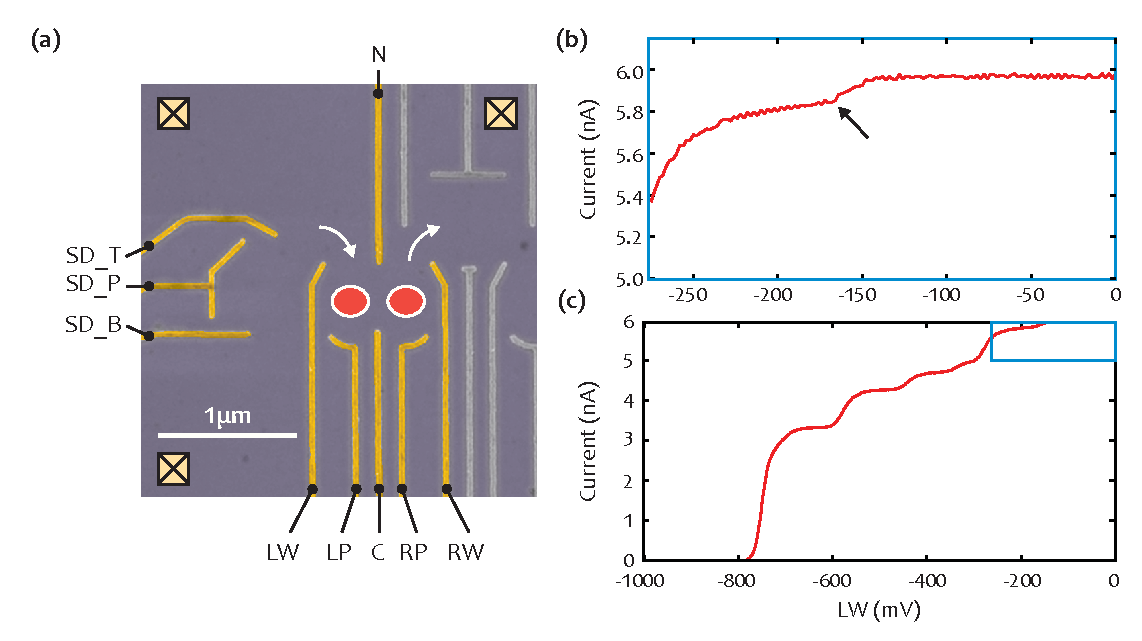
\includegraphics[width=0.9\linewidth]{Device}
  \caption[SEM image of a double quantum dot on GaAs]
  {\label{fig:dd_design}(a) False color SEM of a double quantum dot design on GaAs. Surface gates (highlighted in gold) are
  12nm TiAu onto which negative voltages are applied to deplete the 2DEG 101nm underneath. The locations of the quantum dots are
  highlighted with red circles and the ohmic contacts to the 2DEG in yellow boxes. Descriptions of the gates are given in the
  main text. The width of the double quantum dot at the surface is 970nm. (b) The left wall passing through depletion while
  pinching off with the nose (set to -800mV), at the location marked with the arrow. All other gates are at zero. (c)
  A full pinch-off curve of the left wall against the nose. As the undepleted region of the 2DEG shrinks towards the Fermi
  wavelength, a 1D channel is formed, causing the appearance of quantized conductance plateaus.}
\end{figure}

The design of gate structures that can confine electrons into quantum dots is an area of continued and fruitful research (see for
example Section~\ref{sec:5dot} of this thesis), however a common and well-tested pattern for a double quantum dot is shown in Fig.~\ref{fig:dd_design} (a).
Gates are designed to correspond to the various parameters we described in Section~\ref{sec:qd}; with the gates labelled LW (left wall)
and RW (right wall) controlling the tunnel rates from the reservoirs to the dots, the gate labelled C (centre) controlling the tunnel coupling
$t_c$, and LP (left plunger) and RP (right plunger) controlling the chemical potential of the left dot ($\mu_1$) and right dot ($\mu_2$) respectively.
The N (nose) gate acts as a global control, and a charge sensor (discussed in Section~\ref{sec:readout}) which in this case is a third quantum dot formed
against the left wall is placed to the left of the device. The location of ohmic contacts is marked by crosses and allows us to measure current both
through the device and through the sensor.

The left wall of the quantum dot passing through depletion is shown in Fig.~\ref{fig:dd_design} (b) at the
location marked by the arrow. A full pinch-off trace for the gate is given in Fig.~\ref{fig:dd_design} (c), showing the appearance of quantized
conductance steps as the undepleted region of 2DEG shrinks to towards the Fermi wavelength. These steps appear in units of the spin-degenerate conductance quantum,
$R = 2 n e^2/h$ for integer $n$, the physics of which we discuss in more detail in Section~\ref{sec:char}. Several gates on the device
are wired up to allow the application of radio frequency tones or fast pulses to drive qubit rotations.
Further details of how this is accomplished are given in~\ref{sec:setup}.

\subsection{Qubits from Quantum Dots}
As we discussed at the beginning of this section, one of the challenges of quantum computing is finding physical systems
suitable to be used as qubits. They must be expressible as a two-level system, isolated enough that the quantum state is
preserved during operations, and easily read-out and controlled. The last of these requirements is effectively the
same as finding a system whose Hamiltonian ($H$) can express the operations that we defined in Section~\ref{sec:qc}. We use
Schrödinger's equation to describe this evolution:
\begin{equation}
  i \hbar \diff{\ket{\psi(t)}}{t} = H \ket{\psi(t)}
\end{equation}
For this reason, Hamiltonians describing two level systems used in quantum computers are often explicitly defined in terms of
the Pauli matrices we defined in equation~\ref{eq:pauli}. For example, a model qubit Hamiltonian may be given by:
\begin{equation}
  H = A \sigma_X + B \sigma_Z = \svec{B&A\\A&-B}
\end{equation}
which describes rotations around an axis of the Bloch sphere at angle $\theta = \tan^{-1}\left(\tfrac{A}{B}\right)$ and with a rate
$\omega_r = \tfrac{\sqrt{A^2 + B^2}}{\hbar}$. By varying the values of $A$ and $B$, we are able to construct arbitrary
rotations around the Bloch sphere. Alternatively, the application of photons at the frequency
$\omega_e = 2\sqrt{A^2 + B^2}$ is able to drive transitions between the eigenstates of this Hamiltonian.

\subsubsection{The Charge Qubit}
Perhaps the simplest form of qubit we can form with a double quantum dot system is a charge qubit. Here we define
the logical subspace of the qubit as spanned by two charge states, typically the $(0, 1)$ and $(1, 0)$ charge states,
with the basis $\ket{0} = (0, 1)$ and $\ket{1} = (1, 0)$. The single qubit Hamiltonian is given by:
\begin{equation}
  H_{\textrm{charge}} = \frac{1}{2}\varepsilon\sigma_Z + t_c\sigma_X
\end{equation}
which is represented by the energy level diagram in Fig.~\ref{fig:dqdenergy}. The qubit is typically operated by the application
of microwave pulses with frequency $\Omega = \sqrt{\varepsilon^2 + (2 t_c)^2}$ in order to drive transitions between the ground and
excited charge configurations, and the state is read out via a proximal charge sensor (discussed in Section~\ref{sec:readout}).

Such a qubit, while conceptually simple is highly sensitive to charge noise in the semiconductor, such that the qubit lifetime $T_1$ and
coherence times $T_2$ are both on the order of \SI{10}{\nano\second}~\cite{PhysRevLett.105.246804}. As such, the usefulness of such a qubit
is limited.

\subsubsection{The Loss-DiVincenzo (Single Spin) Qubit}
The next idea for the implementation of a qubit would be to use the spin of a single electron as our two-level subsystem. In
many ways, spin is an ideal phenomenon to use. It is naturally two levels, and as such has no leakage states that our qubit
may accidentally end up in and can easily be implemented using quantum dots~\cite{PhysRevA.57.120}. We can represent the $\ket{0}$ and $\ket{1}$ states
by the spin down and up states ($\ket{\downarrow}$ and $\ket{\uparrow}$) respectively. The splitting between the two states
is controlled by the application of an external magnetic field that causes a Zeeman splitting $\Delta E_Z = g^* \mu_B B$. Since the
spin of an electron does not couple to electric fields (to first order), this gives the single-spin qubit some resistance to
charge noise in the semiconductor. Of course, this also makes the control of the qubit more challenging, as we now require
an oscillating magnetic field to control the qubit. As such, the Hamiltonian, and the control of such a qubit will vary depending on
how we achieve our qubit control. There are four common methods described in the literature for controlling
single spin qubits:
\begin{enumerate}
  \item \textbf{Electron Spin Resonance (ESR)} An alternating magnetic field is generated by an alternating current run through a proximal ESR gate,
        with a frequency matching the Zeeman splitting~\cite{nnano.2014.216}. However, this method of driving rotations is relatively
        slow (on the order of a few \si{\micro\second}) and requires large microwave powers.
  \item \textbf{Electron-Dipole Induced Spin Resonance (EDSR)} In materials with strong spin-orbit interaction, we can
        use the effective magnetic field felt by an electron in motion in a confining potential. Such techniques utilize an AC electric
        field to "wobble" the electron wave function to drive rotations within a single dot~\cite{Nowack1430,nature11559}. This technique
        achieves spin rotations in $\approx \SI{100}{\nano\second}$ in GaAs, down to $\approx \SI{10}{\nano\second}$ in InAs with a stronger spin-orbit coupling.
  \item \textbf{Electrically-Driven ESR in a Slanted Magnetic Field} In materials without strong spin-orbit interaction,
        we can generate an effective oscillating magnetic field by generating a strong magnetic field gradient across a quantum dot with the use of a micromagnet.
        Again, the "wobble" of the electron wave function drives rotations of single spins in a single dot~\cite{PhysRevLett.107.146801}
        or between two quantum dots~\cite{2019arXiv190500346C}. This technique allows rotations on the order of $\approx \SI{10}{\nano\second}$.
  \item \textbf{Electrically-Driven ESR in the Exchange Field of an Auxilliary Spin} The use of an auxiliary spin against
        which we can drive rotations via the exchange interaction again  allows electric field control of spin with sub-nanosecond operation times~\cite{PhysRevB.90.235311}.
        In many ways, this method of control is similar to that of the singlet-triplet qubit, described below, with the exception that we still use a single
        spin as our logical subspace. However, such control has not yet been realized.
\end{enumerate}

As mentioned above, although we have first-order insensitivity to electric fields, the slow speed of ESR leads us to
reintroduce an electric field coupling, either via intrinsic material properties via the spin-orbit interaction, or through
the creation of gradient magnetic fields, to allow for fast control of these qubits. Even then the effect of charge noise
is far lower than for a charge qubit, with coherence times of hundreds of microseconds possible. Additional sources
of noise originate from the coupling between electron spins and the nuclear spins of nearby spinful nuclei. This
effect is termed the Hyperfine interaction, and leads to a fluctuating field, termed the Overhauser field, with magnitude:
\begin{equation}
  B_{\textrm{nuc}} = \frac{1}{g^* \mu_B} \sum^N_n A_nI_n
\end{equation}
where $I_n$ is the nuclear spin operator for the n-th nucleus, and $A_k$ is the coupling strength of that nucleus with the
electron spin. We can treat the Overhauser field as a classical random variable with a Gaussian distribution around zero net
polarization. The RMS fluctuation of $B_{\textrm{nuc}}$ is $\sigma_B = \tfrac{\SI{4.0}{\tesla}}{\sqrt{N}}$ where N is the number of
nuclei that an electron in a quantum dot overlaps\cite{PhysRevB.76.035315}. For GaAs this is typically on the order of $N \approx 10^6$.
This effect is minimized by the use of isotopically purified silicon~\cite{itoh_watanabe_2014}, which contains a
reduced density of spinful nuclei.

\subsubsection{The Singlet-Triplet Qubit}
The use of a single spin, while having a convenient mapping to qubit states, requires either the application of an AC magnetic field
or an AC electric field coupled with some form of gradient magnetic field or spin-orbit interaction. By creating ensembles of
spin, we can trade off a more straightforward system for one with more flexible control or greater immunity to certain types of noise.
The use of two electrons across two quantum dots allows us to use purely pulsed DC control to achieve full control
over the qubit. For this type of qubit, we define our computational subspace as spin states of two coupled electrons, choosing
$\ket{S}$ and $\ket{T_0}$ as our $\ket{0}$ and $\ket{1}$ state respectively, with a Hamiltonian described by:
\begin{equation}
  H = J(\varepsilon)\sigma_Z + g^* \mu_B \Delta B_X \sigma_X
\end{equation}
The fixed gradient field $\Delta B_X$ is achieved either through the use of a micromagnet or via the polarization of the nuclear
field~\cite{PhysRevLett.105.216803}, where $\Delta B_X$ describes the difference in the field seen by an electron in the left and
right quantum dots. An external magnetic field is required to break the degeneracy of the three triplet states, such that
we only operate in the $S-T_0$ states. Any leakage into the $T_-$ or $T_+$ states is undesirable.

\begin{figure}
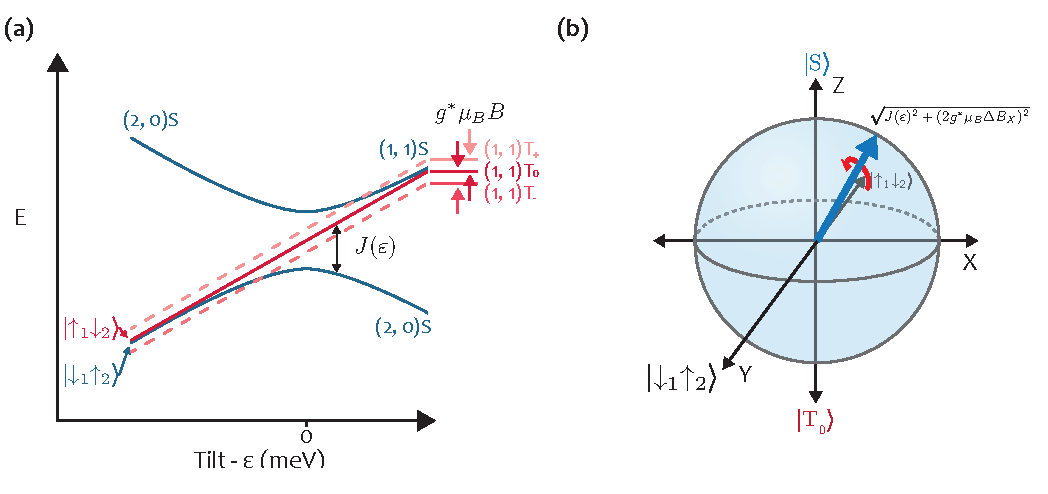
\includegraphics[width=0.9\linewidth]{st0}
\caption[Energy levels and eigenstates of a Singlet-Triplet qubit]
{\label{fig:st0}(a) The energy levels of a Singlet-Triplet Qubit. The three triplet states are split by the application of a
uniform magnetic field $B$. At a large negative detuning, i.e. $J(\epsilon) \approx 0$, the gradient magnetic field $\Delta B_X$ leads to a
change in basis, such that the energy eigenstates are described by $\ket{\uparrow_1\downarrow_2}$ and $\ket{\downarrow_1\uparrow_2}$,
where here we've arbitrarily chosen $\Delta B_X > 0$.
(b) Bloch sphere representation of a single Singlet-Triplet qubit. Qubit rotation proceeds around the axis in blue,
which may be varied by pulsing tilt ($\varepsilon$). The gradient field $\Delta B_X$ is usually constant, set either
by nuclear fields or a fixed micromagnet.}
\end{figure}

The energy levels of such a qubit are shown in Fig.~\ref{fig:st0} (a). The qubit may be easily initialized in the $(2, 0)S$ state via
the exchange of electrons with the reservoirs, as the $(2, 0)T$ states are energetically inaccessible for small tilt and offset [as we
saw in~\ref{fig:dqdenergy} (d)]. In general, $S-T_0$ qubit rotations are driven around an axis set by the relative magnitudes
of $J$ and $\Delta B_X$, as is shown in Fig.~\ref{fig:st0} (b), however, by pulsing tilt, we are able to drive rotations around the Z axis
when $J(\varepsilon) \gg g^* \mu_B \Delta B_X$, or around the X-axis when $g^* \mu_B \Delta B_X \gg J(\varepsilon)$. An equivalent way of
expressing this is to speak in terms of energy eigenstates: for large $J(\varepsilon)$, the two eigenstates of the qubit are $\ket{S}$ and
$\ket{T_0}$, while for $J(\varepsilon) \approx 0$, the energy eigenstates of the qubit are set by the gradient field $\Delta B_X$, with
the ground state given by spins anti-aligned with the gradient magnetic field (since $g^* < 0$ in GaAs), and the excited state by spins aligned with
the gradient magnetic field. Lifetimes for singlet-triplet qubits are primarily limited by coupling to nuclear spins via the hyperfine
interaction~\cite{nnano.2016.170}, which causes fluctuations in the coefficient of $\sigma_X$, as well as charge noise that is ever present
in semiconductor-based systems~\cite{PhysRevLett.110.146804}. Despite this, coherence times have been extended in GaAs spin qubits to
over \SI{200}{\micro\second} via the use of dynamical decoupling sequences~\cite{nphys1856}.

It is also worth mentioning that there is active research in optimizing the control schemes for singlet-triplet qubits, again with
the intention of gaining resistance to certain forms of noise. For example, recent results suggest that variation of $J(\varepsilon)$ by modulation of
tunnel coupling $t_C$, leading to symmetric pulses on the left and right quantum dot~\cite{PhysRevB.73.205302,PhysRevB.97.155402,PhysRevLett.116.116801,PhysRevLett.118.216802},
or the use of magnetic field gradient estimation and active control~\cite{ncomms6156,s41534-016-0003-1} may lead to higher
fidelity control and reduced dephasing. Further reduction in charge noise is expected with
improved materials growth, which is expected to further extend qubit coherence times~\cite{PhysRevApplied.9.034008}.

\subsubsection{The Exchange-Only Qubit}

\begin{figure}
  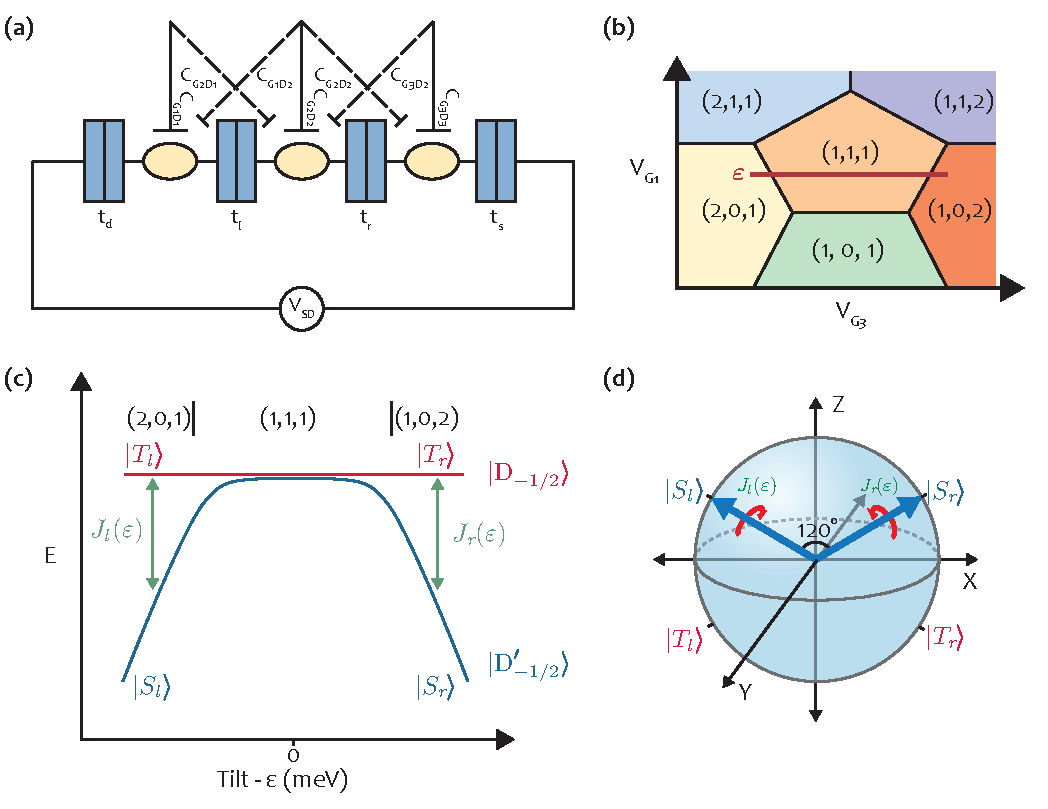
\includegraphics[width=0.95\linewidth]{eo}
  \caption[Energy levels and eigenstates of an Exchange-Only qubit]
  {\label{fig:eo}(a) Schematic of a triple quantum dot, with tunable tunnel couplings between the left and centre quantum dots, and the
  right and centre quantum dots. (b) Charge stability diagram for a triple quantum dot when sweeping the $V_{G1}$ and $V_{G3}$ around the
  $(1,1,1)$ charge configuration. The tilt axis is marked in red and sweeps from the $(2,0,1) \rightarrow (1,1,1) \rightarrow (1,0,2)$
  charge configurations. (c) Energy levels of the exchange-only qubit. Quadruplet states or excited doublet states are not shown. The Exchange energies
  between the left (right) and centre dots are swept as a function of tilt. The energy eigenstates change between $\ket{S/T_l}$ and $ket{S/T_r}$
  at the extremes of tilt. (d) Bloch state representation of the exchange-only qubit. The exchange interaction drives rotation around two
  axes of the Bloch sphere separated by \SI{120}{\degree}.}
\end{figure}

While the singlet-triplet qubit described in the above section allows us to control our qubits with only fast pulses, they still require
a spatially varying magnetic field for full two-axis control. The use of three electrons distributed through three quantum dots allows
for fully electrical control of a spin qubit using only exchange interactions between the left and centre, and right and centre quantum
dots~\cite{10.1038-35042541}, as shown in Fig~\ref{fig:eo} (a) and (b). In this case, the system has a total of eight possible spin states. These
are one set of quadruplet states with total spin $S^2 = 3/2$ and spin projections $S_Z = \{-3/2, -1/2, +1/2, +3/2\}$, and two sets of doublet
states corresponding to a singlet or triplet in the left (right) dot, and a third spin on the right (left) dot. The choice of placing the singlet/triplet
state on the left or right dot is set by the tilt, with the energy eigenstates of the system given by the singlet/triplet state on the left for $\varepsilon \ll 0$,
and on the right for $\varepsilon \gg 0$. We can, therefore, write out the four doublet states as
\footnote{The full set of eigenstates at different values of $J_l, J_r, \varepsilon$ can be found in~\cite{PhysRevB.82.075403}}:
\begin{equation}
\begin{split}
  \ket{\textrm{D}_{-1/2}}        &= \ket{\uparrow T_R}   (\textrm{for }\varepsilon \gg 0) = \ket{T_L\uparrow}   (\textrm{for }\varepsilon \ll 0)\\
  \ket{\textrm{D}_{+1/2}}        &= \ket{\downarrow T_R} (\textrm{for }\varepsilon \gg 0) = \ket{T_L\downarrow} (\textrm{for }\varepsilon \ll 0)\\
  \ket{\textrm{D}^\prime_{-1/2}} &= \ket{\uparrow S_R}   (\textrm{for }\varepsilon \gg 0) = \ket{S_L\uparrow}   (\textrm{for }\varepsilon \ll 0)\\
  \ket{\textrm{D}^\prime_{+1/2}} &= \ket{\downarrow S_R} (\textrm{for }\varepsilon \gg 0) = \ket{S_L\downarrow} (\textrm{for }\varepsilon \ll 0)\\
\end{split}
\end{equation}

In order to break the degeneracy of the third spin, a global magnetic field is applied, such that we are left with our computational basis states, which
I arbitrarily choose to be the $-1/2$ states here:
\begin{alignat}{2}
  \ket{0} &=& \ket{\textrm{D}^\prime_{-1/2}} &= \ket{S_{l,r}} \\
  \ket{1} &=& \ket{\textrm{D}_{-1/2}} &= \ket{T_{l,r}}
\end{alignat}

Focussing on this subspace, the energy level diagram of the exchange-only qubit is given in Fig.~\ref{fig:eo} (c). We are able to change the exchange
energy between the left (right) and center dots by sweeping tilt ($\varepsilon$). We can largely ignore leakage states as the set of four quadruplet
states have different principal spin, and the two remaining doublet states are rendered inaccessible by the applied Zeeman field. The exchange-only
qubit was first experimentally realized in~\cite{PhysRevB.82.075403}. In GaAs systems, rotations at rates of up to \SI{47.4}{\giga\hertz} have been measured,
with a lower bound of $T_2 = \SI{100}{\nano\second}$, limited by nuclear spins in GaAs~\cite{nnano.2013.168}.

The fast rotation rate also leads to increased sensitivity to exchange (charge) noise, however improved schemes building
on the ideas of the exchange-only qubit~\cite{Russ_2017}, such as the Resonant Exchange Qubit~\cite{PhysRevLett.111.050501},
the Always-On Exchange-Only (AEON) qubit~\cite{PhysRevB.93.121410} or the Quadrupolar Exchange-Only Qubit~\cite{PhysRevLett.121.177701,Kornich_2018},
which trade off the number of electrons or requirements to continuously drive the system for insensitivity to certain forms of noise.
Additional work with double quantum dots with higher electron occupancies and hence higher principal spin quantum numbers are also
predicted to have desirable noise rejection, while still allowing fully electrical control, such as the hybrid
spin/charge-qubit~\cite{PhysRevLett.108.140503}, which has recently shown an ensemble dephasing time
of $T_2^* = \SI{8.1}{\nano\second}$ with rotation rate $f_{\textrm{rabi}} = \SI{2.43}{\giga\hertz}$ in
GaAs~\cite{PhysRevLett.116.086801} or $T_2^* = \SI{2}{\nano\second}$ with rotation rate $f_{\textrm{rabi}} = \SI{5.2}{\giga\hertz}$ in
Si/SiGe~\cite{nature13407}, which is presently limited by charge noise~\cite{s41534-017-0034-2}.

\clearpage

\subsection{Majorana Zero Modes}
\label{sec:majo}


\subsection{Characterizing 2DEGs}
\label{sec:char}
\subsubsection{The Quantum Hall Effect}
\subsubsection{Spin Orbit Interaction}

\section{Architecture of a Quantum Computer}
\label{sec:arch}
  \subsection{Control Plane}
  \subsection{Readout}
  \label{sec:readout}
% \chapter{Architecture of a Quantum Computer}
\label{sec:arch}
Although the challenges of building a fault-tolerant qubit have by no means been met, the field is rapidly reaching the point where
it is possible to start running algorithms on quantum computers. While algorithms such as Shor's algorithm for prime factorization
would require $2N + 3$ logical qubits with an arbitrarily long lifetime~\cite{Beauregard:2003,6657074}, other algorithms may
be able to achieve a quantum speedup with a limited number of noisy qubits. Algorithms and systems operating in this regime are
said to be in the Noisy Intermediate-Scale Quantum (NISQ) regime~\cite{Preskill2018quantumcomputingin}, a term coined by John Preskill
in 2018 to distinguish between a full-scale quantum computer, with a large number of error corrected qubits, and one that we may realize
in the coming decade, containing as few 10s of noisy, imperfect qubits. In the near term, the race is on to achieve \textbf{quantum supremacy},
a calculation on a quantum computer whose simulation on a classical computer is intractable. The expectation is that this milestone will
be beaten in the coming years, with a system of approximately 50 noisy qubits~\cite{s41567-018-0124-x}. Based on the current state of the field
this will likely occur using superconducting transmon-like qubits solving a model problem such as Boson sampling~\cite{Aaronson:2011}. While such a
result would certainly be groundbreaking, the more interesting result would be a demonstration of \textbf{quantum advantage}, an algorithm whose simulation on a
classical computer is intractable, but one which also solves a useful problem. While Boson sampling certainly seems to be a classically hard problem,
the solution it provides does not seem to be one that has many practical implications. In the near term, our best bet for achieving a useful result
seems to be using the Variational Quantum Eigensolver algorithm \cite{ncomms5213}, which, as we alluded to in the introduction of Chapter~\ref{sec:quest}, would allow us
to model molecules that we could not on a classical computer, with a small number (100s) of imperfect qubits~\cite{PhysRevA.92.042303}.
To date, several experimental realizations of this algorithm have been published~\cite{nature23879,PhysRevX.8.011021,10.1038/s41586-019-1040-7},
although none have yet simulated a molecule that is classically intractable~\cite{Reiher7555}.

\section{Designing an Architecture}
Given the rapid progression of the field, the questions surrounding architecting a quantum computer have been gaining increasing attention,
particularly as the number of qubits grows beyond the limits that we might control with a ad-hoc architecture that a single graduate student might construct.
The challenge for experimentalists continues to come down to building scaleable building blocks, which balance the need for experimental
flexibility surrounding qubits whose designs and control requirements remain in flux, but whose footprint does not explode for larger numbers
of physical qubits. Thankfully, at least within the realm of solid-state qubits (that is superconductor and semiconductor based qubits),
there is substantial overlap in the requirements for control and readout of qubits, that allows us to design architectures for hypothetical
quantum machines. Let's therefore enumerate a number of requirements for a control and readout architecture controlling a solid-state qubit:
\begin{itemize}
  \item \textbf{Cryogenic operation}: Solid-state qubits must be operated in cryogenic environments, stemming from the requirement that the thermal energy should be well below the level spacing of energy levels in the qubit, as well as the need for superconducting elements in some designs. Any control and readout architecture must, therefore, be low power, and avoid carrying thermal energy or noise down to the qubit device.
  \item \textbf{Control fidelity}: In order to reach the fault-tolerance threshold, fidelities of individual qubits must exceed $99\%$, and should ideally be well above the $(1 - 10^{-5})$ level to avoid prohibitive error correction requirements~\cite{6657074}. Depending on the rotation rate and decoherence rates of individual qubits, control lines must have bandwidths of several 10's of \si{\giga\hertz}, along with high density, low crosstalk and low noise.
  \item \textbf{Readout fidelity}: Readout of qubits brings unique challenges, requiring low probe powers in order to avoid disturbing the state while it is being measured, and limited measurement time due to decoherence. In addition, QEC in general requires the continued measurement of ancilla qubits while nearby qubits are operational, leading to stringent crosstalk requirements. In order to obtain a sufficient signal-to-noise ratio, cryogenic amplification is generally required, which in turn limits and scaleable design to one, or a few, readout lines. As such, some form of multiplexing, either frequency-domain or time-domain, is necessary for readout.
  \item \textbf{Space}: This requirement is particularly difficult to accomplish as it occurs over three orders of magnitude over the scale of the chip, the cryostat and at room temperature. Each of these are discussed in detail below, but we state the problem briefly here. On a chip scale, dense control lines must be fit into an area set by the distance over which we can achieve coupling between qubits, setting micron-scale limits on on-chip structures. On a cryostat level, the need to operate at \si{\milli\kelvin} in a cryostat places centimeter-scale limits on cryogenic components. Finally at room temperature, phase matching of control pulses and the need for active feedback places limits on the size of the instrumentation used to control individual qubits.
\end{itemize}

\afterpage{
  \clearpage
  \thispagestyle{empty}
  \begin{landscape}
  \begin{table}
    \centering
    \def\arraystretch{1.5}
    \begin{tabular}{|l|l|l|l|l|l|l|}
    \hline
    \multicolumn{3}{|l|}{} & \shortstack{CryoCMOS Architecture\\(Section~\ref{sec:gooseberry})} & \shortstack{Prime-Lines Architecture\\(Section~\ref{sec:primelines})} & \shortstack{Frequency\\Multiplexed~\cite{doi:10.1063/1.4868107}} & \multicolumn{1}{|c|}{Na\"ive} \\
    \hline
    \multirow{5}{*}{Room Temp}  & \multirow{2}{*}{Power} & $P_{C,RT}$    & $\SI{100}{\watt}$ & $M\times\SI{1000}{\watt}$ &$N\times\SI{1000}{\watt}$ &$N\times\SI{1000}{\watt}$\\\cline{3-7}
                                &                        & $P_{R,RT}$    & $\SI{100}{\watt}$ & $N\times\SI{100}{\watt}$ & $N\times\SI{100}{\watt}$ & $N\times\SI{100}{\watt}$\\\cline{2-7}
                                & \multirow{3}{*}{Lines} & $N_{DC,C,RT}$ & 3                         & $N$                      & $N$ & $N$                 \\\cline{3-7}
                                &                        & $N_{RF,C,RT}$ & 3                         & M                        & $N$ & $N$                 \\\cline{3-7}
                                &                        & $N_{RF,R,RT}$ & 2                         & 2                        & 2   & $N$                 \\\hline
    \multirow{5}{*}{4K} & \multirow{2}{*}{Power} & $P_{C,4K}$    & $\SI{1}{\watt}$        &$\SI{1}{\watt}$        & $N\times\SI{4}{\micro\watt}$   & $N\times\SI{4}{\micro\watt}$                   \\\cline{3-7}
                        &                        & $P_{R,4K}$    & $\SI{50}{\milli\watt}$ &$\SI{50}{\milli\watt}$ & $\SI{50}{\milli\watt}$ & $N\times\SI{50}{\milli\watt}$\\\cline{2-7}
                        & \multirow{3}{*}{Lines} & $N_{DC,C,4K}$ & 3                         & $N$                      & $N$ & $N$                 \\\cline{3-7}
                        &                        & $N_{RF,C,4K}$ & 3                         & $M$                      & $N$ & $N$                 \\\cline{3-7}
                        &                        & $N_{RF,R,4K}$ & 2                         & 2                        & 2   & $N$                 \\\hline
    \multirow{4}{*}{mK} & \multirow{2}{*}{Power} & $P_{C,mK}$ & $N\times\SI{0.01}{\micro\watt}$ & $ N\times\SI{1}{\micro\watt}$ & $N\times\SI{1}{\micro\watt}$   & $N\times\SI{1}{\micro\watt}$                   \\\cline{3-7}
                        &                        & $P_{R,mK}$ & \SI{40}{\nano\watt}     & \SI{40}{\nano\watt}           &\SI{40}{\nano\watt}   & $N\times\SI{40}{\nano\watt}$ \\\cline{2-7}
                        & \multirow{2}{*}{Lines} & $N_{C,mK}$ & $N$                     & $N$                           & $N$ & $N$                 \\\cline{3-7}
                        &                        & $N_{R,mK}$ & $N$                     & $N$                           & $N$ & $N$                 \\\hline
    \end{tabular}
    \caption[Approximate power and wiring requirements for a QC]{Order of magnitude power $P$ and wiring $N$ requirements for the CryoCMOS architecture, the Prime-Lines architecture, frequency multiplexed readout and a Na\"ive architecture. The number of lines is split between high-bandwidth coaxial lines (RF) and low-bandwidth (DC) lines. In each case, we trade off the complexity in the setup to reduce the wiring required down the fridge. The power consumption and number of lines is given in terms of the number of qubits $N$, and in the case of the Prime-Lines architecture, the number of pulse shapes $M$. Power consumption for control lines is calculated assuming a \SI{10}{\milli\volt} pulse through a \SI{20}{\decibel} attenuator, a \SI{100}{\mega\hertz} repetition rate and assuming approximately \SI{0.5}{\meter} of RG-047 coaxial cable is used between temperature stages. Readout power is calculated assuming a caltech-style HEMP amplifier at the 4K stage, and utilizing rf-reflectometry techniques for readout (see Sec.~\ref{sec:readout}). With a \SI{-90}{\decibel} readout power,
    dissipation is dominated by passive thermal conduction up to $\sim 1000$ simultaneous channels.}
    \label{tab:arch}
  \end{table}
\end{landscape}
}

In general, qubit architectures for solid-state qubits can be classified into two categories (control and readout) at three different temperature stages
(room temperature (RT), four Kelvin (4K) and milli Kelvin (mK)), as shown in Fig.~\ref{fig:genarch}. An
architecture is characterized by the number of RF and DC lines that run between temperature stages $N$, and a power consumption at each stage $P$, divided between the control
and readout block. Two architectures are presented in this this thesis, which trade off complexity and reduced experimental flexibility for reduced wiring and power consumption
at different stages of the cryostat. The CryoCMOS architecture, presented in Sec.~\ref{sec:gooseberry} utilizes a CMOS based switching matrix at that is
bonded directly to the qubit chip in order to minimize the power dissipated in parasitic capacitance. The Prime-Lines architecture, presented in Sec.~\ref{sec:primelines}
utilizes a cryogenic switching matrix near the qubit to minimize the number of high-frequency coaxial lines required to control qubits. Order of magnitude estimates
for the number of control lines and the power consumption for each architecture is given in Table~\ref{tab:arch}, characterized by a number of qubits $N$,
and in the case of the prime-lines architecture, the number of control pulse-shapes $M$, where in general $M \ll N$. The sources of power dissipated for each of these architectures
will be elucidated over the course of the remainder of the section. I will however draw the readers attention to the fact that even for passive, high-bandwidth wiring, there is a
power cost associated with bringing these lines down~\cite{Krinner2019}, a topic I will explore in detail in Sec.~\ref{sec:control}.

\begin{figure}
  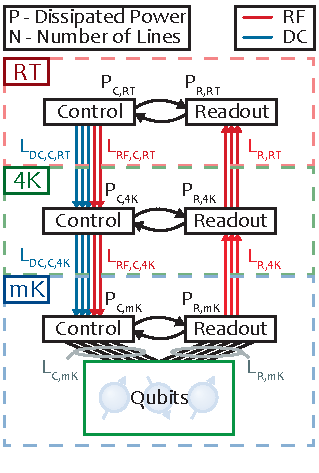
\includegraphics[width=0.5\linewidth]{genarch}
  \caption[Generalized quantum computing architecture]
  {\label{fig:genarch}A generalized qubit architecture, broken into control and readout stages at each temperature stage of a cryostat. The architecture is characterized by number of lines which run between each stage, for example $N_{RF,C,RT}$ for the number of coaxial control lines running from room temperature to the \SI{4}{\kelvin} stage of the cryostat, which will vary depending on the choice of a given architecture. In addition, each stage will dissipate a certain amount of power, for example $P_{R,4K}$ being the power dissipated at \SI{4}{\kelvin} by the readout stage, caused either by active logic, such as an FPGA, amplifiers or off-the-shelf instrumentation, or by passive dissipation, for example due to attenuators.}
\end{figure}

In the remainder of this section, I will quickly review the challenges for control and readout for a large-scale quantum computer, which very much remains
an open question in the field. As we move through the following sections, the sources of many of the numbers in Table~\ref{tab:arch} should become clear
as well as our vision for solving some of these problems. In general, I will progress from the qubit plane up to room temperature control, however this
structure is by no means struct.

\subsection{Control Plane}
\label{sec:control}
A popular refrain for proponents of semiconductor-based qubits is to point to the maturity and flexibilty of modern semiconductor processing as an argument
for the scalability of qubits based on similar processes. While it is undoubtedly true that the miniaturization of transistors has translated into an ability
to fabricate finer devices, the scalability of quantum computers based on such an argument is by no means as clear. The problem, and indeed the main diffrentiator
between a qubit and a transistor, it that while a transistor has the ability to drive other transistors, a qubit has no similar ability. All control of a qubit
must come from outside. This unfortunate fact is captured in Rent's rule, which relates the number of external terminals (or pins) $T$ of an IC, to the number of
internal components (or transistors) $g$:
\begin{equation}
  T = tg^p
  \label{eq:rent}
\end{equation}
where t and p are constants of the system. For an integrated circuit, the value of $p$ generally ranges from 0.5 to 0.8~\cite{5388820}, however for a quantum
circuit, it is reasonably simple to see that this exponent must be 1! Each qubit must be driven by some number $t$ gates, with no qubit able to drive another
qubit without some external control.

The above statement captures the primary difficulty that we will run into when designing qubit chips. While classical ICs can rely on some fan-out to minimize
the number of inputs required, the design of a quantum chip must be able to bring supply high density wiring with high bandwidth and low cross-talk. In addition,
classical CMOS processes usually have only a few layers of high-density interconnect, used only for short-range connections~\cite{5424258}, while qubit
architectures generally require several layers of high-density interconnect over the length of an entire chip~\cite{s41467-017-01905-6}. The question then is
what sets the maximum pitch of a qubit on a chip, as this gives us the density of control lines that must be achieved. Then, given that pitch, how many lines could
we bring in to such a device, given a 1D or a 2D grid of qubits?

The answer to the first question, the pitch of qubit devices, will be set by the length scale over which coupling can be achieved. For spin qubit devices based only
on direct exchange for example, the pitch of qubits will be roughly the size of the qubit itself, as coupling only occurs when electrons can directly tunnel between
neighbouring devices~\cite{PhysRevB.86.085423}. Work presented in this thesis uses elongated many-electron quantum dots to increase this to the micron-scale in
Section~\ref{sec:5dot}, an approach which will likely be applicable majorana devices that use quantum dots as couplers~\cite{PhysRevB.95.235305}. Finally, long
distance coupling of spins via superconducting resonators~\cite{PhysRevB.97.235409} has recently been demonstrated~\cite{2019arXiv190500776B}, enabling coupling
over \si{\milli\meter} length scales.

The next question is how many lines we can bring to a device. In a 1D device geometry, that is for a single line of qubits, the answer is limited only by the
physical size of the chip, and the size of pads (bond pads or bump pads) that we are able to make contact to. For example, a singlet triplet qubit which requires
10 control lines, and pads of pitch $100\times100\si{\micro\meter}$ will require a chip with a \SI{0.01}{\square\milli\meter} area, assuming of course that we are
able to make contact in 3D (i.e. overlapping bonds). In the case that we are only able to make contact in 2D, a chip of size $400\times400\si{\micro\meter}$ at a
minimum is required to break pads out to the edge of a device. The situation is more difficult to evaluate in a 2D array. Firstly, a 2D array is not possible on
a single planar grid, as control lines for inner qubits must be broken out. Therefore a sufficient distance between qubits must be possible to allow control lines
to be brought in from upper layers. To allow fanout of a dense grid leads to a problem very similar to that of routing a BGA package. There will be a relationship
between number of layers, track pitch and via (inter-layer contact) pitch, which will set a hard density limit on qubit devices. Therefore increasing the pitch of
qubit devices via long distance coupling may be necessary when moving to 2D grids. Furthermore, the design of qubit layouts allowing realistic wiring schemes will
continue to be crucial moving forwards~\cite{10.1038/s41534-018-0074-2}. Finally, I point to the potential for multiplexing the control of many qubits onto single
control lines, which may allow the definition of a quantum analog to Rent's rule~\cite{FRANKE20191} (Equation~\ref{eq:rent}). Whether such an architecture is truly
scaleable remains an open question at this time.

While on a single qubit chip, it seems difficult to get around the problem of breaking all control lines out in order to allow qubit control, however, alluding
back to our generalized qubit architecture in Fig.~\ref{fig:genarch}, it should in general be possible to reduce the number of lines running between the 4K stage
and the control plane at mK. To understand why the techniques for doing so, it is useful to separate control pulses into three general forms, microwave excitations,
fast pulses and static confinement. The first two of these require high bandwidth rf wiring, while the latter requires only low bandwidth dc wiring. By the use of
CryoCMOS switches, as detailed in Section~\ref{sec:gooseberry}, it is possible to multiplex a single DC control line to several gates, effectively locking
a voltage onto those gates. Such switches do not dissipate power except when toggled, leading to extremely low power consumption. Similarly, fast pulses may similarly
be generated, again, as detailed in Section~\ref{sec:gooseberry}, minimizing the parasitic capacitance and hence power dissipation, given by $P_\textrm{diss} = CV^2f$
caused by the length of control lines. This leads to the low power consumption of the CryoCMOS architecture in Table~\ref{tab:arch}. The availability of CMOS at low
temperature also gives us a possible solution to the high interconnect density previously discussed, as the pitch of bump-bonding technologies approaches a few \si{\micro\meter}
(with the smallest I am aware of in use at the time of submission being \SI{20}{\micro\meter}~\cite{4550089}). Similarly, the design of low-dissipation and highly integrated
rf-switches as demonstrated in Section~\ref{sec:primelines} allows the routing of a few microwave or pulse lines, which provides a path to further reduction of the footprint
of wiring between stages of the cryostat, as well as a reduction of the signal generation equipment required.

The thermal cost of high bandwidth control must also be considered when designing control systems for quantum computing applications. As qubits must be operated at low
temperature and are highly susceptible to thermal noise, we must design wiring to attenuate the thermal photon population at the qubit plane. Primarily this is achieved
through the use of dissipative attenuation at each stage, where the population of thermal photons at each stage can be calculated as~\cite{Krinner2019}:
\begin{equation}
  n_i(\omega) = \frac{n_{i-1}(\omega)}{A_i} + \frac{A_i - 1}{A_i}\frac{1}{\exp(\hbar\omega/k_BT_i) - 1}
\end{equation}
where $T_i$ is the temperature and $A_i$ is the attenuation on the $i$-th stage of the cryostat. The first term of this equation gives the attenuation of thermal photons
from the previous stage ($n_{i-1}$), while the second term gives the thermal photon flux spectral density generated by the attenuator itself. As such, to reduce thermal photons,
attenuation must be used at the lowest temperature stages of the order of \SI{20}{\decibel}, to achieve $n_\textrm{mK}(\SI{6}{\giga\hertz}) \sim 0.002$ .Therefore,
even without considering the heat load due to the thermal conductivity of coaxial cables, a significant portional of the power for control must be dissipated
in the filtering of thermal photons. For Table~\ref{tab:arch}, this heat load is estimated at \SI{1}{\micro\watt} per coaxial line, comprising primarily of
$CV^2f$ dissipation, assuming a \SI{10}{\milli\volt} pulse through a \SI{20}{\decibel} attenuator, a \SI{100}{\mega\hertz} repetition rate and assuming approximately
\SI{0.5}{\meter} of RG-047 coaxial cable between temperature stages.

Finally we move up to room temperature, where two primary concerns remain, power consumption and latency (or phase matching), both of which place limits on the footprint
of control electronics at room temperature. In particular, as the rotation rate of qubits is increased, finer tolerances for the phase match of control pulses
is required. When utilizing long control lines, such a phase match is difficult to achieve. Furthermore, as the number of qubits is increased, the footprint of
off-the-shelf electronics, which is in general not designed for simultaneous control of a large number of lines, becomes onerous. In Section.~\ref{sec:primelines}
we address some of these concerns using cryogenic hardware for control, which may allow the use of high density cryogenic interconnects~\cite{Tuckerman_2016}, although
the overall advantages of 4K control require further investigation.

\subsection{Readout}
\label{sec:readout}
In addition to control, the high-fidelity readout of a fragile quantum state is a crucial element of a quantum computer, without which improvements
we make to the control of our qubit are negated. Combining fast, high-fidelity readout with scaleable design complicates the requirements even further,
particularly when we consider the most common desings for readout circuits. As before, I will begin the discussion of readout at the qubit chip level,
and discuss scaleability as we go.

\begin{figure}
  \includegraphics[width=\linewidth]{ReadoutFig}
  \caption[Readout of a semiconductor quantum dot]
  {\label{fig:readout}(a) False color SEM of a five-dot device, similar to the one presented in Sec.~\ref{sec:5dot}. Surface gates are labelled, and
  current is shown running through the charge sensor on the left of the device. (b) Charge sensing signal when the left sensor is tuned as a QPC (1d channel).
  Each step corresponds to a change in the charge occupancy of the quantum dot by 1. (c) Multiplexed readout chip with several resonators, used for
  performing rf readout. (d) Response of the charge sensor in current (right axis) and in reflected rf power (left axis) as the QPC is brought through pinchoff.
  (e) Sample of a charge stability diagram taken using rf charge sensing. Each distinctly coloured region represents a unique charge configuration.}
\end{figure}

For the majority of semiconductor qubit designs, readout is performed via sensing of the charge state of a quantum dot, or quantum dot like
structure. For spin qubits, this is performed by spin-to-charge conversion, where the charge state of a quantum dot will depend on the spin states
of its electrons~\cite{nature02693,PhysRevB.98.125404}, and for Majorana fermions this occurs via the fusion of edge modes (see Sec.~\ref{sec:rfmajo}).
Typically readout is performed via a proximal charge sensor, which may be formed by a quantum point contact (1D channel), or a sensing dot. A gate pattern
with a sensing dot on the left and right is shown in Fig.~\ref{fig:readout} (a). The conductance of the QPC or sensing dot will depend sensitively
on the charge state of the proximal double quantum dot. This is shown in Fig.~\ref{fig:readout} (b), where steps in the conductance of the QPC correspond to
charges moving on and off the nearby quantum dot. The measurement of this conductance can either be done via a dc lockin measurement or via
rf-reflectometry~\cite{Reilly:2007ig}. The dc measurement is limited by the RC-time constant of the wiring in the fridge, which due to the parasitic
capacitance, filtering and high resistance of the sensor will in general limit bandwidth to a few kilohertz, far greater than the T1 times for spin qubits.
RF measurement is performed by embedding the QPC in a resonator, where the quality factor of the resonator is set by the resistance of the charge sensor.
The derivation of the matching condition is not given here, but I point the interested reader towards~\cite{crootthesis}, where a complete derivation is given.
Of course this immediately points towards the possibility of frequency multiplexing~\cite{doi:10.1063/1.4868107}, allowing the readout of multiple
resonators simultaneously, although the requirement for a proximal charge sensor means such an architecture is unsuitable for 2-D architectures. For larger
arrays of charge sensors, the presence of noise generated by the charge sensor can additionally become significant~\cite{PhysRevB.78.035324}, creating
an additional source of dephasing for proximal qubits which we may not wish to disturb.

\begin{figure}
  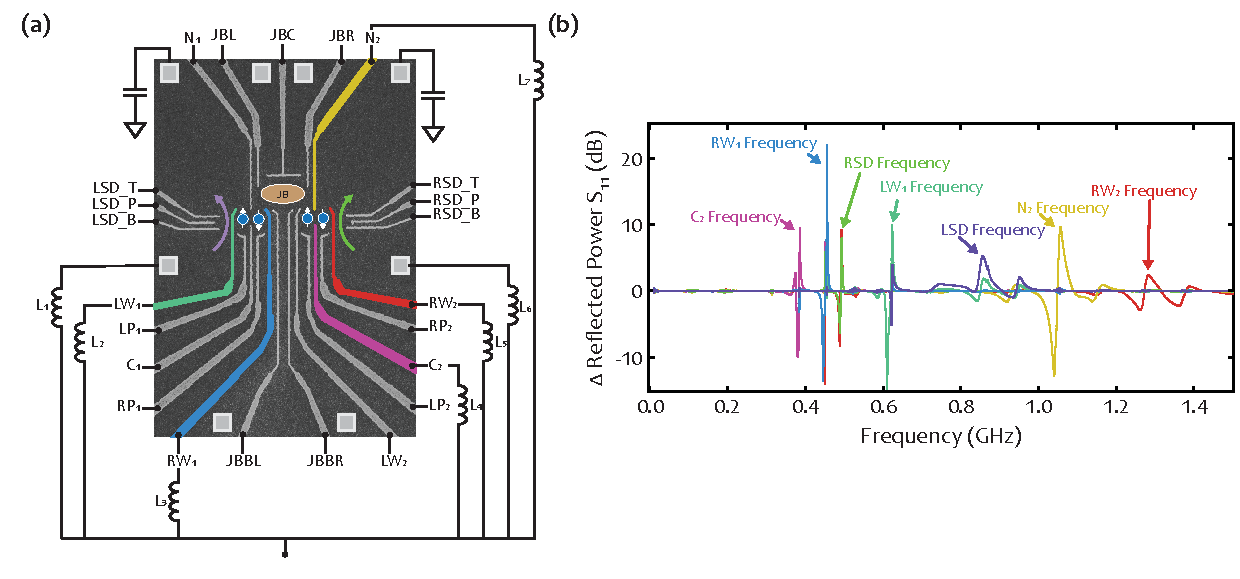
\includegraphics[width=\linewidth]{multifreq}
  \caption[Frequency multiplexed readout of a five-dot device]
  {\label{fig:multifreq}(a) False color SEM of a Five Dot device, identical to the one used in Sec.~\ref{sec:5dot}. A number of resonators are bonded to several gates
  including both charge sensors and dispersive gate sensors. (b) The frequency response of the multiplex chip when the voltage on each gate is changed. Distinct frequencies
  are observed for each gate on the sample.}
\end{figure}

An alternative to using a proximal charge sensor is to use the confining gates themselves as sensors~\cite{PhysRevLett.110.046805}, wherein the quantum capacitance
of the system is measured. The polarizability of a quantum dot is given by:
\begin{equation}
  C_Q = - \diffp[2]{E}{{V_{g}}} = -(\alpha \varepsilon)^2 \diffp[2]{E}{\varepsilon}
\end{equation}
where $\alpha$ is the lever arm and $\varepsilon$ is the tilt, as shown in Fig.~\ref{fig:dqd} and defined in Sec.~\ref{sec:qd}. As we can see from the above equation
the quantum capacitance is proportional to the band curvature, which allows us not only to detect charge transitions but also the spin state (since the triplet state has no
curvature at 0 tilt), and hybridization. The latter effect may be used to detect the parity state of a Majorana zero mode coupled to a proximal
quantum dot~\cite{PhysRevB.95.235305}. As with readout via a charge sensor, by embedding a gate in a resonant circuit, we are able to quickly sense changes
in capacitance, with a sensitivity that is sufficient to perform single shot readout of spin states~\cite{fernando1,Nnano_dzurak}. A frequency multiplexed device
with 7 resonators is shown in Fig.~\ref{fig:multifreq}, combining both dispersive and charge-sensing modes of readout.

The potential for frequency multiplexing also allows us to imagine integrated methods of readout. While the idea of multi-channel qubit readout is certainly
not new, the design of equipment that are able to handle large numbers of channels simultaneously is as yet an open problem. In particular, once multiple
channels are multiplexed onto a single rf pair, the total power that must be transmitted for $n$ channels is:
\begin{equation}
  P_\sum(n) = P_0 + 10 \log_{10}(n)
\end{equation}
At the device level, this increases the isolation necessary between channels, as it is desirable to be able to select qubits to measure selectively. In addition,
crosstalk may drive rotations of neighbouring qubits, reducing the fidelity of control, which is particularly problematic for error correction schemes
where proximal ancilla qubits must be constantly read and corrected.

At this point, it is also worth covering noise in the readout circuit, as noise in the system is the limiting factor in readout time. Unfortunately, as alluded
to in earlier sections, the fragile nature of the quantum state requires us to use low probe powers in order to ensure our readout does not destroy the quantum
state. In quantum dots, we can generally place limits on the power of our probe signal $P_\textrm{probe}$ using similar thermal arguments to those used when discussing
bias, that is the power of the signal should be much less than the relevant energy scales of the system: $P_\textrm{probe} \ll \Delta E$. In the case of circuit-QED,
the requirements are even more strict, where operation in the single photon limit is necessary:
\begin{equation}
  P_\textrm{probe} \sim \frac{\hbar \omega^2}{2} \frac{Q_c}{Q_l^2}
\end{equation}
where $Q_c$ is the coupling-$Q$ and $Q_l$ is the loaded-$Q$ of the resonator. Unfortunately any quantum system will, at the very minimum, generate thermal noise and
vacuum fluctuations. The thermal noise power spectral density, that is the noise power per unit bandwidth, for a system is given
by~\cite{RevModPhys.82.1155}\footnote{Note that this form of noise power spectral density is given by a quantum theory of noise. In the limit
of large temperature ($\hbar\omega \ll k_BT$), using the approximation $\coth (x) \approx 1/x$ for small x, we recover the classical formula for noise power
spectral density: $S(\omega) = k_B T$.}:
\begin{equation}
  S(\omega) = \frac{\hbar \omega}{2}\coth\left(\frac{\hbar\omega}{2k_BT}\right)
\end{equation}
from which we can define an effective noise temperature of the system:
\begin{equation}
  T_\textrm{eff} = \frac{S(\omega)}{k_B}
\end{equation}
We can therefore define the maximum signal-to-noise ratio of a system, that is the signal-to-noise of an ideal receiver at the output of our qubit, for a measurement
bandwidth of \SI{1}{\hertz}:
\begin{equation}
  \textrm{SNR}_\textrm{max} = \frac{P_\textrm{probe}}{S(\omega)}
\end{equation}
In order to read a small signal, since any physical readout hardware will have a limited dynamic range and will itself add noise, additional amplification is necessary.
We must therefore account for the noise added by any given amplifier, with the total effective system temperature:
\begin{equation}
  T_\textrm{sys} = T_{0} + \frac{T_{1}}{G_1} + \frac{T_{2}}{G_1G_2} + \ldots \frac{T_{n}}{G_1G_2 \ldots G_{n}}
\end{equation}
where $T_{0}$ is the noise temperature at the output of the qubit, and will include $T_\textrm{eff}$, the thermal noise of the qubit and any noise present on the
probe signal, and $T_k,G_k$ are the noise temperature and gain of each stage of amplification or attenuation in the chain. For a HEMT amplifier commonly used in
spin qubit experiments, a gain on the order of \SI{30}{\decibel} is common, with a noise temperature of $\sim \SI{3}{\kelvin}$\footnote{For example the CITLF3 amplifier
from Cosmic Microtech}, such that the system noise temperature after the first stage of amplification is $T_\textrm{sys} \approx \SI{3000}{\kelvin}$. As long as the
noise temperature of subsequent amplifier has $T_n \ll \SI{3000}{\kelvin}$, the first stage amplifier will set the effective system temperature. As this temperature is well in the
classical limit, we can define the system signal-to-noise ratio, for a bandwidth of \SI{1}{\hertz}, as:
\begin{equation}
  \textrm{SNR}_\textrm{sys} = \frac{P_\textrm{probe}}{k_B T_\textrm{sys}}
\end{equation}

The choice of first stage amplifier is therefore critical in designing a readout chain. The use of frequency multiplexing reduces the scaling of power and high-bandwidth
lines to \SI{4}{\kelvin}, as shown in Table~\ref{tab:arch}, however it creates additional constraints. Namely we must balance the \SI{1}{\decibel} compression point and
the noise temperature of the amplifier to minimize the effective system temperature while maximizing the allowed probe power and the number of simultaneous channels that
may be read. In particular for quantum limited amplifiers such as Josephson parametric amplifiers and or travelling-wave parametric amplifiers~\cite{Macklin307}
where the dynamic range is limited, designs which specifically take into account the bandwidth and power requirements for multi-channel readout are required. In addition
to this, the isolation of the amplification chain from the qubits must be considered. An attenuator can be considered an element with gain $G_k < 1$, and a temperature
set by the stage it is on, such that any attenuation between qubit and the first stage amplifier can lead to a large increase in the effective signal temperature. For this
reason, on spin or Majorana based systems, there is generally no isolation up to the first stage amplifier, however for circuit-QED type experiments, or those that require
the use of parametric amplifiers, isolators with minimal losses must be used, significantly increasing the footprint of the readout chain. For this reason, in
chapter~\ref{sec:hall}, the use of the quantum Hall effect to form miniaturized isolators is explored.

\begin{figure}
  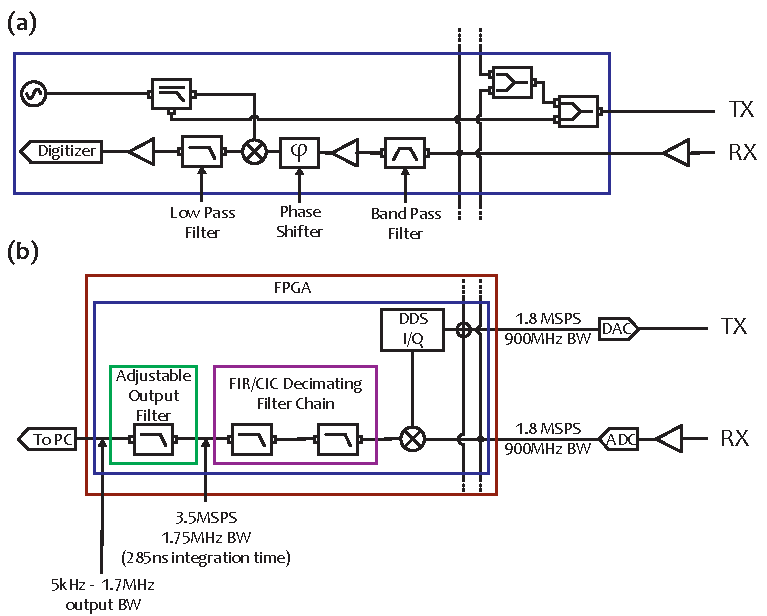
\includegraphics[width=0.8\linewidth]{Readout}
  \caption[Comparison of analog and digital multichannel readout]
  {\label{fig:multiread}(a) Schematic of an analog homodyne multichannel readout setup. Elements contained within the blue block must be repeated for each channel.
  A high-isolation band-pass filter is required per channel due to large non-linearities in the mixer. The use of a heterodyne receiver (not shown) allows phase
  sensitive detection, however requires a second analog signal generator. (b) The equivalent digital multichannel readout setup. Again, repeated elements are contained
  in the blue box, however in this case, all repeated elements are digital, hence require no additional hardware. Bandwidths for components used in our lab are shown.}
\end{figure}

Finally, we briefly touch on the topic of readout hardware at room temperature. The use of multiple simultaneous frequences for readout creates several challenges
for a typical analog homodyne detection architecture, due to the higher-order non-linearity and the inherent unscalability of analog signal generators and low-bandwidth
digitizers. A schematic of a typical analog readout chain is shown in Fig.~\ref{fig:multiread} (a). Due to the non-linearities present in the analog mixer, signals must be
band-pass filtered and boosted prior to mixing to achieve optimal signal-to-noise. For the homodyne setup shown, an analog phase shifter is required, and does not allow
phase information to be extracted. A second analog signal source may be added prior to the mixer to allow for heterodyne (I/Q) demodulation, however this significantly
increases the resource requirements of the circuit. Therefore even with frequency multiplexing near the device, the scalability of an analog readout setup is still
linear in the number of qubits. An equivalent digital circuit is shown in Fig.~\ref{fig:multiread} (b). For such a readout chain, all repeated elements are in digital logic,
hence, up to the resource limits of the FPGA, no additional hardware is required to increase the channel count. Above around 32 channels, an alternative approach becomes
necessary, which I flag in Sec.~\ref{sec:gooseberry}, however I will not present results here.

Having introduced the general structure of an architecture for a semiconductor based quantum computer, the remainder of this chapter deals with the practical implementation
of some architectures, which progressively reduce the power dissipated and resource requirements at each stage of the architecture, at the expense of flexibility.
Section~\ref{sec:primelines} proposes an architecture for a quantum computer that reduces the need for high-bandwidth wiring to low temperature, covers the distribution of pulses
at the qubit interface and introduces low power cryogenic switches to accomplish that goal. Section~\ref{sec:gooseberry} proposes an architecture that utilizes CryoCMOS to drastically
reduce the wiring requirements for a large scale quantum computer, and creates a platform for scaleable control of large numbers of qubits.

\clearpage
\section{Cryogenic Control Architecture for Large-Scale Quantum Computing}
\label{sec:primelines}
\import{chap2/}{arch}

\clearpage
\section{Gooseberry}
\label{sec:gooseberry}
%\import{chap2/}{arch}

\appendix
\chapter{Nanofabrication}
\label{sec:fab}
In this appendix, I will briefly outline the steps followed to fabricate the devices presented in this thesis.
Although there are several types of devices presented, including quantum dots, nanowire devices and Hall bars,
in each case the techniques used for each chip are adapted from the steps laid out below. The significant differences
in cleanroom tooling and safety protocols in each cleanroom mean that several procedures will likely need to
be adapted in order to gain similar results, however where possible I've tried to include all the details
that would be necessary to tailor the process to your own cleanroom.

\section{Fabrication Overviews}
\label{sec:fab_overview}

\subsection{Quantum Dot Nanofabrication}
\begin{enumerate}
    \item \textbf{Cleave Chips} (Sec.~\ref{sec:cleave})
    \item \textbf{Gallium Removal}: Remove gallium on the backside of wafer. (Sec.~\ref{sec:garem})
    \item \textbf{Chip Clean and Bake}: Remove any organic solvents and adsorbed moisture. (Sec.~\ref{sec:clean})
    \item \textbf{Alignment Mark Deposition}: Deposit TiAu alignment marks which will be our reference for all future fab steps. (Sec.~\ref{sec:metaldep})
    \item \textbf{Mesa Etch}: Define the active region of the device by etching away the 2DEG using a dilute \ce{H3PO4} solution. (Sec.~\ref{sec:mesaetch})
    \item \textbf{Ohmics Deposition}: Deposit AuGe ohmics and anneal into wafer. This step should be performed as soon as possible after the etch, preferrably on the same day. (Sec.~\ref{sec:ohmics})
    \item \textbf{Ohmic Contact Deposition}: Deposit bondpads for ohmic contacts. (Sec.~\ref{sec:metaldep})
    \item \textbf{Global Oxide Deposition}: Deposit a global \ce{Al2O3} or \ce{HfO2} oxide using ALD as a insulating barrier. (Sec.~\ref{sec:ald})
    \item \textbf{Gate Deposition}: Deposit surface gate pattern. (Sec.~\ref{sec:metaldep})
    \item \textbf{Gate Contact Deposition}: Deposit bondpads for surface gates. (Sec.~\ref{sec:metaldep})
\end{enumerate}

\subsection{InAs Hall Bar Nanofabrication}
\begin{enumerate}
    \item \textbf{Cleave Chips} (Sec.~\ref{sec:cleave})
    \item \textbf{Chip Clean and Bake}: Remove any organic solvents and adsorbed moisture. (Sec.~\ref{sec:clean})
    \item \textbf{Mesa Etch}: Define the active region of the device by etching away the 2DEG. Note that if Al is grown on the surface, this must be removed (Sec.~\ref{sec:transene}) prior to the mesa etch. (Sec.~\ref{sec:mesaetch})
    \item \textbf{Al Removal}: Etch away excess Al from the surface of the hall bar. (Sec.~\ref{sec:transene})
    \item \textbf{Global Oxide Deposition}: Deposit a global \ce{Al2O3} or \ce{HfO2} oxide using ALD as a insulating barrier. (Sec.~\ref{sec:ald})
    \item \textbf{Gate Deposition}: Deposit surface gate pattern. (Sec.~\ref{sec:metaldep})
\end{enumerate}

\subsection{GaAs Hall Bar and Circulator Nanofabrication}
\begin{enumerate}
    \item \textbf{Cleave Chips} (Sec.~\ref{sec:cleave})
    \item \textbf{Gallium Removal}: Remove gallium on the backside of wafer. (Sec.~\ref{sec:garem})
    \item \textbf{Chip Clean and Bake}: Remove any organic solvents and adsorbed moisture. (Sec.~\ref{sec:clean})
    \item \textbf{Mesa Etch}: Define the active region of the device by etching away the 2DEG using a dilute \ce{H3PO4} solution. (Sec.~\ref{sec:mesaetch})
    \item \textbf{Ohmics Deposition}: Deposit AuGe ohmics and anneal into wafer. This step should be performed as soon as possible after the etch, preferrably on the same day. (Sec.~\ref{sec:ohmics})
    \item \textbf{Gate Contact Deposition}: Deposit bondpads for surface gates. (Sec.~\ref{sec:metaldep})
\end{enumerate}

\section{Detailed Process Recipes}
\subsection{Cleave Chips}
\label{sec:cleave}
In the following section I will only describe the process for manual cleaving of chips using a diamond tip pen.
For more precise jobs, the use of a scribing tool which is able to better align and scribe chips is recommended.
For most III-V materials (100 orientation), you will only be able to scribe parallel to or perpendicular to the wafer flat.
Note that all steps should be performed on a cleanroom wipe which is to be disposed in a contaminated (III-V) waste bin
once the process is complete, due to the hazardous nature of III-V materials.
\begin{enumerate}
    \item Find wafer in fabrication logbook. Note previously scribed pieces and orientation. Select a piece to scribe. Record selected chip orientation and position in fabrication logbook.
    \item Line up the chip with the edge of a metal ruler. Using a diamond pen, make a small scratch (< \SI{1}{\milli\meter}) to the wafer edge.
    \item Balance the chip on the edge of a glass side with the scratch aligned to the edge of the slide.
    \item Press the overhanging section of the chip with filter paper or a cleanroom wipe to cleave the chip. The cleave should be clean and along the scratch direction.
    \item Choose a corner of the chip as a reference for future steps. Make a drawing of the scratches/features of the chip relative to the corner in the fabrication of logbook. Note the wafer orientation relative to the chip for future reference.
    \item Put contaminated filter paper/wipes in the contaminated wase bin, and glass slides into the sharps disposal.
\end{enumerate}

\subsection{Gallium Removal}
\label{sec:garem}
Ga metal is used as a sticking layer and thermal contact in the MBE chamber during heterostructure growth. When wafers
arrive from growers they often have this sticking layer still on their backsides, which must be removed prior to further processing
as it has a melting point of \SI{29}{\celsius} and has a tendency to contaminate process equipment and coat the surface of glassware.
We use the low melting point of Ga to physically remove it using q-tips followed by an optional \ce{HCl} dip to etch away any remnants.
The \ce{HCl} dip is useful to obtain the lowest possible ohmic resistances and is used more for Hall chips than quantum dots.
\begin{enumerate}
    \item Heat a small amount of NMP to \SI{80}{\celsius} in the designated NMP-(Gallium) beaker. It should be sufficiently full to cover the chip that will be placed in step 3. Prepare a small amount of NMP in an NMP-(Clean) beaker.
    \item Deposit 1-2 drops of PMMA onto the bottom third of a clean glass slide.
    \item Carefully place the GaAs chip facedown on the PMMA droplet, attempting to keep the back dry and free of resist.
    \item Place the glass slide on a \SI{95}{\celsius} hotplate for at least \SI{1}{\minute}.
    \item Using a cleanroom q-tip, gently wipe the Ga from the back of the chip, replacing the q-tip as necessary. Ensure that the chip does not move during this process as movement may damage the chip surface. The chip may be placed on the hotplate for an extra \SIrange{20}{30}{\second} if the Ga has dried.
    \item Place the glass slide in the heated NMP-(Gallium) beaker such that it is covered. Gently nudge the chip after \SI{30}{\second} until it is free of the slide and discard. Transfer the chip into the second NMP-(Clean) beaker.
    \item \textbf{Optional:} If at this point the gallium is sufficiently removed we may proceed directly to the chip clean and bake (Sec.~\ref{sec:clean}). Otherise transfer the chip to an IPA-(Clean) beaker with a small amount of IPA and sonicate for \SI{1}{\minute}.
    \item Spin and bake AZ6612, PMMA or a similar photoresist (Sec.~\ref{sec:spin}). In general ZEP or CZAR should be avoided for acid etches.
    \item Stir the chip in a \SI{37}{\percent} \ce{HCl} solution for \SIrange{2}{3}{\minute}.
    \item Rinse the chip in distilled \ce{H2O} for \SI{30}{\second}.
    \item Proceed to chip clean and bake (Sec.~\ref{sec:clean})
\end{enumerate}

\subsection{Clean and Bake}
\label{sec:clean}
The clean and bake step is used to remove any surface contaminants that may have been introduced in shipping and handling, as well as to
remove any surface moisture. Each solvent step should include some sonication during the \SI{5}{\minute} soak. Sonication may be performed for
the full \SI{5}{\minute} if desired. Tweezers should be washed in between each transfer step to prevent cross contamination.

\note{Al is easily damaged by NMP if the solvent has absorbed any moisture from the air. For materials with thin-film epitaxially grown Al, an alternative
solvent such as 1,3-Dioxolane should be used.}

\begin{enumerate}
    \item Place chip, face up, in a small amount of NMP at \SI{80}{\celsius} in an NMP-(Clean) beaker for at least \SI{5}{\minute}, with sonication.
    \item Transfer the chip to acetone in an Acetone-(Clean) beaker for at least \SI{5}{\minute}, with sonication.
    \item Transfer the chip to IPA in an IPA-(Clean) beaker for at least \SI{5}{\minute}, with sonication.
    \item Remove the chip from the IPA and dry with nitrogen on a fresh cleanroom wipe.
    \item Bake the chip at \SI{200}{\celsius} for \SI{5}{\minute}.
\end{enumerate}

\subsection{Resist Strip}
\label{sec:strip}
This process is used to strip resist of the surface of a chip, either due to a failed processing step or after a mesa etch (Sec.~\ref{sec:mesaetch}).
In the case that the strip is being performed during spinning, before the resist has been baked, it is usually sufficient to perform a quick \SI{30}{\second}
Acetone/NMP dip rather than the longer times prescribed below, as the resist will not be hardened. Sonication may be used to assist with the strip
as long as fine gates have not been evaporated. Otherwise sonication often damages these gates.

\note{ZEP, CZAR and other styrene based resists are \emph{NOT} compatible with Acetone. For these samples, NMP or an alternative solvent must be used.}

\note{Al is easily damaged by NMP if the solvent has absorbed any moisture from the air. For materials with thin-film epitaxially grown Al, an alternative
solvent such as 1,3-Dioxolane should be used.}

\begin{enumerate}
    \item Place chip, face up, in a small amount of NMP at \SI{80}{\celsius} in an NMP-(Clean) beaker, or Acetone in an Acetone-(Clean) beaker for at least \SI{3}{\minute}.
    \item Transfer the chip to IPA in an IPA-(Clean) beaker for at least \SI{30}{\second}.
    \item Remove the chip from the IPA and dry with nitrogen on a fresh cleanroom wipe.
\end{enumerate}

\newcommand{\spinunits}{(\si{\rpm})-(\si{\second})-(\si{\rpm\per\second})}
\subsection{Resist Spin}
\label{sec:spin}

\begin{table}
    \centering
    \hspace*{-1cm}
    \begin{tabular}{lllll}
        \toprule
        Process                                  & PMMA A3     & ZEP520A       & AZ6612       & LOR 5B\\
        \midrule
        Step 1 \spinunits                        & 500-5-1000   & 500-5-1000   & 500-5-1000   & 500-5-1000   \\
        Step 2 \spinunits                        & 9000-5-4000  & 9000-5-4000  & 10000-20-4000& 10000-4-4000 \\
        Step 3 \spinunits                        & 4000-45-4000 & 4000-120-4000& 4000-20-4000 & 4000-60-4000 \\
        Bake (\si{\celsius})-(\si{\second})      & 180-60       & 180-120      & 95-60        & 170-300      \\
        Approx. Thickness (\si{\nano\meter})     & 80           & 220          & 800 - 1000   & 600 - 800    \\
        \bottomrule
    \end{tabular}
    \hspace*{-1cm}
    \caption[Spin recipes for various resists]
    {Spin recipes for various resists. Each step gives a spin speed, a spin time, and an acceleration, separated by dashes.
    Thicknesses quoted are approximate and will vary depending on chip size and resist age and temperature.}
    \label{tab:spin}
\end{table}

\begin{figure}
    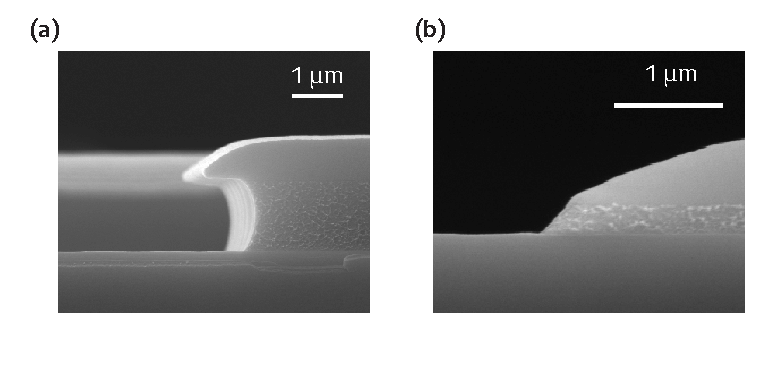
\includegraphics[width=0.85\linewidth]{resistedge}
    \caption[Edge profiles of two resists]
    {\label{fig:resistedge}Edge profiles of LOR 20B/AZ6612 (a) or LOR 5A/AZ6612 (b). The left image shows a significant undercut,
    suitable for deposition of thick metal layers, while the right image shows a smooth edge profile suitable for etching, and caused
    by the low solubility of LOR 5A relative to exposed AZ6612 in MIF300 developer. }
\end{figure}

The aim of spinning resist is to create a uniform thin film of a photoresist or electron-beam resist. Depending on the sort of process we wish
to run, with the developed resist, we may have different requirements for the edge profile. For evaporation of a metal stack with a liftoff process
we aim to create an undercut such that there is a break in the metal, with a height larger than the metal thichness we wish to evaporate. This can
be achieved using a thick single resist, which will in general have an undercut profile due to scattering of electrons or light through the resist, or by
the use of a bilayer resist stack, with a soluble polymer such as LOR-B or MMA as the underlayer. An example of a suitable undercut is shown in Fig.~\ref{fig:resistedge} (a).

For an acid etch, we would in general prefer a smooth edge profile with no undercut to ensure continuous flow of fresh acid over the
surface of the wafer and to ensure that acid is easily rinsed away once the etch is complete. In general this is achieved by a post-development
bake which will reflow resist at the edges of the developed region, and re-adhere resist to the surface of the wafer. An example of a
smooth edge profile is shown in Fig.~\ref{fig:resistedge} (b).

Spin parameters for various resists is given in Table~\ref{tab:spin}, which are valid only for small ($2.5 \times 5$ \si{\milli\meter} or $5 \times 5$ \si{\milli\meter})
samples. A very fast spin is used at the beginning of the spin to minimize the effect of the edge bead, which is a thick region of
resist around the edges of sample caused by surface tension. However, this spin is unsuitable for large samples or wafers and will lead
to variable resist thickness across the wafer, or, in the worst case, the wafer being flung from the chuck.

Hint: Squeezing the sides of the rubber puck makes it easier to move chips around. If the chip is not moving after the spin, try squeezing the
puck in a few locations and try again.

\note{If a resist was refrigerated, it must be allowed to warm to room temperature before use. Apart from the viscocity changing with temperature,
leading to an unpredictable resist thickness, the cold resist will condense moisture from the air, contaminating the resist for future users.}

\begin{enumerate}
    \item Clean the small rubber puck for chips with acetone on a cleanroom wipe.
    \item Attach your chip to the small rubber puck. Attempt to center it as much as possible.
    \item Take a few drops of resist with a pipette from the small resist bottle, making sure to not take from the bottom of the bottle.
    \item Dispense 2/3 dops of resist on the surface of the chip and begin the spin as soon as possible.
    \item After the spinning is complete, inspect the chip for a uniform spin. If the spin is not uniform or has picked up particulates, clean the resist (Sec.~\ref{sec:strip}).
    \item Bake the chip for the appropriate time.
    \item Clean the small rubber puck before finishing. Dispose of the pipette, do not replace unused resist.
\end{enumerate}

\subsection{Resist Develop}
\label{sec:develop}
Developing resist is the process of dissolving exposed (or unexposed for a negative tone resist) regions of resist to create a mask
on the surface of your sample. Depending on the chemistry of the process the solvent and times will vary. For the resist we've used,
development times are summarized in Table~\ref{tab:develop}.
\begin{table}
    \centering
    \hspace*{-1cm}
    \begin{tabular}{llll}
        \toprule
        Process                   & PMMA A3      & ZEP520A      & AZ6612 \\
        \midrule
        Solvent                   & MIBK:IPA 1:3 & o-Xylene     & MIF-300 (TMAH)\\
        Develop Time (\si{second})& 40           & 50           & 50            \\
        Rinse                     & IPA          & MIBK:IPA 1:3 & \ce{H2O}      \\
        Rinse Time (\si{second})  & 20           & 10           & 30            \\
        Second Rinse              & -            & IPA          & -             \\
        Rinse Time (\si{second})  & -            & 10           & -             \\
        \bottomrule
    \end{tabular}
    \hspace*{-1cm}
    \caption[Development recipes for various resists]
    {Development Recipes for various resists.}
    \label{tab:develop}
\end{table}

\note{Plasma ashing samples after the deposition of fine gates has been known to cause static damage.}

\begin{enumerate}
    \item Prepare beakers for each of the solvents necessary for that resist. There should be a dedicated, labelled beaker for each one.
    \item Place chip into each solvent for the requisite time, swirling the chip continuously. Try to move the chip between beakers quickly but smoothly at each step.
    \item Dry the sample with the \ce{N2} blow gun for $\approx \SI{30}{\second}$.
    \item If possible, plasma ash the sample for between \SIrange{5}{25}{\minute} for a photoresist, or \SIrange{20}{60}{\second} for a e-beam resist, immediately prior to the next step.
\end{enumerate}

\subsection{Mesa Etch}
\label{sec:mesaetch}
It is often necessary to define the sections where the 2DEG exists. For Hall measurements this is used to define the shape of the Hall bar.
For quantum dots, this is used to isolate devices from each other when multiple devices exist on a single chip, and to reduce parasitic
capacitance along readout or pulsing gates. In addition, it is possible to reduce crosstalk between gates by removing the 2DEG below
as much of the length of the gate as possible\cite{doi:10.1063/1.4752863}.

\begin{figure}
    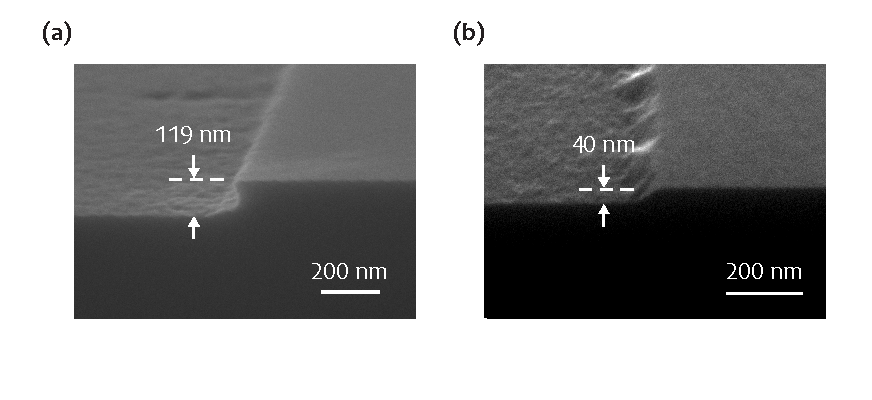
\includegraphics[width=0.85\linewidth]{EtchEdge}
    \caption[Etch profile of \ce{H2SO4} and \ce{H3PO4}]
    {\label{fig:etchedge}A comparison of the etch profiles of \ce{H2SO4} in (a) and \ce{H3PO4} (b). While \ce{H2SO4} leads
    to an anisotropic etch and a significant undercut, the \ce{H3PO4} leads to an isotropic etch and a smooth sidewall.}
\end{figure}

The use of a weaker phosphoric acid solution was chosen after a number of years of using a sulphuric acid solution as it was found that the
strength of the suphuric acid was leading to an anisotropic etch with a significant undercut. This had in past devices led to issues making
continuous gates over the edge of the mesa. The use of phosphoric acid in comparison leads to
an isotropic edge with a smoothly sloping sidewall, making the formation of continuous gates over the mesa edge easier.
A comparison of the etch profiles of \ce{H2SO4} and \ce{H3PO4} is given in Fig.~\ref{fig:etchedge}.

\begin{table}
    \centering
    \begin{tabular}{ll}
        \toprule
        Material & Etch Rate (\si{\angstrom\per\second}) \\
        \midrule
        Intrinsic GaAs & 12.1 \\
        GaAs Heterostructure & 15.9 \\
        InAs Heterostructure & 18.7 \\
        \bottomrule
    \end{tabular}
    \caption[Dilute phosphoric acid (5:1:50 \ce{H3PO4}:\ce{H2O2}:\ce{H2O}) etch rates]
    {Dilute phosphoric acid (5:1:50 \ce{H3PO4}:\ce{H2O2}:\ce{H2O}) etch rates}
    \label{tab:etchratess}
\end{table}

An additional bake is included in the processing after development to remove any undercut that may have developed in the resist during development.
In addition, the drying of the developer has been known to cause the resist to lift from the surface of the wafer near features, which is repaired
by this bake step. The addition of this step creates both smoother etch edges and better controlled edge thicknesses.

\begin{enumerate}
    \item Spin and bake AZ6612, PMMA or a similar resist (Sec.~\ref{sec:spin}). In general ZEP or CZAR should be avoided for acid etches.
    \item Expose the mesa pattern using the optical mask aligner or electron-beam lithography. Develop using the appropriate recipe (Sec.~\ref{sec:develop}).
    \item Postbake the resist using the same bake as the initial bake (see Table~\ref{tab:spin}) to remove any undercut and readhere the resist to the surface of the chip.
    \item Prepare a solution dilute phosphoric acid solution of \ce{H3PO4}:\ce{H2O2}:\ce{H2O} in a 5:1:50 ratio. Remember that acids should always be added to water, not the other way around. Stir thoroughly with PTFE (acid) tweezers, and leave to thermalize for $\approx \SI{30}{\minute}$.
    \item Measure the resist height with a surface profilometer (dektak in our case). Record in several locations.
    \item Pour some of the dilute phosphoric acid solution into a small etch beaker. Etch the chip for the appropriate time (use Table~\ref{tab:etchratess} for standard etch rates) using teflon tweezers and stirring continuously. I usually aim $\approx \SI{10}{\nano\meter}$ below the depth of the 2DEG. Etching too deeply can make it challenging to run gates to the surface of the 2DEG.
    \item Rinse in distilled \ce{H2O} for a minimum of \SI{30}{\second} and dry with nitrogen on a clean wipe.
    \item Measure the new height of the resist using a surface profilometer in the same locations as before. The etch depth is the difference between the two measurements. If the depth is insufficient, repeat steps 5-7.
    \item Strip resist (Sec.~\ref{sec:strip}).
\end{enumerate}

\subsection{Al Etch}
\label{sec:transene}
For InAs devices, aluminium must be selectively etched away to define device grometries. This is accomplished
using a Transene-D based wet etch. This process has been found to be highly sensitive to both temperature
and etch time, and hence care must be taken when performing this step if you wish to achieve reproducible
results. For this reason, a PID controller, glass thermometer and stirrer is necessary for high quality etches.

For a thin (\SI{8}{\nano\meter}) layer of epitaxially grown Al, we have had success using a \SI{11}{\second} etch
followed by two \SI{11}{\second} \ce{H2O} rinses, however this process must be optimized for local conditions.

\note{Transene-D will begin to degrade at temperatures above $\approx \SI{50}{\celsius}$. Care must be taken while heating to ensure this temperature is not exceeded, including at the base of the beaker. As such heating must be quite slow.}

\note{Tranene-D will oxidize if stirred too vigorously. The stirrer should be set to the lowest possible speed and should not visibly agitate the surface of the etch solution.}

\begin{enumerate}
    \item Spin and bake AZ6612, PMMA or a similar resist (Sec.~\ref{sec:spin}). In general ZEP or CZAR should be avoided for acid etches.
    \item Expose the mesa pattern using the optical mask aligner\ or electron-beam lithography. Develop using the appropriate recipe (Sec.~\ref{sec:develop}).
    \item Postbake the resist using the same bake as the initial bake (see Table~\ref{tab:spin}) to remove any undercut and readhere the resist to the surface of the chip.
    \item Prepare a solution of Transene-D, heated to \SI{47.5}{\celsius} with a PID controller, and stirred at low speed. Ensure this temperature is stable before beginning the etch.
    \item Prepare two beakers of DI-water for the rinse. Prepare a beaker of Acetone to strip the resist as soon as the etch is complete.
    \item Immediately prior to commencing the etch, stop the stirrer.
    \item Dip the sample in Transene using PTFE tweezers, agitating continously. Once complete, immeditately transfer to first water beaker, again agitating continuously, followed by the second water beaker.
    \item Transfer the chip as soon as possible to Acetone to strip the resist. Restart the stirrer.
    \item Follow the steps for stripping resist to finish (Sec.~\ref{sec:strip}).
\end{enumerate}

\subsection{Metal Deposition}
\label{sec:metaldep}
Deposition of metals is a repeated step for several of the processes. For all of the work presented in this thesis
we use a liftoff based process, however I will note that for sputtered metals or for ultra high-Q resonators such
a process may be unsuitable.

For thin gates, it is necessary to evaporate metals at a reasonably high rate, as slower deposition rates lead to larger
grain sizes which can cause discontinuities to appear in small gates. Although in general a faster deposition is preferable,
there are limits to how fast various metals will evaporate with a stable rate. Some recommendations are given in the Table~\ref{tab:evap}, however
these should be based tools (and the experiences of others using it) and tuned accordingly.

Metal compatibility should also be considered when choosing the tool to use for various evaporations. For tools handling CMOS processes
for example, the use of gold is unsuitable. For evaporators focussed on ultra high-Q resonators, nickel and other magnetic materials
will decrease transition temperature, but this may not be a limiting factor for your process.

Metal thicknesses for a number of processes are given in Table~\ref{tab:evap}.

\begin{table}
    \centering
    \begin{tabular}{llrr}
        \multicolumn{4}{c}{\textbf{Ohmics}}\\
        \toprule
        Step & Metal & Thickness (\si{\angstrom}) & Deposition Rate (\si{\angstrom\per\second}) \\
        \midrule
        Layer 1 & Ni & 50          & 2 \\
        Layer 2 & Ge & $x$  (350)  & 5 \\
        Layer 3 & Au & $2x$ (700)  & 5 \\
        Layer 4 & Ni & 180         & 2 \\
        Layer 5 & Au & 500  & 5 \\
        \bottomrule \\

        \multicolumn{4}{c}{\textbf{Fine Surface Gates}}\\
        \toprule
        Step & Metal & Thickness (\si{\angstrom}) & Deposition Rate (\si{\angstrom\per\second}) \\
        \midrule
        Layer 1 & Ti & 80  & 2 \\
        Layer 2 & Au & 120 & 5 \\
        \bottomrule \\

        \multicolumn{4}{c}{\textbf{Contact Gates and Alignment}}\\
        \toprule
        Step & Metal & Thickness (\si{\angstrom}) & Deposition Rate (\si{\angstrom\per\second}) \\
        \midrule
        Layer 1 & Ti & 120         & 2 \\
        Layer 2 & Au & 1000 - 2000 & 5 \\
        \bottomrule
    \end{tabular}
    \caption[Evaporator recipes]
    {Evaporator recipes for various processes. Note that for ohmics, the depth of the middle two layers should be varied
    depending on the depth of the 2DEG, such that $3x \approx d$. Values used successfully for a \SI{91}{\nano\meter} are given
    in brackets.
    }
    \label{tab:evap}
\end{table}

\note{ZEP, CZAR and other styrene based resists are \emph{NOT} compatible with Acetone. For these samples, NMP or an alternative solvent must be used.}

\note{After fine gates are deposited, use of sonication can cause damage to gates. Limit sonication to about \SI{15}{\second} at low power and use only if necessary.}

\note{Drying your sample before liftoff is complete will cause unwanted sections of metal to adhere to the surface of your chip, making them very difficult (if not impossible) to remove.}

\begin{enumerate}
    \item Spin and bake photoresist or e-beam resists (Sec.~\ref{sec:spin}).
    \item Expose the pattern using the optical mask aligner or electron-beam lithography. Develop using the appropriate recipe (Sec.~\ref{sec:develop}).
    \item Mount samples in evaporator. You can optionally mount samples to a glass slide if features exist close to edges along all 4 sides of the chip. In this case, use a drop of PMMA A3 on a glass slide, place the chip on the drop and bake for \SI{60}{\second} at \SI{90}{\celsius} or until resist is dried. Avoid higher temperatures for risk of reflowing resist and melting the undercut.
    \item Pump evaporator until sufficiently low pressure and evaporate according to the given procedure for your evaporator.
    \item Allow chip to cool for $\approx \SI{5}{\minute}$ before venting. Remove samples.
    \item Place a small amount of NMP into the NMP-(Liftoff) beaker and heat to \SI{80}{\celsius}. Leave for \SIrange{30}{60}{\minute}.
    \item Sonicate for $\approx \SI{30}{\second}$ to clear remaining metal of the surface. Visually inspect while wet leaving for additional time if liftoff is not complete.
    \item A spray with Acetone or IPA from a squeeze bottle may assist you in removing stubborn sections of metal.
    \item After liftoff is complete, place the chip in the IPA-(Liftoff) beaker for \SI{3}{\minute}.
    \item Remove chip and dry with \ce{N2} blowgun on a cleanroom wipe.
\end{enumerate}

\subsection{Ohmics Deposition}
\label{sec:ohmics}
Ohmic contacts are used to make contact to the 2DEG from the surface of the chip and are formed using a eutectic stack
of AuGe. Nickel is used as a sticking layer to the surface of the GaAs and a diffusion barrier which allows only Ge to diffuse
into the semiconductor, followed by a Au:Ge in a 2:1 ratio, which forms our eutectic alloy. This is capped by a further Ni and
Au layer to prevent oxidation. The exact stack for a 91nm 2DEG is given in Table~\ref{tab:evap}. For use with shallower or
deeper 2DEGs, the thickness of the centeral Ge and Au layers must be modified. The contact to the 2DEG is made by a degenerately
Ge doped section of semiconductor that is formed under the metal stack~\cite{RELLING1989380,PIOTROWSKA1983179}.

\begin{figure}
    \includegraphics[width=0.8\linewidth]{Ohmic}
    \caption[Sample ohmic design and anneal]
    {\label{fig:ohmic}(a) Sample ohmic design, showing the mesa in yellow and the ohmic metal stack in green. The mesa contains slices
    to increase the ohmic contact with the edge along multiple crystallographic orientations, and the ohmic metal extends past the edge.
    (b) Optical micrograph of a low resistance ohmic. Note the bubbly appearance of the surface. A ovoid mark is visible in the center of the
    pad where a bond was placed to test the contact. (c) SEM image of an annealed ohmic.}
\end{figure}

The design of ohmics is particularly important for quantum Hall samples, where making good contact to the edge along multiple
crystalographic orientations is crucial, particularly at high field. In addition, to obtain the lowest possible ohmic resistance,
we have found it necessary to make the ohmic stack extend over the edge of the mesa. This allows the ohmic to anneal in along the
side wall to improve the area of the contact. We use a design adapted from~\cite{2007PhDTM}. A sample of such an ohmic is given in Fig.~\ref{fig:ohmic}.

Annealing is performed in a rapid thermal annealer, in our case the MILA-5000, in an atmosphere of forming gas (4\% \ce{H2}:96\% \ce{N2}).
We have found it necessary to place samples on a SiC heat spreader, which contains an integrated thermocouple in order to accurately
measure the temperature of chips during the annealing process. For devices with a deeper 2DEG (i.e. 400nm for high mobility Hall samples)
it may be necessary to increase the anneal time to account for the increased depth.

Good ohmics will appear uniformly bubbly after annealing, with no dark spots. The surface of the sample should not change, and color change
may indicate contamination on the surface of the chip prior to annealing. I have found a round of plasma ashing immediately before the anneal
may be necessary to remove contamination.

\begin{table}
    \centering
    \begin{tabular}{lrr}
        \toprule
        Step & Temperature (\si{\celsius}) & Time (\si{\second}) \\
        \midrule
        Step 1 (Ramp) & 130 & 8 \\
        Step 2 (Hold) & 130 & 130 \\
        Step 3 (Ramp) & 450 & 20 \\
        Step 4 (Hold) & 450 & 90 \\
        \bottomrule
    \end{tabular}
    \caption[Rapid thermal anneal recipe]
    {Recipe for the ULVAC MILA-5000 rapid thermal annealer, using a forming gas (4\% \ce{H2}:96\% \ce{N2}) atmosphere. Note that the PID parameters must be appropriately tuned
    to ensure temperatures are reached rapidly without overshoot.}
    \label{tab:anneal}
\end{table}

\begin{enumerate}
    \item Evaporate and lift off ohmics pattern (Sec.~\ref{sec:metaldep}). Ensure the surface is clear of contaminants. If in doubt, the chip may be plasma ashed prior to loading into the annealer.
    \item Vent the annealer for \SI{3}{\minute} with nitrogen prior to loading sample. Following sample loading, purge the chamber with forming gas for \SI{3}{\minute} prior to beginning the process.
    \item Anneal chips in an atmosphere of forming gas (4\% \ce{H2}:96\% \ce{N2}), following instructions for the local tool. A sample set of parameters is given in Table~\ref{tab:anneal} which has been found to give low resistance ohmics in our lab.
    \item After the anneal is complete, immediately purge the chamber with nitrogen gas at high flow to assist with cooling. Allow the sample to cool to \SI{50}{\celsius} prior to unloading.
\end{enumerate}

\subsection{Oxide Deposition (ALD)}
\label{sec:ald}
ALD is deposited on samples as an insulating dielectric, either to minimize leakage to the donor layer which
is hypothesized to be a source of charge noise~\cite{PhysRevB.72.115331}, or as an insulating layer for
multi-layer devices. The addition of this step to spin qubit devices is a reasonably recent addition to our
fabrication process and over time this process has been optimized to increase the quality of the dielectric
that is grown. Initially we had been using a lift-off process~\cite{doi:10.1063/1.1612904}, however such a process
was found to grow measurably worse quality oxide films, due to the low temperature of growth required for resist
compatibility (\SIrange{90}{150}{\celsius}), and contamination due to resist in the process chamber.

Our current process therefore deposits a global oxide, grown at a minimum temperature of \SI{200}{\celsius}.
We make contact to lower layers either by bonding through the oxide, or using a selective Al etchant to remove
sections of the oxide. In general, the highest possible growth temperature will result in the highest oxide
quality, where materials compatibility is taken into account (In will precipitate out of InAs above \SI{250}{\celsius} for example).

For devices in this thesis, we've grown both \ce{Al2O3} and \ce{HfO2} oxides using TMA and TDMA-Hf as precursors and
\ce{H2O} as an oxidising agent. In general we've not had success with \ce{O3} as an oxidizer, with the quality of film
grown lowered relative to \ce{H2O}. Although there will be variance by tool and growth temperature, as a rule of thumb,
we've found 100 cycles of TMA at \SI{200}{\celsius} to grown approximately \SI{8}{\nano\meter} of oxide.

\note{Avoid placing samples with resist in the growth chamber as it leads to significantly decreased oxide quality.}

\begin{enumerate}
    \item Set the chamber temperature to the correct growth temperature for the growth. Allow the chamber temperature to settle prior to loading your sample.
    \item Set the correct number of cycles for your oxide growth. The thickness of oxide grown per cycle with vary depending on the tool and the temperature of the growth.
    \item Load your sample, and a blank silicon piece, into the growth chamber. For load locked tools, allow the stage to reach the correct temperature before beginning the process.
    \item Run the ALD growth program. It is usually worth checking that there are pressure spikes for the first few cycles to ensure precursors have not been depleted.
    \item Once the process is complete, unload the samples. Check the depth of deposited oxide using an ellipsometer on the blank Si chip and record this value.
\end{enumerate}
%% This defines the bibliography file (main.bib) and the bibliography style.
%% If you want to create a bibliography file by hand, change the contents of
%% this file to a `thebibliography' environment.  For more information
%% see section 4.3 of the LaTeX manual.
\begin{singlespace}
\renewcommand*{\doi}[1]{\href{https://doi.org/\detokenize{#1}}{doi: \textcolor{blue}{\detokenize{#1}}}}
\renewcommand*{\backrefalt}[4]{%
    \ifcase #1 %
        No citations.%
    \or
        Page: #2%
    \else
        Pages: #2%
    \fi
}
\bibliography{intro,main,chap1,chap2,chap3,chap4}
\bibliographystyle{unsrtnat_mod}
\end{singlespace}

\end{document}

